\begin{filecontents*}{example.eps}
%!PS-Adobe-3.0 EPSF-3.0
%%BoundingBox: 19 19 221 221
%%CreationDate: Mon Sep 29 1997
%%Creator: programmed by hand (JK)
%%EndComments
gsave
newpath
  20 20 moveto
  20 220 lineto
  220 220 lineto
  220 20 lineto
closepath
2 setlinewidth
gsave
  .4 setgray fill
grestore
stroke
grestore
\end{filecontents*}
\RequirePackage{fix-cm}
%\documentclass{svjour3}                    % onecolumn (standard format)
\documentclass[smallcondensed]{svjour3}     % onecolumn (ditto)
%\documentclass[smallextended]{svjour3}       % onecolumn (second format)
%\documentclass[twocolumn]{svjour3}          % twocolumn
%
\smartqed  % flush right qed marks, e.g. at end of proof
%
\usepackage{amsmath}
\DeclareMathOperator{\sech}{sech}
\usepackage{graphicx}
\usepackage{subfig}
\graphicspath{{../Fig/}}
\journalname{J. SCI. COMPUT.}


\begin{document}

\title{KdV Equation and Computations of Solitons: Nonlinear Error Dynamics}


\author{Ashwin V. M.\and K. Saurabh \and Sriramkrishnan M.\and  P. M. Bagade\and Parvathi M. K. \and Tapan K. Sengupta }

\institute{Tapan K. Sengupta \at
              High Performance Computing Laboratory \\
              Department of Aerospace Engineering \\
              I. I. T. Kanpur 208 016 \\
              INDIA\\
              Tel.: +91-512-2597945\\
%              Fax: +123-45-678910\\
              \email{tksen@iitk.ac.in}           %  \\
%             \emph{Present address:} of F. Author  %  if needed
%           \and
}

%\date{Received: date / Accepted: date}
% The correct dates will be entered by the editor


\maketitle

\begin{abstract}
Here we have developed new compact and hybrid schemes for the solution of KdV equation. These schemes for the third derivative have been analyzed 
in the spectral plane for their resolution and compared with another scheme in the literature. Furthermore the developed schemes have been used
to solve a model linear dispersion equation. The error dynamics equation has been developed for this model equation. Despite the linearity of the 
model equation, one can draw conclusions for error dynamics of nonlinear differential equations. The developed compact scheme has been found to be 
quite accurate in solving KdV equation. One- and two-soliton cases have been reported to demonstrate the above.

\keywords{KdV equation \and Solitons \and Nonlinear error dynamics \and  Compact scheme \and DRP scheme \and Gibbs' phenomenon}
 
\end{abstract}



\section{Introduction}

The Korteweg-de Vries equation or KdV equation, as is generally known, was proposed in \cite{Informa} to simulate the observations and experimental findings of Russell \cite{Russell1844} on a distinct class of surface gravity waves convecting as an equilibrium solution indicating a balance between dispersion effects and nonlinearity, both of which originate due to convection. The KdV equation admits certain solitary waves or ``solitons" for specific initial conditions as described later. The identity of a soliton was defined in \cite{Drazin1989} as ``any solution of a nonlinear equation or system which (i) represents a wave of permanent form; (ii) is localized; (iii) can interact strongly with other solitons and retain its identity." Provided a delicate balance between the steepening effect of nonlinearity and dispersion effect of attenuation of the wave-packet, as governed by the KdV equation is maintained, such waves can be realized computationally only with adequate care. As we will explain here that in the presence of error sources, Gibbs' phenomenon will be observed in the computed solution, even when the permanent form of the solitary wave is approximately maintained. While in the texts \cite{Drazin1989}
and published literature \cite{Fornberg1978} effects of error in prescribing initial condition is highlighted by comparing with the exact eigen solution obtained from an equivalent Sturm-Liouville problem, in the present study we include other sources of errors, as given by an error propagation equation developed from a model convection equation describing predominantly the effects of dispersion. 

This equation has over the past decades, through rigorous analytical studies, transcended the domain of hydrodynamics and, joined the ranks of the Nonlinear Schr\"odinger (NLS) equation and the Fermi-Pasta-Ulam (FPU) problem in the field of nonlinear dynamics \cite{Zabusky2005a}. Solitons and 
soliton-like solutions have been observed in the study of solid state physics \cite{Seeger1953} and optics \cite{Hasegawa1973}. Following the first numerical solution in \cite{Zabusky1965}, the KdV equation has attracted a revived interest in its computing. Infinitely many conservation laws related 
to certain properties of solution of KdV equation were reported in \cite{Miura1968,Whitham1965}. The most important contributions were reported in 
\cite{Gardner1967,Lax1968}, in the form of the inverse scattering transform (IST) method which paved the way for evaluating exact solutions of the KdV equation for specific initial states. Existence of exact solutions reveal the possibility of KdV equation as a model equation to test numerical methods designed for convection dominated nonlinear problems, such as the Navier-Stokes equation to estimate nonlinear error dynamics. 

Many novel numerical methods were formulated in the past to simulate the KdV equation. Two ``dissipative finite difference schemes" were constructed in \cite{Vliegenthart1971} which naturally do not follow the exact solution. The intention in developing such dissipative schemes was to eliminate high wavenumber components of the solution via attenuation by numerical diffusion, which otherwise lead to numerical instability. However, it would be shown 
here that even a diffused solution leads to Gibbs' oscillations from the foot of the soliton \cite{Sengupta2004a}.

A comprehensive comparison of different numerical schemes were made in \cite{Taha1984}. Among the numerical methods reviewed in \cite{Taha1984}, the notable ones were the explicit method due to Zabusky and Kruskal \cite{Zabusky1965}, a semi-implicit scheme based on IST and the pseudo-spectral method due to Fornberg and Whitham \cite{Fornberg1978}. The latter two were reported to be the most accurate representation of the KdV equation. However, the maximum error in very early stages of these simulations were of the order of $10^{-3}$ to $10^{-2}$. Some of the shortcomings 
could be attributed to the use of three-time level leapfrog method for time integration, which induces spurious computational modes, as shown in \cite{Sengupta2013a,Sengupta2004}. Additionally, the pseudo-spectral method is less accurate, and yet computationally intensive, as this requires three to 
four fast Fourier transforms at each time-step.

In \cite{Argyris1987}, Petrov-Galerkin method was applied to the KdV equation and reported the presence of error as a measure of computational imbalance between non-linearity and dispersion. Ascher and McLachlan \cite{Ascher2004} adopted semi-explicit multisymplectic box schemes in an attempt to improve on the dispersion relation preserving (DRP) properties.

Compact schemes for spatial discretization have better resolution and thus would yield a closer approximation in preserving the dispersion relation. First application of compact schemes on KdV equation was reported in \cite{Li2006} wherein, \emph{fourth} and \emph{sixth order} compact schemes for first and third derivatives were used. However, the simulated results were not insightful towards the practical efficacy of these schemes, as the work reported error levels at early time instants only.

This present work is an attempt to refine numerical simulation of the KdV equation by employing high accuracy compact schemes \cite{Sengupta2013a,Sengupta2006b}. As most of the high accuracy schemes are developed for first and second derivatives, here an optimized stencil for third derivative has been developed with the sole intention of solving the KdV equation indefinitely with DRP properties. A quantitative comparison of numerical properties of compact schemes against conventional finite difference schemes has been used here in explaining the results and identifying the sources of error in a systematic manner, following the earlier work in \cite{Sengupta2007}.

The document is organized in the following manner. Section \ref{sec:goveq} describes the governing equation, exact solutions for a given initial condition and how the initial condition affects the evolution of the numerical solution. Section \ref{sec:num_sch} elaborates on the numerical schemes used, wherein the design of two new methods to evaluate third derivative by implicit and hybrid methods are introduced. In section \ref{sec:err}, an analysis on error propagation in the simulation of the one-dimensional dispersion equation is reported, so as to identify the sources of error in a dispersive equation. Section \ref{sec:res} presents the time evolution of numerical solution and corresponding error for \emph{one-soliton} and \emph{two-soliton} cases for various schemes used. Finally, section \ref{sec:sum} briefly highlights the observations made in this exercise.
%-----------------------------------------------------------------------------------------------------
\section{Governing Equation and Exact Solutions}
\label{sec:goveq}
The original KdV equation as expressed in \cite{Informa} incorporates parameters such as height of the solitary wave, ratio of amplitude of the wave to the height of fluid underneath and so on. From an analytical point of view, the following standard non-dimensional form of the KdV equation has been used in the literature \cite{Taha1984}.

\begin{equation}
\label{eq:kdv}
u_t + 6 uu_x + u_{xxx} = 0
\end{equation}

The above equation can be reformulated in the conservation form before discretizing. Two such forms have been used here, as follows

\begin{equation}
\label{eq:ckdv1}
\frac{\partial}{\partial t}u + \frac{\partial}{\partial x} \left(3 u^2 + u_{xx}\right) = 0
\end{equation}

\begin{equation}
\label{eq:ckdv2}
\frac{\partial}{\partial t}u +  \frac{\partial}{\partial x}(3u^2) + \frac{\partial^3}{\partial x^3}u = 0
\end{equation}
These equations are solved numerically in a periodic domain to avoid difficulties arising out of reflections from the non-periodic boundaries. The finite difference schemes developed here are central in nature. Applying periodic boundary conditions, present methods can be computed for an indefinite time, while not being influenced by the use of one-sided space discretizations for boundary closure. By doing so, one could clearly demonstrate which numerical method is less erroneous for tracking nonlinear dynamics.

\subsection{Initial Condition and Exact Solutions}
\label{subsec:init}
The KdV equation admits solitary wave solutions for initial conditions of the form, $u_0 = A_0 \sech^2x$. Many classes of exact solutions exist from 
one- to N-solitons solutions. The amplitude of the initial condition, $A_0$ determines how many solitons emerge as time evolves. Here, we shall focus 
on one- and two-solitons solutions only.

\subsubsection{One-soliton solution} In this case, a single soliton convects with a phase speed which is linearly proportional to the amplitude. The initial condition and exact solution, respectively, are given by
\begin{align}
\label{eq:1solin}
u(x,0) = &2 \sech^2 x\\
\label{eq:1solex}
u(x,t) = &2 \sech^2(x-4t)
\end{align}

\subsubsection{Two-soliton solution} The following initial condition has as interesting feature of non-linear interaction arising out of two-soliton solution
\begin{equation}
\label{eq:2solin}
u(x,0) = 6 \sech^2 x
\end{equation}
In this case, as the solution evolves, the initial profile breaks into two distinct solitons, one of it having amplitude eight and the other having an amplitude two. With these two components of solution located sufficiently apart, the exact solution is a superposition of the two given by  
\begin{equation}
\label{eq:2solex}
u(x,t) \approx  8 \sech^2 \left(2\xi - \frac{1}{2} ln 3\right) + 2 \sech^2 \left(\eta + \frac{1}{2} ln 3\right)
\end{equation}
where, $\xi =x-16t$ and $\eta=x-4t$. Once again, the phase speeds of the exact solution components are related to the amplitude of the solitons, with the higher amplitude soliton traveling four times faster than the lower amplitude soliton.

In a periodic domain, these two solitons will continuously keep interacting. When this event occurs, the taller soliton shows a phase lead of $ln 3$ and the shorter soliton shows a phase lag of $ln 3$, relative to their corresponding phases before interaction. There are many possible soliton components, depending upon the initial condition and this is discussed next.

\subsection{Reflectionless Potentials}
\label{subsec:ref}
Specifying a reflectionless potential as initial condition and maintaining its amplitude is crucial for accurate simulation of the KdV equation. The inability to achieve this computationally due to restrictions imposed by discretization is observed as a form of error. The source of such error is explained in this section.

In \cite{Miura1968}, it was shown that the transformation, $u = v^2 + v_x$ used in Eq. \eqref{eq:kdv} would yield an equation, known as \emph{modified KdV} or \emph{mKdV equation}, the solution of which would also be the solution of the original KdV equation. This transformation, known as \emph{Miura transformation}, when substituted with $v = {\psi_x}/{\psi}$ converts Eq. \eqref{eq:kdv} to $\psi_{xx}-u\psi=0$. Since, the KdV equation is Galilean invariant, it is possible to transform the variables from $ x \to x+\lambda t;\; u \to u - \lambda$, and thus, Miura transformation can be represented by means of the time-independent Sturm-Liouville equation \cite[pp. 64-66]{Drazin1989}.
\begin{equation}
\label{eq:sturm}
\psi_{xx} + (\lambda - u_0) \psi = 0
\end{equation}
Hence, the relation of the Sturm-Liouville equation to the KdV equation has been established. Solving Eq. \eqref{eq:sturm}, for a given initial profile or ``potential function", $u_0(x,0)$, constitute the scattering problem. In the limit, $|x| \to \infty$ with $u \to 0$ asymptotically, the modes or eigenfunctions of the Eq. \eqref{eq:sturm} can be generally represented as oscillatory functions of the form $\hat{\psi} \sim e^{\pm ikx}$, where the wavenumber is related by $k=\sqrt{\lambda}$. For $\lambda>0$, we would have a continuous spectrum of eigenvalues, with the corresponding eigenfunctions given by

\begin{equation*}
\label{eq:sturm_bc}
\hat{\psi} \approx
\begin{cases}
e^{ikx} + b(k)e^{-ikx} & \text{as } x \to -\infty,\\
a(k)e^{ikx} & \text{as } x \to +\infty
\end{cases}
\end{equation*}

\begin{figure}[h!]
\center
 \includegraphics[width=0.9\linewidth]{Fig_1}
  \caption{Schematic representing different wave components of the solution to Sturm-Liouville equation as given in \cite{Drazin1989}.}
  \label{fig:scatter}
\end{figure}

Any arbitrary error can be represented in terms of these eigenfunctions. Thus, the error associated with the numerical solution of the KdV equation 
can be characterized based on these eigenfunctions, which is illustrated in Fig. \ref{fig:scatter}. The error can be represented by Fourier-Laplace component in a general framework. If the unit of such error is represented by a component with unit amplitude identified as the \emph{incident} wave appearing from inlet of the computational domain (shown as originating from $-\infty$), then upon traversing through the scatterer, the incident wave decomposes into two, a \emph{transmitted} wave of amplitude $a(k)$ and a \emph{reflected} wave of amplitude $b(k)$. It has been shown in \cite{Drazin1989} that the reflected and transmitted component amplitudes follows the identity, $|a|^2 + |b|^2 =1$. In this reference, effect of imperfect initial condition has been investigated for the creation of error, noting that the reflected component dominates over the transmitted component. For a reflectionless scattering potential $u_0$, one requires $b(k)=0$, implying a clean transmission of the error with amplitude given by $a(k) = 1$.

The choice of general initial condition of the form, $u_0 = A_0 \sech^2{x}$ is known to have solitary wave solution only without any error for particular choices of $A_0$. In the presence of any error, the transmitted and reflected error components are obtained by solving the equivalent Sturm-Liouville problem \cite[pp. 42-48]{Drazin1989}, with the scattering coefficients obtained as
\begin{align*}
a(k) = \frac{ \Gamma(\tilde{a})\Gamma(\tilde{b}) }{ \Gamma(\tilde{c})\Gamma(\tilde{a}+ \tilde{b} -\tilde{c}) };  \; 
b(k) =\frac{  a(k) \Gamma(\tilde{c})\Gamma(\tilde{c}- \tilde{a} -\tilde{b}) } { \Gamma(\tilde{c} -\tilde{a})\Gamma(\tilde{c} - \tilde{b}) }
\end{align*}
where, $\tilde{a} = \frac{1}{2} - ik + \sqrt{A_0 + \frac{1}{4}}$, $\tilde{b} = \frac{1}{2} - ik - \sqrt{A_0 + \frac{1}{4}}$, and $\tilde{c} = 1 - ik$. If the amplitude of the initial condition is $A_0= N(N+1)$ where $N$ is any positive integer, we get $a(k)=1, b(k)=0$ for all $k$, i.e., there are no errors in the form of reflected and transmitted components.

It is also interesting to note that the poles of the eigenfunctions, i.e., the discrete eigenvalues for which $a(k)$ and $b(k)$ are undefined, determine the number of solitons obtained. There exists a property of the Gamma function, due to which it is undefined for zero and for negative integers. 
Therefore, we encounter these poles when $\tilde{b}=0,-1,-2...$, in the upper half of the complex $k$-plane. For a general $A_0$, the number of such discrete eigenvalues is restricted by the ceiling value of:
\begin{equation}
\label{eq:ao_n_relation}
\sqrt{A_0 + \frac{1}{4}} - \frac{1}{2} \equiv N
\end{equation}

Furthermore in \cite{Gardner1967}, by solving inverse scattering problem it is shown that given an initial condition, the corresponding exact solution 
can be evaluated analytically for reflectionless potentials. However for the case with $b(k)\neq 0$ the solution would contain a reflected component or 
a dispersive wave component observed as a ``tail" propagating upstream from the left shoulder of the soliton. Such Gibbs' phenomenon is demonstrated in Fig. \ref{fig:reflect}.

\begin{figure}[h!]
\centerline{
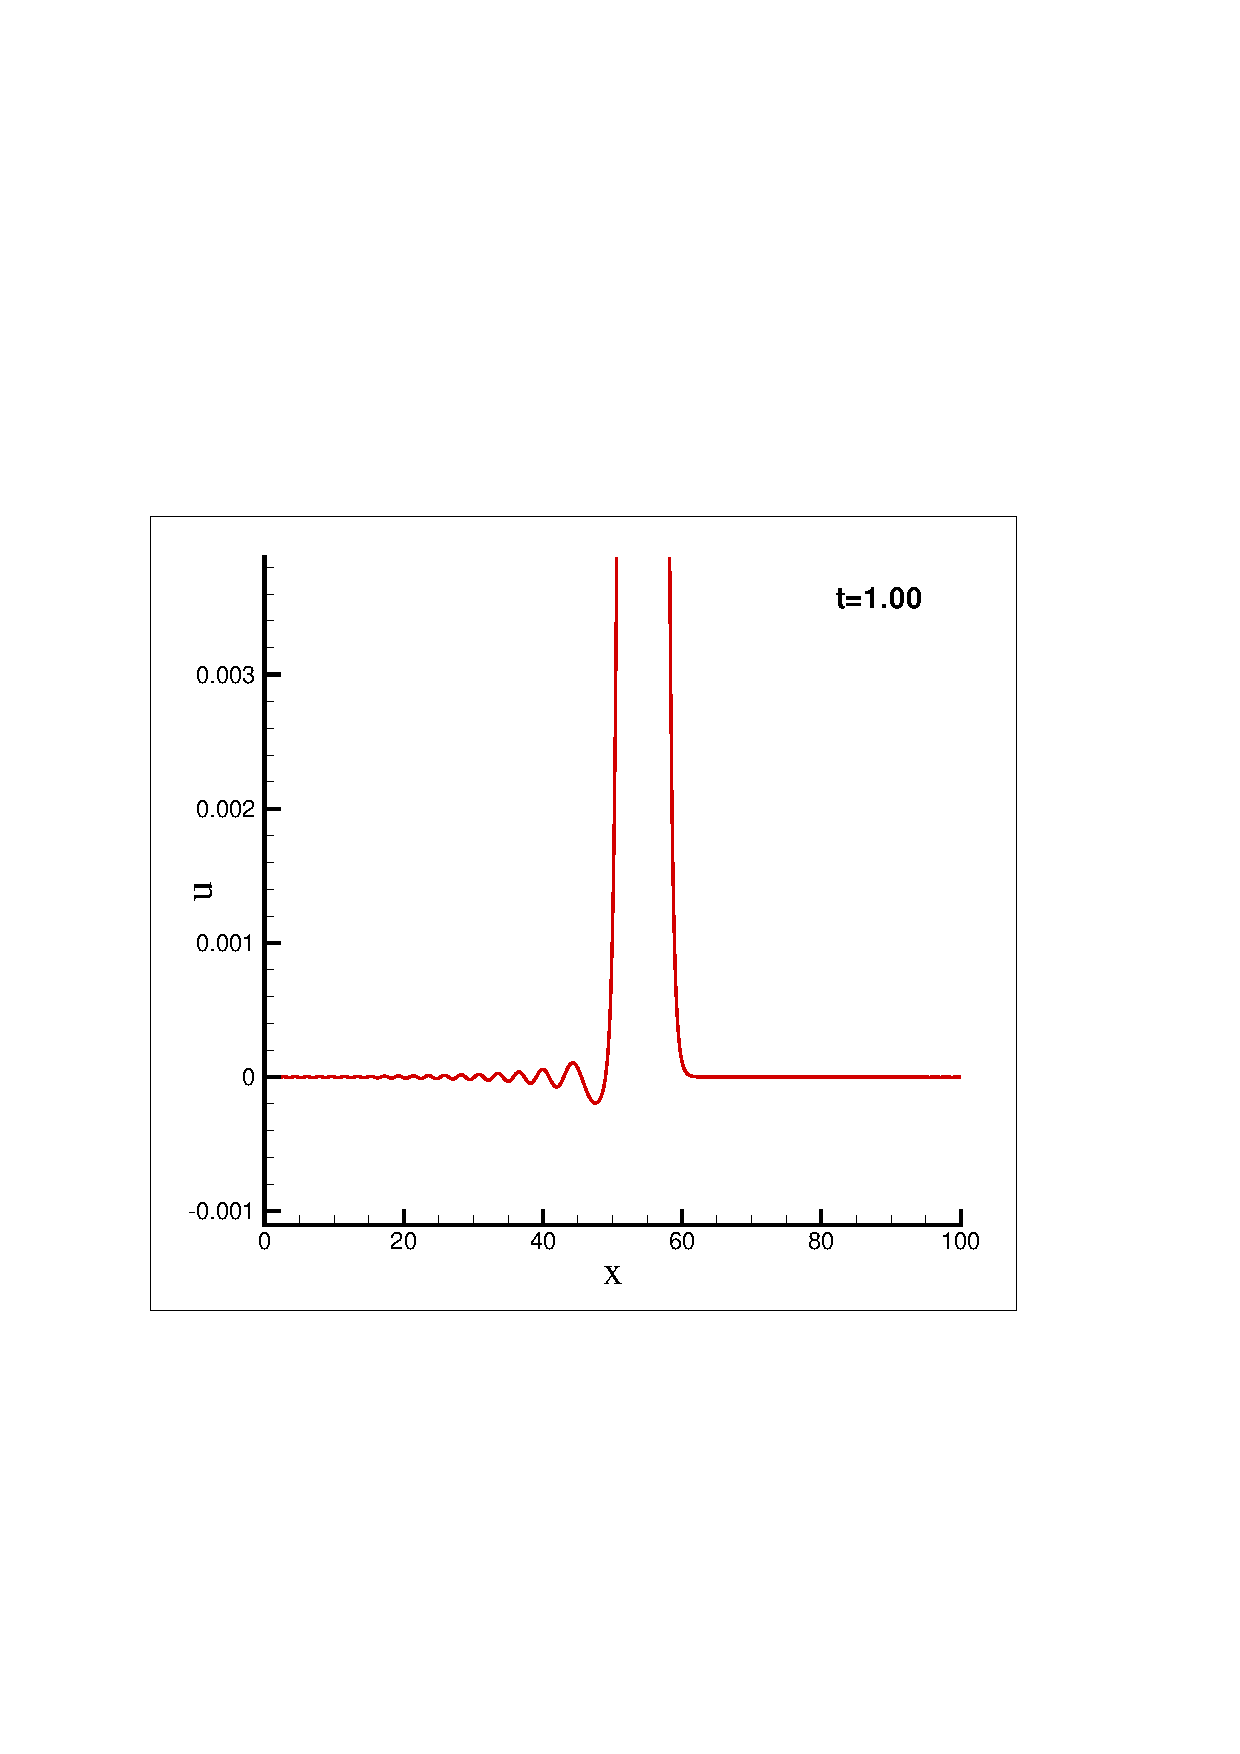
\includegraphics[width=0.5\linewidth]{Fig_2a}
\includegraphics[width=0.5\linewidth]{Fig_2b}
}
\caption{Magnified profile of the solution near the foot of a soliton demonstrating presence of an upstream propagating dispersive wave for two different initial conditions. For the reflecting potential, $u(x,0)=1.999\sech^2(x-50)$ shown in left frame and the reflectionless potential, $u(x,0)=2.000\sech^2(x-50)$ shown in right frame.}
\label{fig:reflect}
\end{figure}

\begin{figure}[h!]
\centerline{
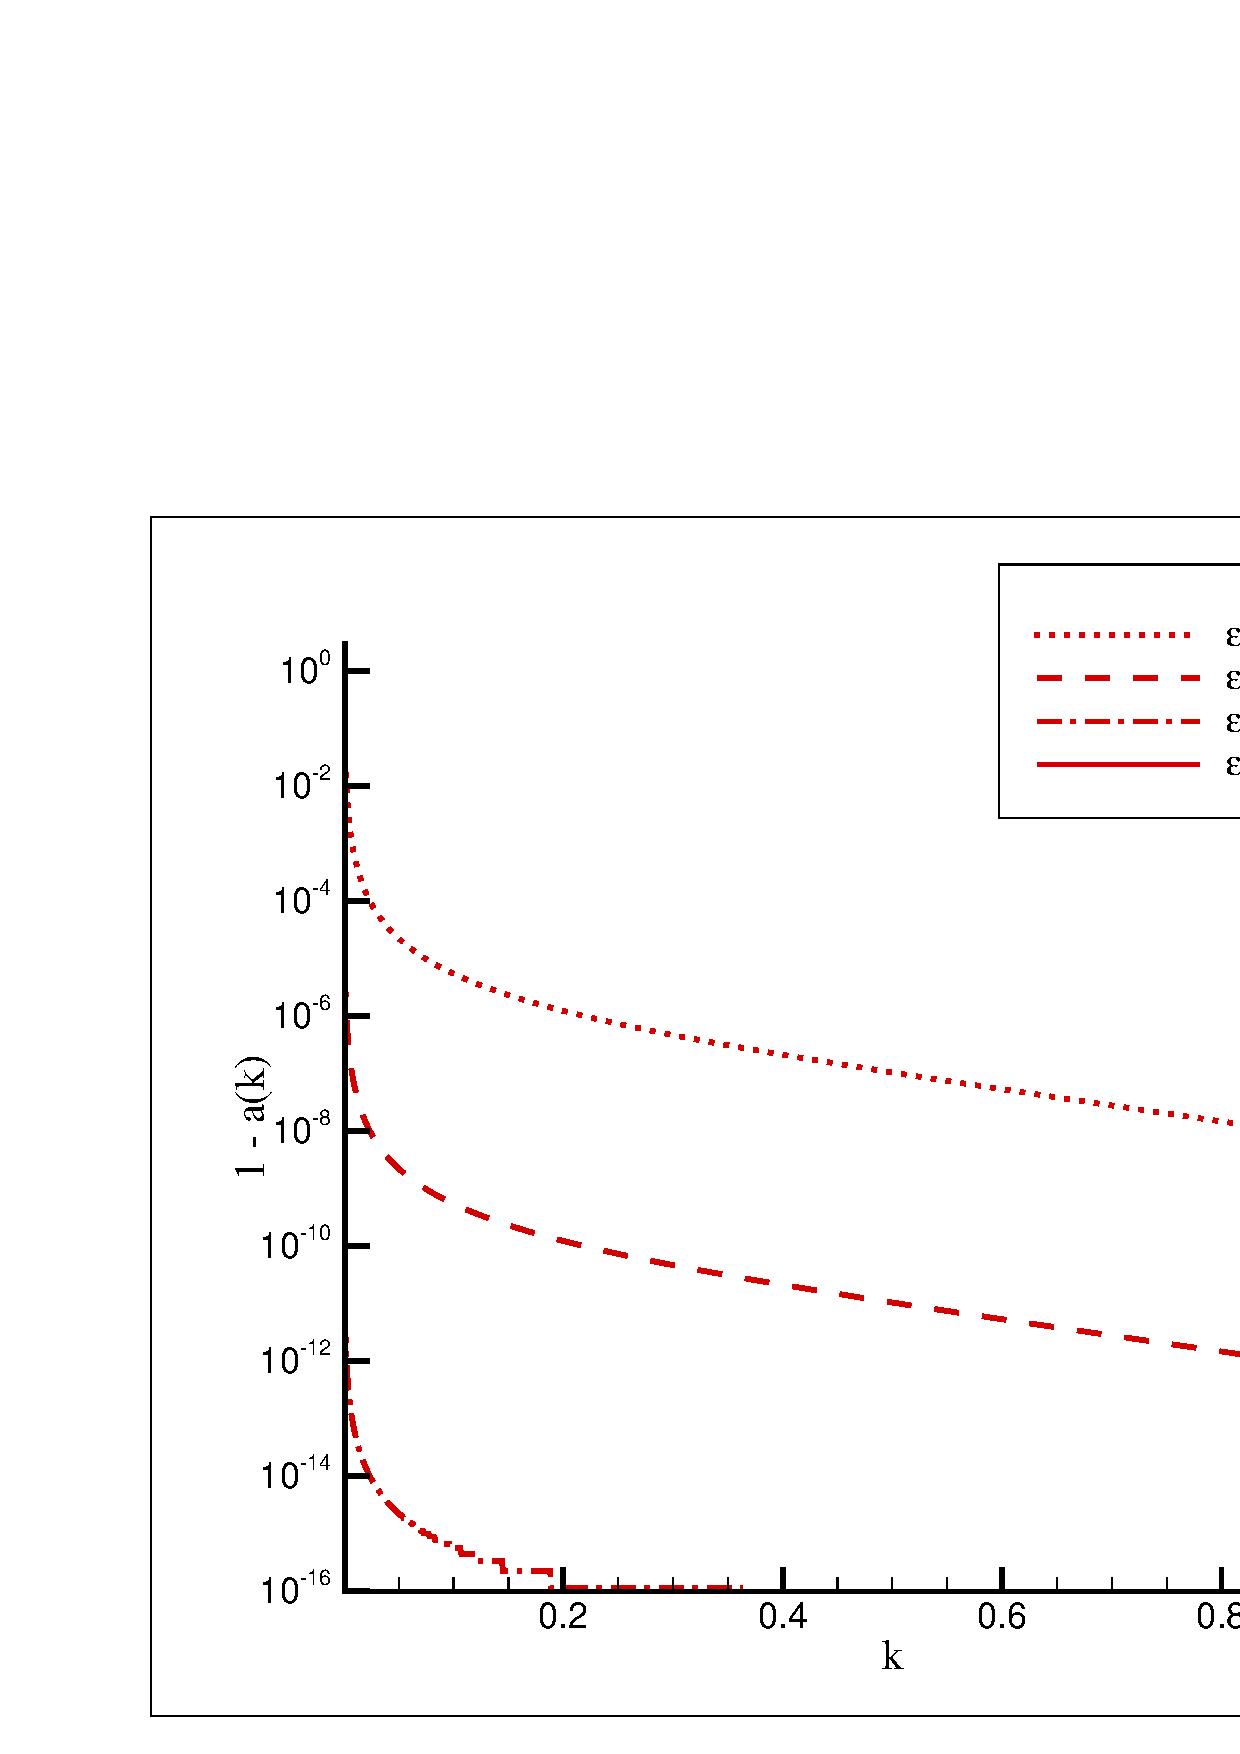
\includegraphics[width=0.5\linewidth]{Fig_3a}
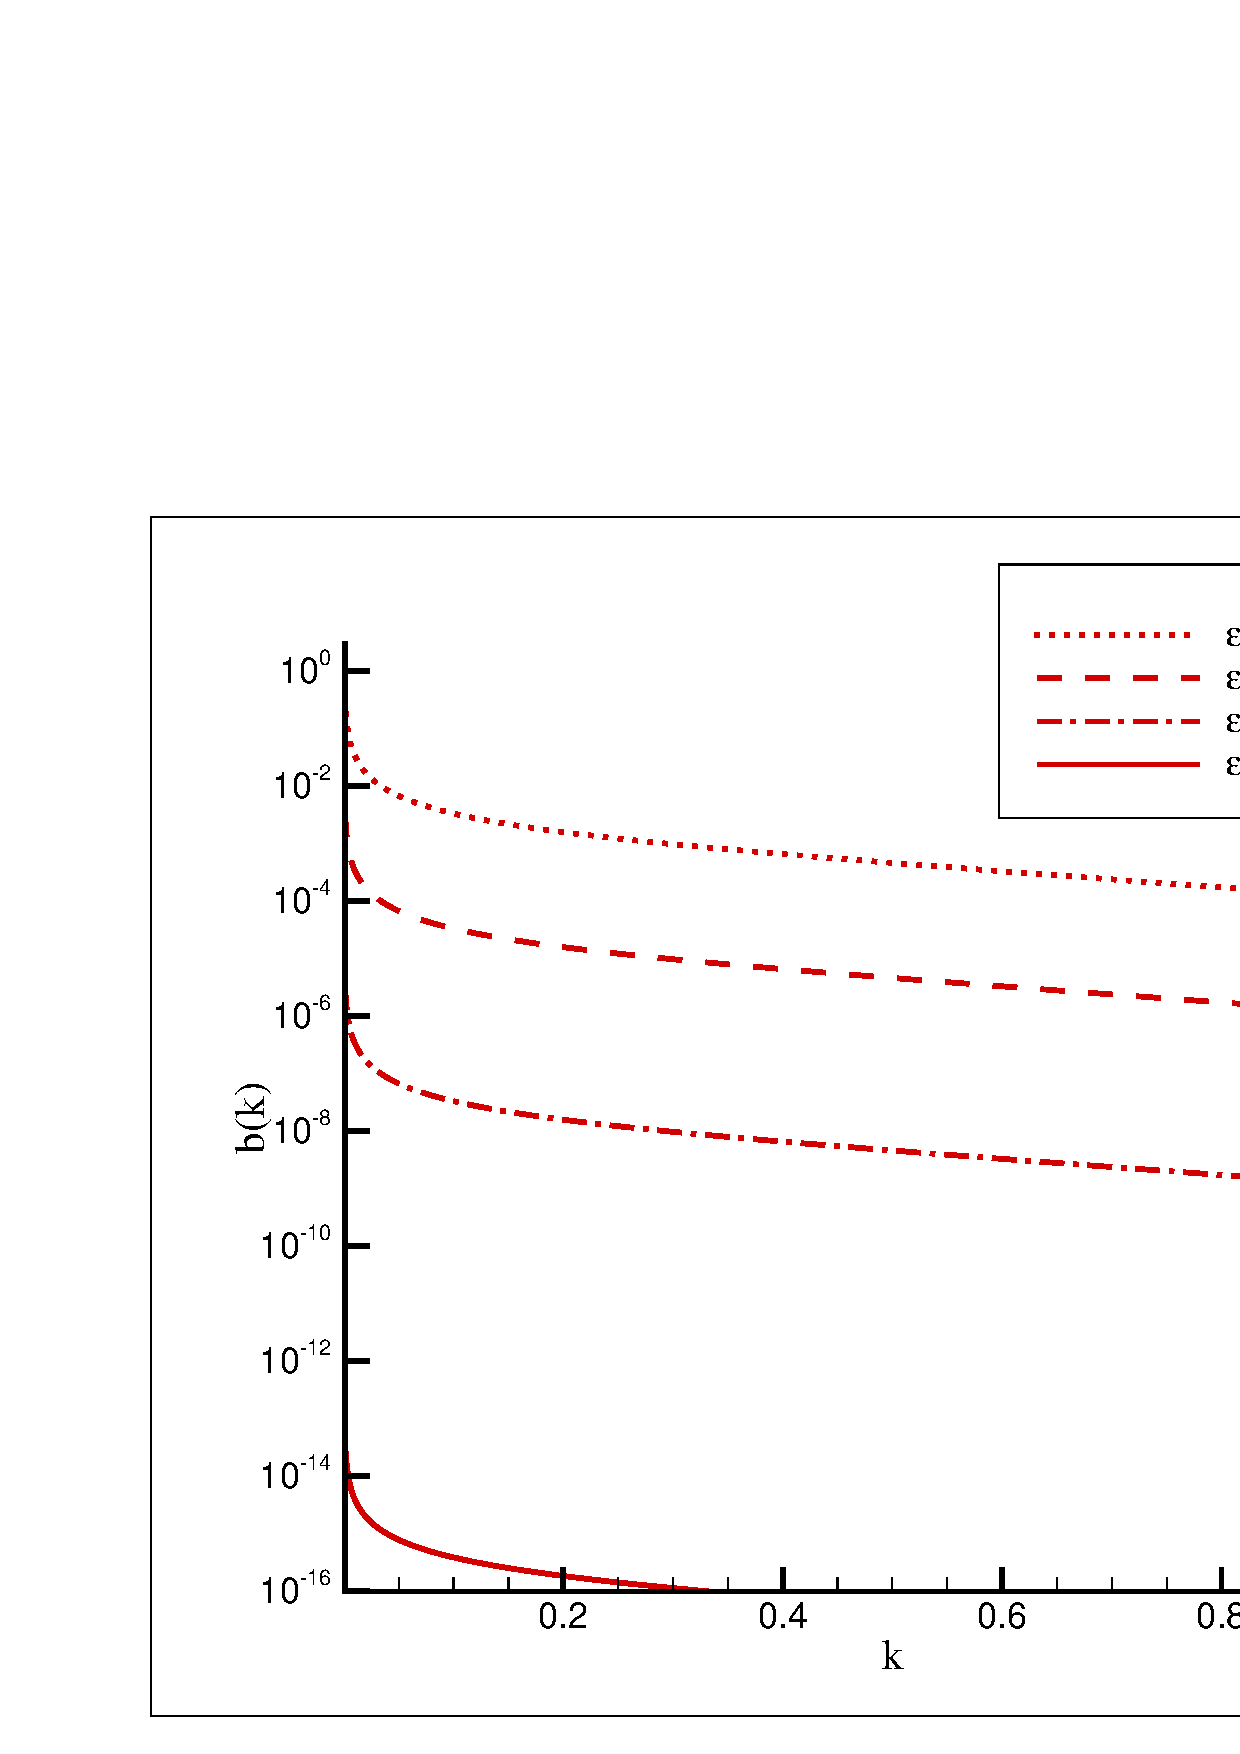
\includegraphics[width=0.5\linewidth]{Fig_3b}
}
\caption{Scattering coefficients computed based on different error levels in the initial condition, $u_0=(2 \pm \epsilon)\sech^2x$.}
\label{fig:akbk}
\end{figure}

It may be inferred from Eq. \eqref{eq:ao_n_relation} that, while computing the KdV equation, if one is able to retain the amplitude as close to $A_0 = N(N+1)$ as possible, one could reduce Gibbs' phenomenon. Any deviation from this amplitude would trigger upstream propagating dispersive waves. The amplitude of a numerical solution can be represented as
$$ A_N = A_0 \pm \epsilon $$
where $\epsilon$ represent the deviation in initial amplitude or some subsequent error arising as an effect of round-off, truncation and other sources. This deviation percolates into the solution in the form of transmitted and reflected waves, due to shift from the ideal values of the scattering coefficients for a reflectionless potential, $a(k)=1,b(k)=0$. In Fig. \ref{fig:akbk}, the error accounted in $a(k)$ and $b(k)$ as a result of different values of deviation, $\epsilon$ has been shown. It is evident that closer $A_0$ is to $N(N+1)$, smaller and negligible will be the reflected component 
of the solution. Also it should be noted that, as a result of the departure from the reflectionless profile given by $\epsilon$, the error in $b(k)$ is noticeably larger in magnitude in comparison to $1- a(k)$.

\begin{figure}[h!]
\centerline{
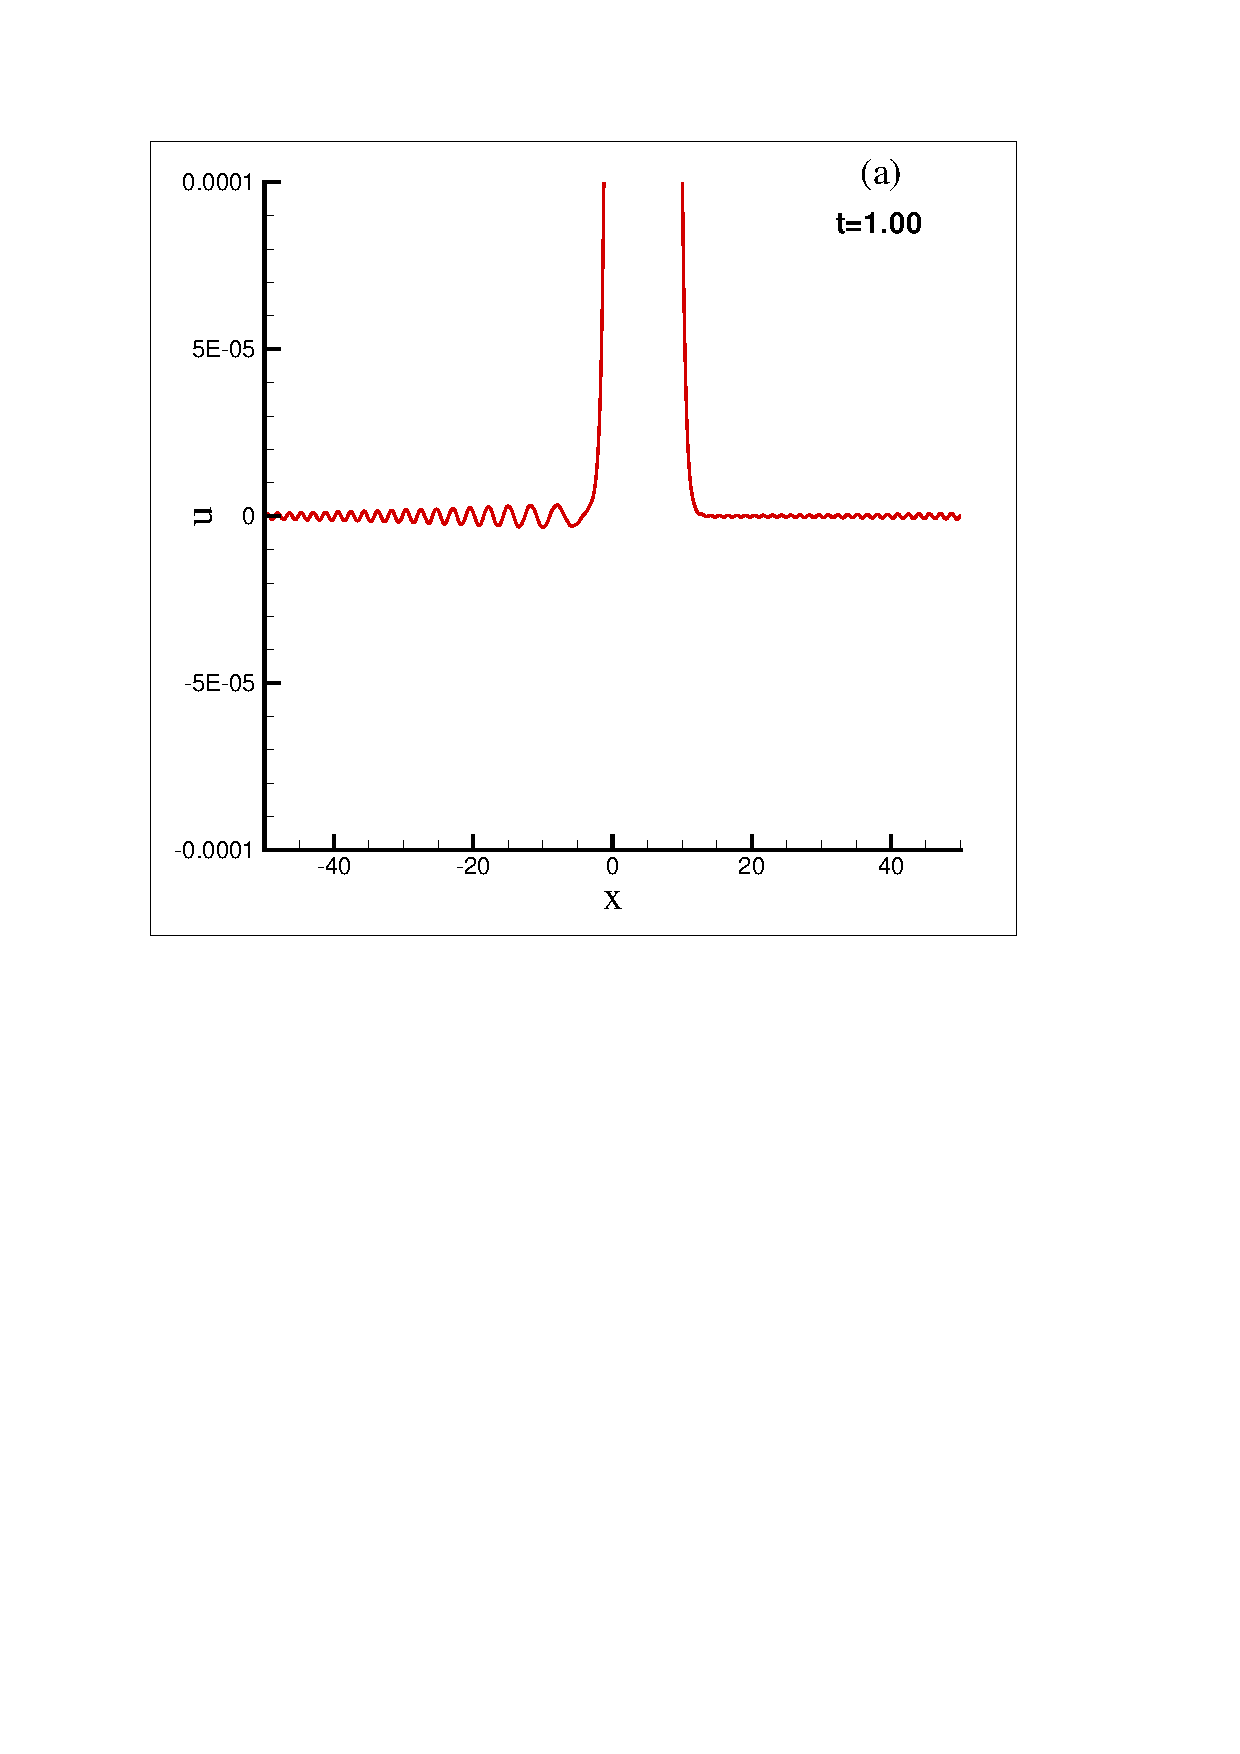
\includegraphics[width=0.33\linewidth]{Fig_4a}
\includegraphics[width=0.33\linewidth]{Fig_4b}
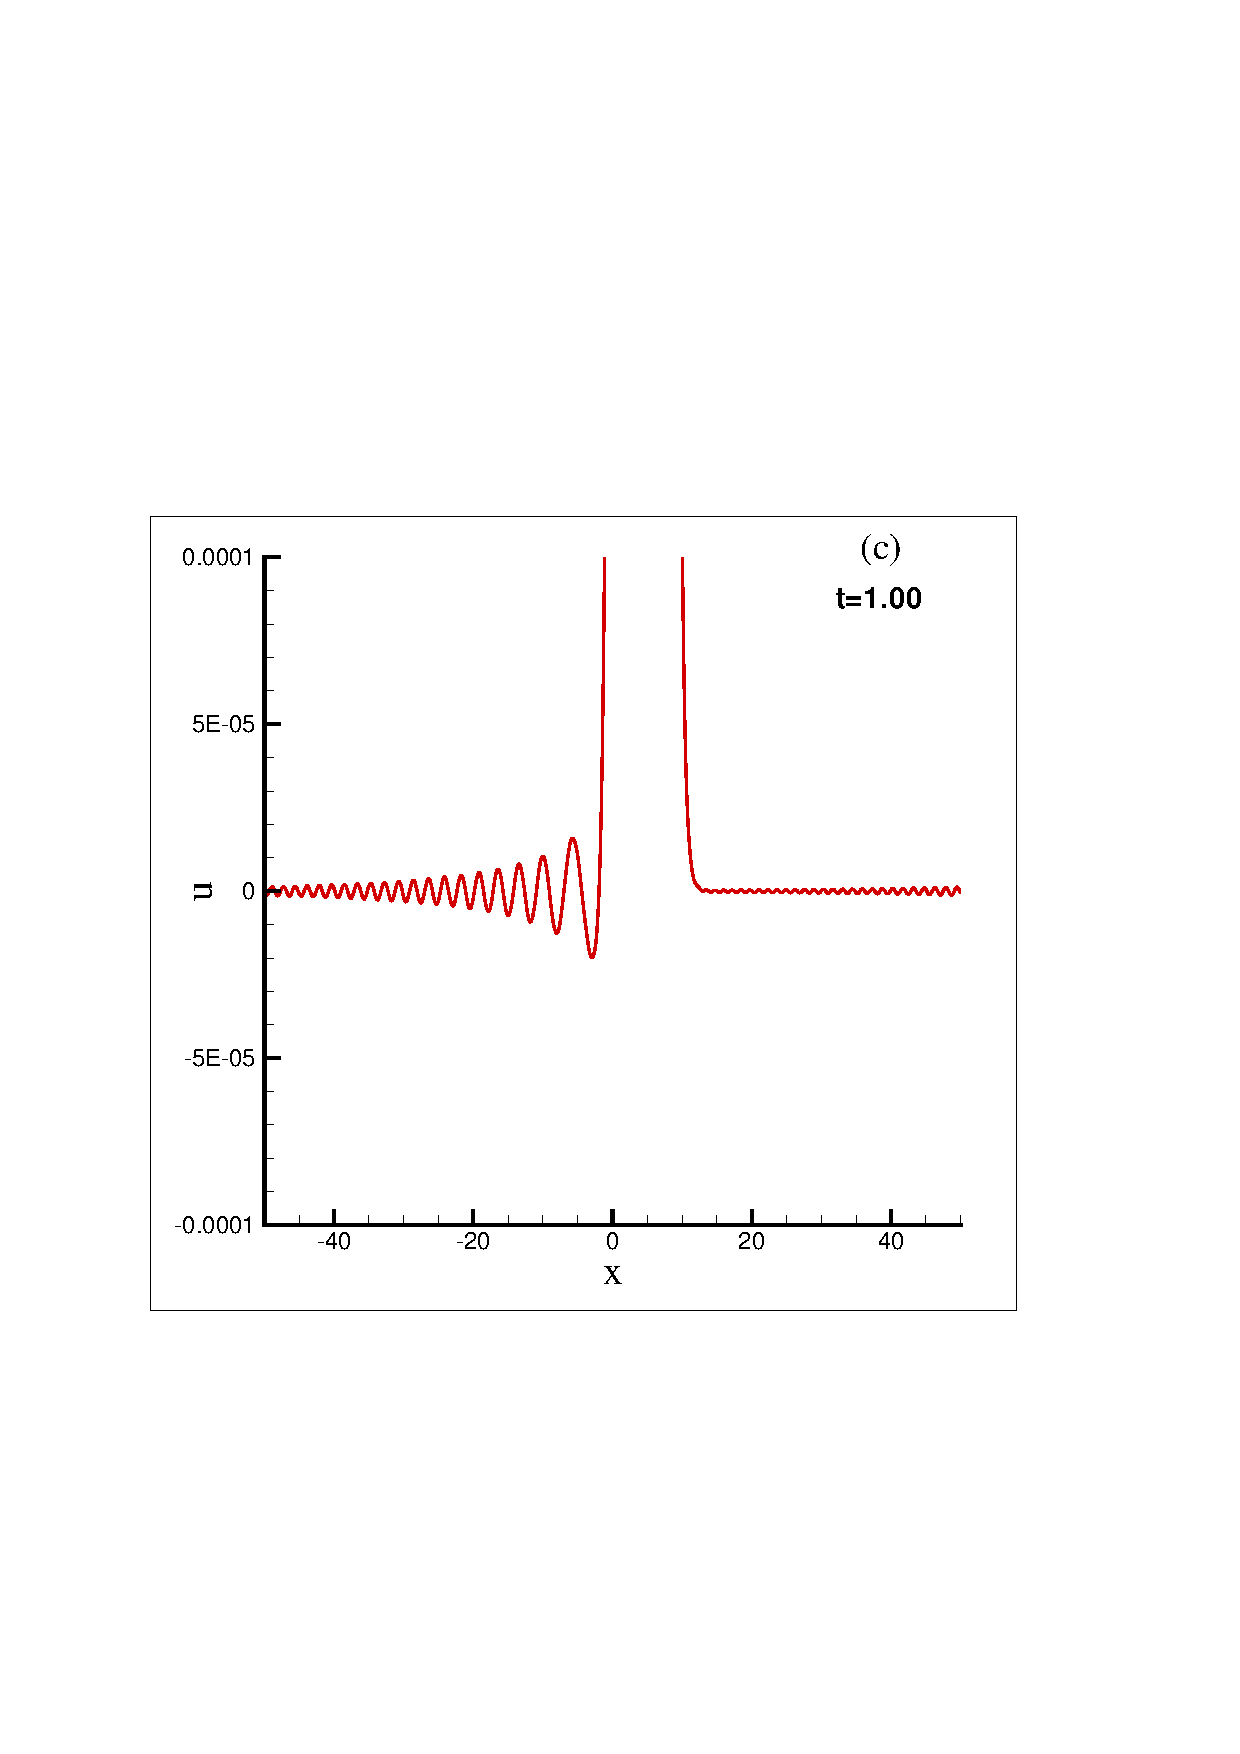
\includegraphics[width=0.33\linewidth]{Fig_4c}
}
\caption{Nature of dispersive wave, when computing with different schemes for $u_{xxx}$, starting from initial condition $u(x,0)=2\sech^2x$ (a) Optimized compact scheme; (b) Hybrid CD4-OUCS3 scheme; (c) Li-Visbal scheme.}
\label{fig:reflect3}
\end{figure}
The dispersive waves in a periodic domain tend to nonlinearly interact with the solitons and contaminate the solution. Ideally, for a reflectionless potential such waves should not exist. But a poorly resolved or dispersive numerical method also induce such waves, even at very early stages of the simulation. As shown in Fig. \ref{fig:reflect3}, the amount of reflection induced into the numerical solution is also dependent on the method used. 
Such reflected waves or Gibbs' phenomenon can be controlled, only with high resolution, neutrally stable and non-dispersive methods. In the present investigation, three such numerical schemes have been used for the solution of KdV equation. The design and numerical properties of these schemes are 
described in the following.

%-----------------------------------------------------------------------------------------------------
\section{Numerical Schemes}
\label{sec:num_sch}
Spatial discretization using finite difference methods can be broadly classified into two, i.e., explicit and implicit methods. In explicit methods, derivatives at any given node is calculated using an explicit expression in terms of the unknown. For better resolution and accuracy, higher order explicit methods may be used, which require larger stencils. Whereas in implicit methods, the derivatives are calculated by solving a linear system of equations. Within the family of implicit methods, compact schemes provide near-spectral accuracy with a compact stencil \cite{Sengupta2013a}. Therefore, for evaluating spatial derivatives in KdV equation for the convection and dispersion terms, following compact schemes have been adopted. In all the reported simulations, time integration of the KdV equation is done by classical four-stage, fourth-order Runge-Kutta method.

%-----------------------------------------------------------------------------------------------------
\subsection{Discretization of First Derivative or Convection Term}
\label{subsec:OUCS3}
The nonlinear convection term has been treated as a single quantity in the conservation form, as shown in Eqs. \eqref{eq:ckdv1} and \eqref{eq:ckdv2}. 
In this study, this term has been discretized using an optimized upwind compact scheme described in \cite{Sengupta2013a} as OUCS3 scheme. This is a 
compact scheme, which provides excellent spectral resolution, as shown in \cite{Sengupta2006b}. The first derivative is evaluated by solving a linear system of equations for the whole domain given by
$$ [A]\{u'\} = [B]\{u\} $$
All compact schemes utilize Pad\'e approximation for differential equations. A three point stencil for $[A]$ and central five point stencil for $[B]$ are used, which can be evaluated using tridiagonal matrix algorithm (TDMA):

\begin{equation}
\label{eq:oucs3}
\alpha_{-1}u_{j-1}^{\prime}+u_{j}^{\prime}+\alpha_{1}u_{j+1}^{\prime}=\frac{1}{h}[a_{2}u_{j+2}+a_{1}u_{j+1}+a_{0}u_{j}+a_{-1}u_{j-1}+a_{-2}u_{j-2}]
\end{equation}
where,
\begin{align*}
\alpha_{\pm1}=D\pm\frac{\eta}{60},\
a_{\pm2}=\pm\frac{F}{4}+\frac{\eta}{300},\
a_{\pm1}=\pm\frac{E}{2}+\frac{\eta}{30},\ a_{0}=-\frac{11\eta}{150}\\
D=0.3793894912,\
E=1.57557379,\
F=0.183205192
\end{align*}

 To retain the central nature of spatial discretization and thus, to avoid numerical diffusion the upwinding parameter, $\eta$ is set as zero \cite{Sengupta2013a,Sengupta2006b}.
%-----------------------------------------------------------------------------------------------------
\subsection{Discretization of Third Derivative or Dispersion Term}
The third derivative rarely occurs in fluid dynamical simulations. Here we describe two alternative novel methods for the discretization of the third derivative, along with another third derivative compact scheme reported in \cite{Li2006}. Before we describe the methodology behind developing these schemes and its numerical properties, the stencils of these finite difference schemes have been introduced below.

The first one is an \textit{optimized compact scheme} which calculates the third derivative from an implicit stencil given by,
\begin{equation*}
\label{matrix}
[A_1]\{u'''\} = [B_1]\{u\}
\end{equation*}
which for a general node is given by a five-point stencil,
\begin{equation}
\label{pade}
\alpha u_{j-1}^{'''} +  u_{j}^{'''} + \alpha u_{j+1}^{'''} 
= \frac{\bar{a}}{2h^3}\left[u_{j+1}-u_{j-1}\right] + \frac{\bar{b}}{16h^3}\left[u_{j+2}-u_{j-2}\right]
\end{equation}
The values of the coefficients in Eq. \eqref{pade} are $\alpha=0.477022022$; $ \bar{a}= -4\alpha-2;\; \bar{b}=16\alpha +8$ obtained through an optimization procedure described in the following section. 

Secondly, a \textit{hybrid scheme} has been developed using the fourth order central difference (CD4) scheme for the second derivative, which is differentiated again by OUCS3 scheme to obtain the third derivative. The second derivative is evaluated using the following stencil for CD4

\begin{equation}
\label{eq:cd4}
u_{j}^{\prime\prime}=\frac{-u_{j+2}+12u_{j+1}-30u_{j}+12u_{j-1}-u_{j-2}}{12h^{2}}
\end{equation}

Another compact scheme was reported and applied to the KdV equation in \cite{Li2006}. This scheme, hitherto referred to as the \textit{Li-Visbal scheme}, employs a seven-point stencil to evaluate the third derivative, in comparison to the scheme given in Eq. \eqref{pade}. This is given by,
\begin{equation}
\begin{aligned}
\label{eq:pade_li}
\alpha_1 u_{j-1}^{'''} +  u_{j}^{'''} + \alpha_1 u_{j+1}^{'''} 
= \frac{a_1}{2h^3}\left[u_{j+2}-2u_{j+1}+2u_{j-1}- u_{j-2}\right] \\
+ \frac{b_1}{8h^3}\left[u_{j+3}-3u_{j+1}+3u_{j-1}- u_{j-3}\right]
\end{aligned}
\end{equation}
The values of the constants in the above stencil, were set by matching Taylor's series expansions on either sides of equation, obtained as 
$\alpha_1 = 7/16,\,a_1= 2,\,b_1=-1/8$. 

\subsubsection{Optimized Compact Scheme for Third Derivative}
\label{subsec:OCS}
Compact schemes are known to be superior in resolution and in preserving dispersion relation properties for model linear convection equation. The procedure for designing a compact scheme to evaluate the first derivative has been elaborated in \cite{Sengupta2013a,Sengupta2006b}. The same procedure can be employed to calculate the third derivative. An implicit linear system of equations is formed to compute the derivatives in the domain from known function values at each nodes as $[A_1]\{u'''\} = [B_1]\{u\}$.

The stencil of this implicit scheme is given by Eq. \eqref{pade}. One notes that all even derivatives are absent from Eq. \eqref{pade} after Taylor's series expansion. The following equations are obtained by 
equating the odd derivatives.
\begin{align}
\label{eq:taylor1}
u_{j}^{'}   &:&  4\bar{a} + \bar{b}&=0 \\
\label{eq:taylor3}
u_{j}^{'''} &:  & \bar{a} + \bar{b} - 12\alpha&=6\\
\label{eq:taylor5}
u_{j}^{v}   &:   &\bar{a} +4\bar{b} -120\alpha&=0
\end{align}
Equations \eqref{eq:taylor1} and \eqref{eq:taylor3} are the required consistency conditions for proper representation of third derivative. Solving Eqs. \eqref{eq:taylor1} to \eqref{eq:taylor5} simultaneously, yields the solution $\alpha = 0.5$ for the resultant sixth order scheme. The procedure to characterize any general finite difference scheme has been shown in \cite{Sengupta2003b}, following which the numerical third derivative is represented as: $u'''_j = \int ik_{eq}^{(3)}\hat{U}(k)e^{ikx_j}dk$. Using this, the normalized resolution of the aforementioned compact scheme is given by
\begin{equation}
\label{keq}
- \frac{k_{eq}^{(3)}}{k^3} = - \frac{8\bar{a} \sin(kh)+\bar{b}\sin(2kh)}{8(kh)^3[1+2\alpha\cos(kh)]}
\end{equation}
For the sixth order scheme for which $\alpha = 0.5$, Eq. \eqref{keq} reduces to
\begin{equation}
\label{keq1}
- \frac{k_{eq}^{(3)}}{k^3} = \frac{4\sin(kh)}{(kh)^3} \tan^2\left(\dfrac{kh}{2}\right)
\end{equation}
This implies the resultant sixth order scheme may not necessarily be the most accurate representation of the third derivative, as $\alpha = 0.5$ results in a compact scheme which behaves poorly in the high wavenumber limit: $kh\to\pi$, with $- {k_{eq}^{(3)}}/{k^3} \to \infty$.
%However, this may not necessarily the most accurate representation of the third derivative, as for $\alpha = 0.5$ we have a compact scheme which behaves poorly in the high wavenumber limit: $kh\to\pi$.

 As explained in \cite{Sengupta2013a,Sengupta2006b}, spectral resolution of the discretization
can be improved by releasing the order of accuracy of the method, by floating one of the constants in Eqs.  \eqref{eq:taylor1} and \eqref{eq:taylor3}
and optimizing the resultant lower order scheme. Thus, the scheme is modified by satisfying the consistency condition, Eqs. \eqref{eq:taylor1} and 
\eqref{eq:taylor3}, while using $\alpha$ as a floating parameter to minimize error of representation of the derivative. The parametric equations for 
$\bar{a}$ and $\bar{b}$ in terms of $\alpha$ are: $ \bar{a}= -4\alpha-2;\; \bar{b}=16\alpha +8$. The scheme is then optimized by estimating the following objective function for different values of $\alpha\; \epsilon\; (0,0.5)$ and minimizing it
\begin{equation}
\label{obj}
I(\alpha) = \int_0^{\gamma\pi} \left| 1 - \frac{-k_{eq}^{(3)}}{k^3} \right| dkh
\end{equation}
with $0<\gamma\leq 1$, by estimating the error in a reduced range of maximum wavenumber ($kh = \pi$). The optimum value of $\alpha$ was obtained as 
$\alpha=0.477022022$ for $\gamma = 0.50$, as shown in Fig. \ref{fig:optim} for $I(\alpha)$. This optimal $\alpha$ reduces discretization error of the dispersion term in KdV equation, as shown later in section \ref{sec:res}. 

\begin{figure}[h!]
\center
\includegraphics[width=0.5\linewidth]{Fig_5}
\caption{Optimization of the compact scheme by evaluating the objective function against $\alpha$.}
\label{fig:optim}
\end{figure}

In the following, we describe a hybrid method composed of explicit and implicit schemes, which is strictly central and is chosen as a compromise between efficiency (provided by explicit method) and accuracy (provided by implicit
method). 


%-----------------------------------------------------------------------------------------------------
\subsubsection{Hybrid CD4-OUCS3 for Third Derivative}
While solving the KdV equation, one can adopt the governing equation in the conservation form, represented by Eq. \eqref{eq:ckdv1}. In this approach the convection and the dispersion terms in Eq. \eqref{eq:ckdv1} are calculated together as $\left(3 u^2 + u_{xx,CD4}\right)_{x,OUCS3}$. The stencil for CD4 and OUCS3 are given by Eqs. \eqref{eq:cd4} and \eqref{eq:oucs3} respectively. In this approach, OUCS3 is applied only once, and thus, it requires only one compact scheme to be evaluated; whereas the other methods reported here utilizes two separate compact schemes for convection and dispersion terms. Hence, the computational cost is considerably less for applying the hybrid scheme.

The resolution for this hybrid scheme in representing the third derivative is given by
\begin{equation}
\begin{aligned}
-\frac{k_{eq}^{(3)}}{k^{3}}=-\frac{1}{24(kh)^{3}(1+2D \cos{kh})} \bigl[ 2E\left(-\sin(3kh)+16\sin(2kh)-29\sin(kh)\right)\\
                            + F\left(-\sin(4kh)+16\sin(3kh)-30\sin(2kh)+16\sin(kh)\right)\bigr]
\end{aligned}
\end{equation}

The values of the coefficients $D,E$ and $F$ are the same as described earlier in subsection \ref{subsec:OUCS3}.

The advantage of using a mix of explicit and implicit schemes to evaluate the spatial derivatives clearly shows up in terms of spectral resolution. This scheme performs remarkably well, as illustrated in Fig. \ref{fig:keq}, in comparison with conventional explicit schemes such as, second order (CD2) and fourth order (CD4) central difference schemes for the third derivative given by
\begin{align}
u^{\prime\prime\prime}_{j,CD2}&=\frac{u_{j+2}-2u_{j+1}+2u_{j-1}-u_{j-2}}{2h^{3}}\\
u^{\prime\prime\prime}_{j,CD4}&=\frac{-u_{j+3} +8u_{j+2} - 13u_{j+1} + 13u_{i-1} - 8u_{j-2} + u_{j-3}}{8h^3}
\end{align}

\begin{figure}[h!]
\centerline{
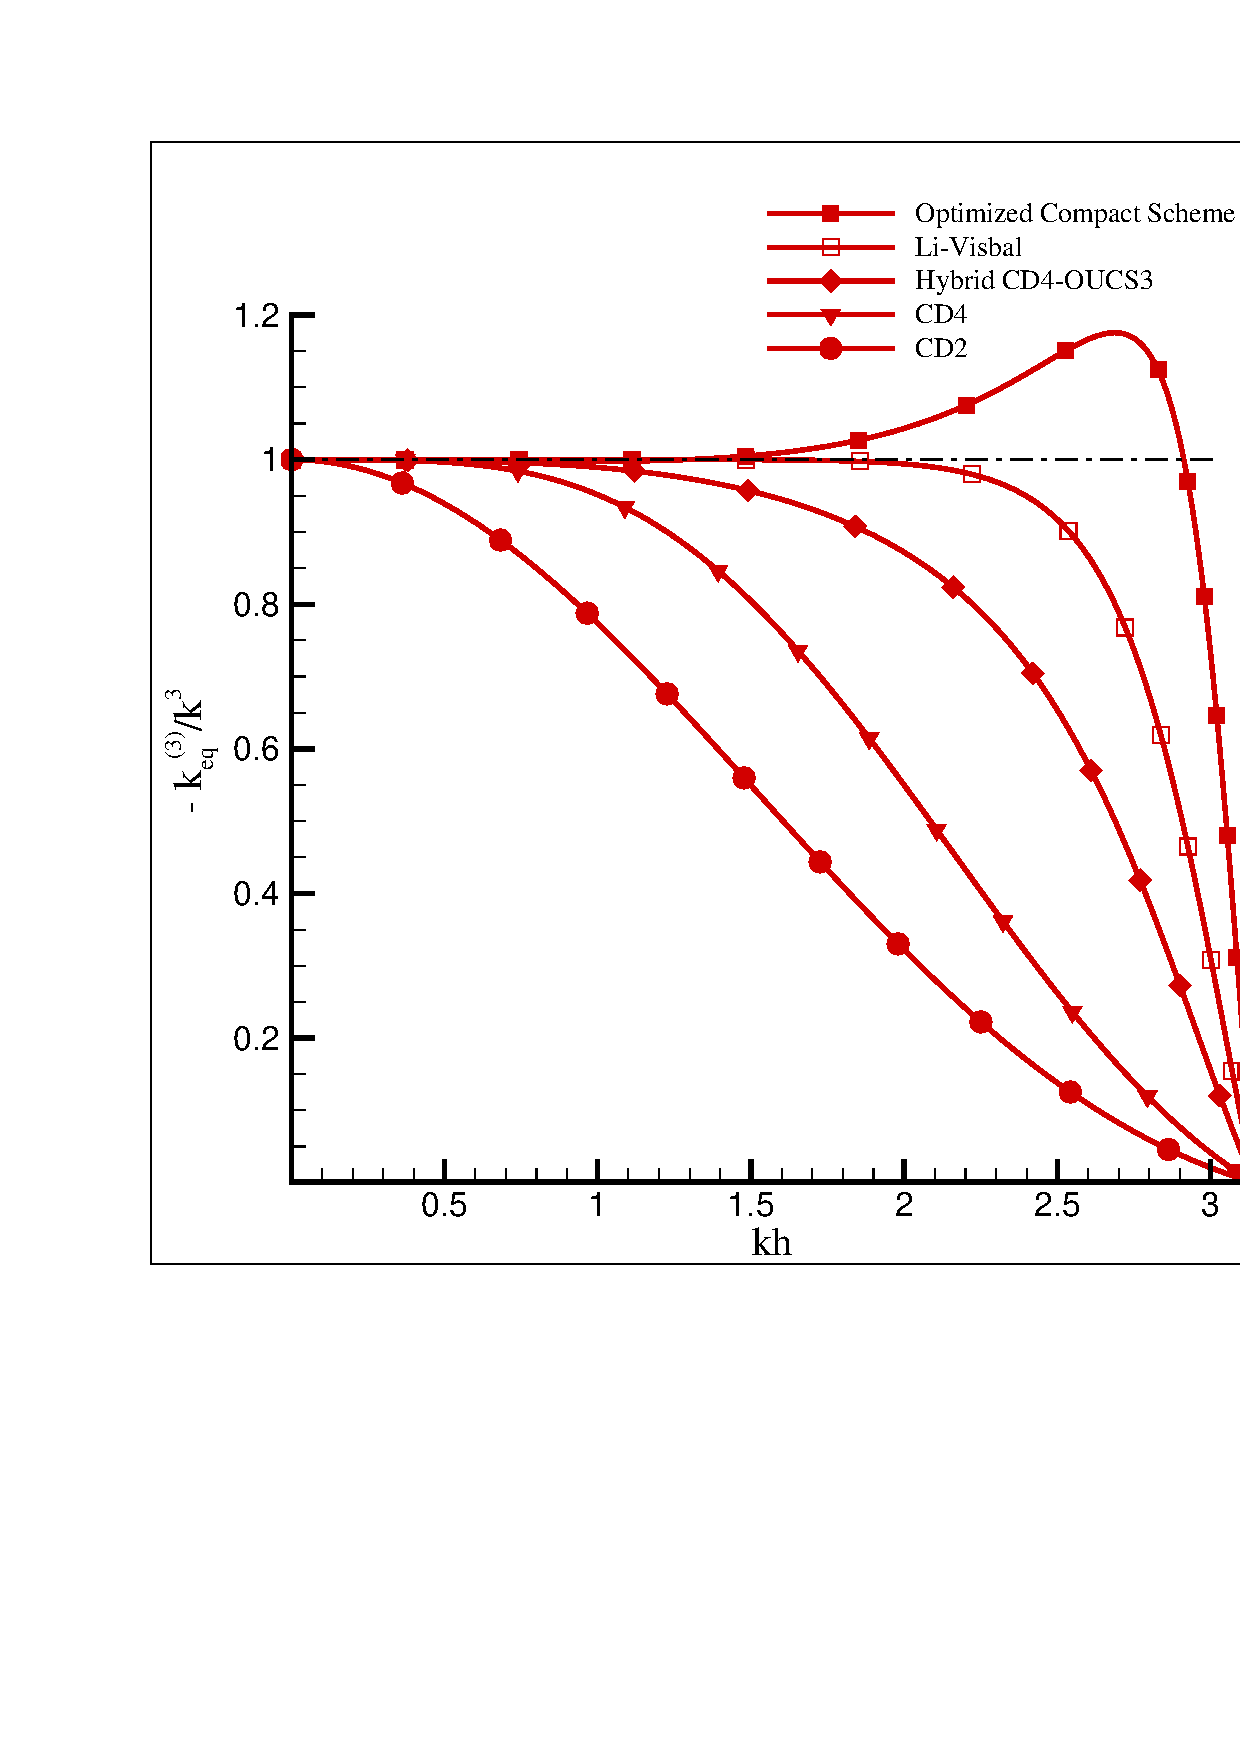
\includegraphics[width=0.5\linewidth]{Fig_6}
}
\caption{Spectral resolution of various third derivative schemes plotted against non-dimensional wavenumber, $kh$.}
\label{fig:keq}
\end{figure}

Figure \ref{fig:keq} also displays the resolution of the optimized compact scheme for third derivative and another scheme due to \cite{Li2006}, which 
is described next.

%-----------------------------------------------------------------------------------------------------
\subsubsection{Li-Visbal scheme for Third Derivative}
This is a \emph{sixth order} accurate implicit scheme for calculating the third derivative. The stencil for this compact scheme is given by Eq. \eqref{eq:pade_li}. It can be shown that by putting $b_1=0$ in Eq. \eqref{eq:pade_li} and by optimizing the scheme, one would recover the optimized compact scheme used in this work. Since this scheme has adopted a larger stencil, and satisfies Taylor's series till the eighth derivative term $u^{viii}$, this compact scheme has better spectral resolution compared to other schemes shown in Fig. \ref{fig:keq}, except the optimized compact scheme. The resolution of this scheme is given by 
\begin{equation}
\label{eq:keq_li}
-\frac{k_{eq}^{(3)}}{k^{3}}=
      -\frac{4a_1\left[2\sin(2kh) - 4\sin (kh)\right] + b_1\left[2\sin(3kh)- 6\sin (kh) \right]}
           {8(kh)^3 (1+2\alpha_1\cos kh) }
\end{equation}

%-----------------------------------------------------------------------------------------------------
\section{Error dynamics of One-Dimensional Dispersion Equation} 
\label{sec:err}
It is important to obtain the numerical properties of discretization schemes used in solving an equation. In \cite{Fornberg1978}, a linear stability analysis was done on a linear convection-dispersion equation to fix the limits of time-step and mesh size for solving the KdV equation. For the one-dimensional convection equation in \cite{Sengupta2007}, a complete space-time dependent error analysis was reported for different combinations of time integration methods and schemes used for first derivative. A similar approach is used here for the chosen model equation involving a third derivative 
used in \cite{Li2006,Yan2002}.
\begin{equation}
\label{eq:disp_eqn}
u_t + c^{-2}u_{xxx} = 0
\end{equation}

The initial condition and the corresponding exact solution are $u(x,0)=\sin(cx);$ $u(x,t)=\sin[c(x+t)]$, respectively. The exact solution $u(x,t)$ can be represented  by its Fourier-Laplace transform as 

\begin{equation*} 
u(x,t) = \int \int \hat{U}(k, \omega)  \hspace{1mm} e^{i(kx-\omega t)} dk 
\hspace{1mm} d{\omega}
\end{equation*}
using which the dispersion relation for Eq. \eqref{eq:disp_eqn} is 
\begin{equation}
\label{eq:disp_rel}
\omega = -\frac{k^3}{c^2}
\end{equation}
From Eq. \eqref{eq:disp_rel}, the exact phase speed and the group velocity of the solution is given by, $c_{ph} = \omega/k= -k^2/c^2$, and 
$V_g = -3k^2/c^2$, respectively.

For any general discretization, the spatial derivative $u'''_j$ is evaluated as $\{u'''\} = \frac {1}{h^3} [C] \{u\}$. The matrix $[C]$ is constructed 
by the numerical scheme applied in the interior and for the near-boundary points, with the dimension of the matrix equal to the number of nodes. 
Therefore, the derivative at the $j^{th}$ node is evaluated as $u'''_j = \frac {1}{h^3} \sum_{l=1}^{N} C_{jl} u_l$, where $ u_l = u(x_l,t) = \int U(k,t)\; e^{i k x_l} dk$ is the value of the function at $l^{th}$ node and $N$ is the total number of nodes used for discretization. Using spectral representation, the numerical derivative is written as

\begin{equation} \label{3rd_der_num}
u'''_j = \int \frac{1}{h^3} \sum_{l=1}^N C_{jl} U(k,t) \hspace{1mm} e^{i k (x_l-x_j)} e^{i k x_j} dk
\end{equation}
Thus, Eq. \eqref{eq:disp_eqn} can be expressed in the spectral plane as 

\begin{equation}
\int \left[ \frac {d U}{d t} + \frac {1}{c^2h^3} \sum_{l=1}^N U C_{jl}
     e^{i k x(x_l-x_j)} \right] e^{i k x_j} dk = 0
\end{equation}
The integrand of the above must be zero for all wavenumbers, which implies,
\begin{equation}
\frac{dU}{U} = - N_d \sum \limits_{l=1}^{N} C_{jl} e^{i k (x_l-x_j)} = -A_j
\end{equation}
where, $N_d = \Delta t/(c^2h^3)$ is a non-dimensional number characterizing dispersion, analogous to Courant-Friedrich-Lewy number and Peclet number used for numerical solution of hyperbolic and parabolic PDEs, respectively. The numerical amplification factor for time integration can be defined as
\begin{equation*}
G_j = \frac{U(k,t + \Delta t)}{U(k,t)} 
\end{equation*}

The error propagation equation for Eq. \eqref{eq:disp_eqn} is obtained following the method in \cite{Sengupta2007} as 

\begin{equation} 
\label{eq:epe1}
\frac{\partial e}{\partial t} + \frac{1}{c^2} \frac{\partial^3 e}{\partial x^3} =\frac{\partial (u-u_N)}{\partial t} + \frac{1}{c^2} \frac{\partial^3 (u-u_N)}{\partial x^3} 
\end{equation}

By the governing equation, the right hand side (RHS) is equivalent to 
$-(\frac{\partial u_N}{\partial t} + \frac{1}{c^2} \frac{\partial^3 u_N}{\partial x^3}),$
where $u_N$ is the numerical solution. Representing the initial condition by its Laplace transform, $ u_N(x_j,t=0) = \int U_0(k)\; e^{i k x_j} dk$, 
the numerical solution at any instant can be expressed as 
\begin{equation}
\label{eq:un1}
u_N(x_j,n\Delta t) = \int U_0(k)\; |G_j|^n\; e^{i(kx_j - n\beta_j)} dk
\end{equation}
$G_j$ is the numerical amplification factor, which being a complex quantity can also be represented as $G_j = |G_j|e^{-i\beta_j}$. By using the 
numerical dispersion relation for a general wave solution, $\omega_N = kc_N$, where $c_N$ is the numerical phase speed, we can relate the phase of 
the numerical amplification factor to the phase of the numerical solution, i.e., $n\beta_j = \omega_N t=kc_Nt$. Thus, Eq. \eqref{eq:un1} can be 
rewritten as
\begin{equation}
\label{eq:un2}
u_N(x_j,n\Delta t) = \int U_0(k) |G_j|^n e^{ik(x_j - c_Nt)} dk
\end{equation}
Using this representation, the terms in the RHS of Eq. \eqref{eq:epe1} can be expressed as
\begin{align}
\label{eq:unt}
\frac{\partial u_N}{\partial t}
  = &\int \left( \frac{ln|G_j|}{\Delta t}  -ikc_N \right)  U_0(k) |G_j|^n e^{ik(x_j - c_Nt)} dk\\
\label{eq:unx3}
\frac{\partial^3 u_N}{\partial x^3}
  = &\int -ik^3 U_0(k)\; |G_j|^n\; e^{ik(x_j - c_Nt)} dk 
\end{align}

Using Eqs.\eqref{eq:unt} and \eqref{eq:unx3} in Eq. \eqref{eq:epe1}, the error propagation equation simplifies to 

\begin{align}
\label{eq:epe2}
\begin{split}
&\frac{\partial e}{\partial t} + \frac{1}{c^2} \frac{\partial^3 e}{\partial x^3} \\
   = &-\int \frac{ln|G|}{\Delta t} U_0(k) |G_j|^n e^{ik(x_j - c_Nt)} dk 
     +\frac{1}{c^2}\left[1-\frac{c_N}{c_{ph}}\right]\frac{\partial^3 u_N}{\partial x^3}\\
     &- \int \frac{3}{kc^2}\left[\frac{c_N}{c_{ph}} - \frac{V_{gN}}{V_g}\right]\int -ik'^3 U_0(k') |G_j|^n e^{ik'(x_j - c_Nt)} dk' dk
     \end{split}
\end{align}

The RHS of Eq. \eqref{eq:epe2} identifies the sources of errors which affect the numerical solution. The first term on RHS is due to the numerical amplification factor, associated with numerical stability or instability. A scheme is neutrally stable when $|G_j| = 1$. The second term on RHS 
represents phase error, which affects the numerical solution strongly in the presence of large solution gradient. As in the case of KdV equation, 
the solitons are the sites of large higher order derivative values. Although this third derivative term determines dispersion, still it encapsulates 
the nonlinear effects due to dominance of the higher derivative term. The third term on RHS is also due to dispersion error, which signifies the 
deviation of numerical group velocity ($V_{gN}$) from the exact group velocity ($V_g$) and once again, is magnified by higher order derivatives of the solution. While the first term on RHS is due to the general numerical property of the method used, the other two terms on RHS 
show the effects of nonlinearity and is determined by the spectrum of the solution for higher wavenumbers. Thus, without solving any specific 
governing equation, one can examine the spectrum of the initial condition (as in KdV equation) and decide whether nonlinearity is going to adversely 
affect the accuracy of the solution. Of course, this observation may seemingly preclude cases in fluid dynamics, where the higher derivatives become important as a function of time, as in case of formation of shock waves, hydraulic jump, formation and propagation of fronts etc. Thus, the present analysis will surely help in choosing numerical methods in capturing nonlinear effects via the properties of numerical methods.

A numerical scheme would preserve the integrity of the solution and the dispersion relation, provided the RHS of Eq. \eqref{eq:epe2} tend to zero. 
For all the results reported here, the classical four stage, fourth order Runge-Kutta integration method has been adopted. The metrics of computation 
are defined as 

\begin{align}
\label{eq:G}
G_j(N_d,kh) = & 1 - A_j + \frac{A_j^2}{2!} -\frac{A_j^3}{3!} + \frac{A_j^4}{4!} \\
\label{eq:cn_cph}
\frac{c_N}{c_{ph}}(N_d,kh) = & \frac{\beta_j}{N_d(kh)^3}\\
\label{eq:vg}
\frac{V_{gN}}{V_g}(N_d,kh) = & \left[\frac{c_N}{c_{ph}} + \frac{kh}{3} \frac{d}{dkh} \left( \frac{c_N}{c_{ph}} \right) \right]
\end{align}
In the limit of $N_d$, $kh \to 0$, the properties $|G_j|,c_N/c_{ph},V_{gN}/V_g \to 1$, and which according to Eq. \eqref{eq:epe2} indicate 
the least forcing of error by RHS and thus, the numerical solution would have negligible error. Such a region in the $(N_d, kh)$-space is termed 
as the dispersion relation preserving (DRP) scheme with respect to those parameter combinations. These numerical properties explicitly appearing 
in Eq. \eqref{eq:epe2} have been plotted for the three schemes reported here in Fig. \ref{fig:props}. The $|G_j|$-contour plots of all three methods 
seems to show identical behavior and one notices that for neutral stability, one will be forced to take very small time steps fixed by small value 
of $N_d$. 

The non-dimensional numerical phase speed shown in the middle frames of Fig. \ref{fig:props} indicates distinct behavior of these schemes. For
very small values of $N_d$ where one achieves neutral stability, these three schemes show different trend with increase in value of $kh$. For example, 
the optimized compact scheme has $c_N/c_{ph}$ value close to one for almost the full range of $kh$. In that respect, the hybrid scheme is very poor.
The scheme of Li-Visbal has very good property only for very low values of $kh$, while it progressively deteriorate with $kh$. As we have already 
noted with respect to error propagation equation, Eq. \eqref{eq:epe2}, that the solution of KdV equation in particular and other nonlinear equations
in general will have significantly high wavenumber components and these will contribute to large error for Li-Visbal scheme, as compared to the 
optimized compact scheme. Similar trend is noted for these three schemes showing $V_{gN}/V_g$ contours in right frames of Fig. \ref{fig:props}, 
with the optimized compact scheme performing the best, followed by Li-Visbal scheme and then the hybrid scheme, for strictly nonlinear problems.    

The numerical values and trends of the numerical properties are also understood by tracking the solution and error of Eq. \eqref{eq:disp_eqn}, when
nonlinearity is not so important or high wavenumbers do not play a strong role. This is pursued in the next section. 

\begin{figure}[h!]
\center
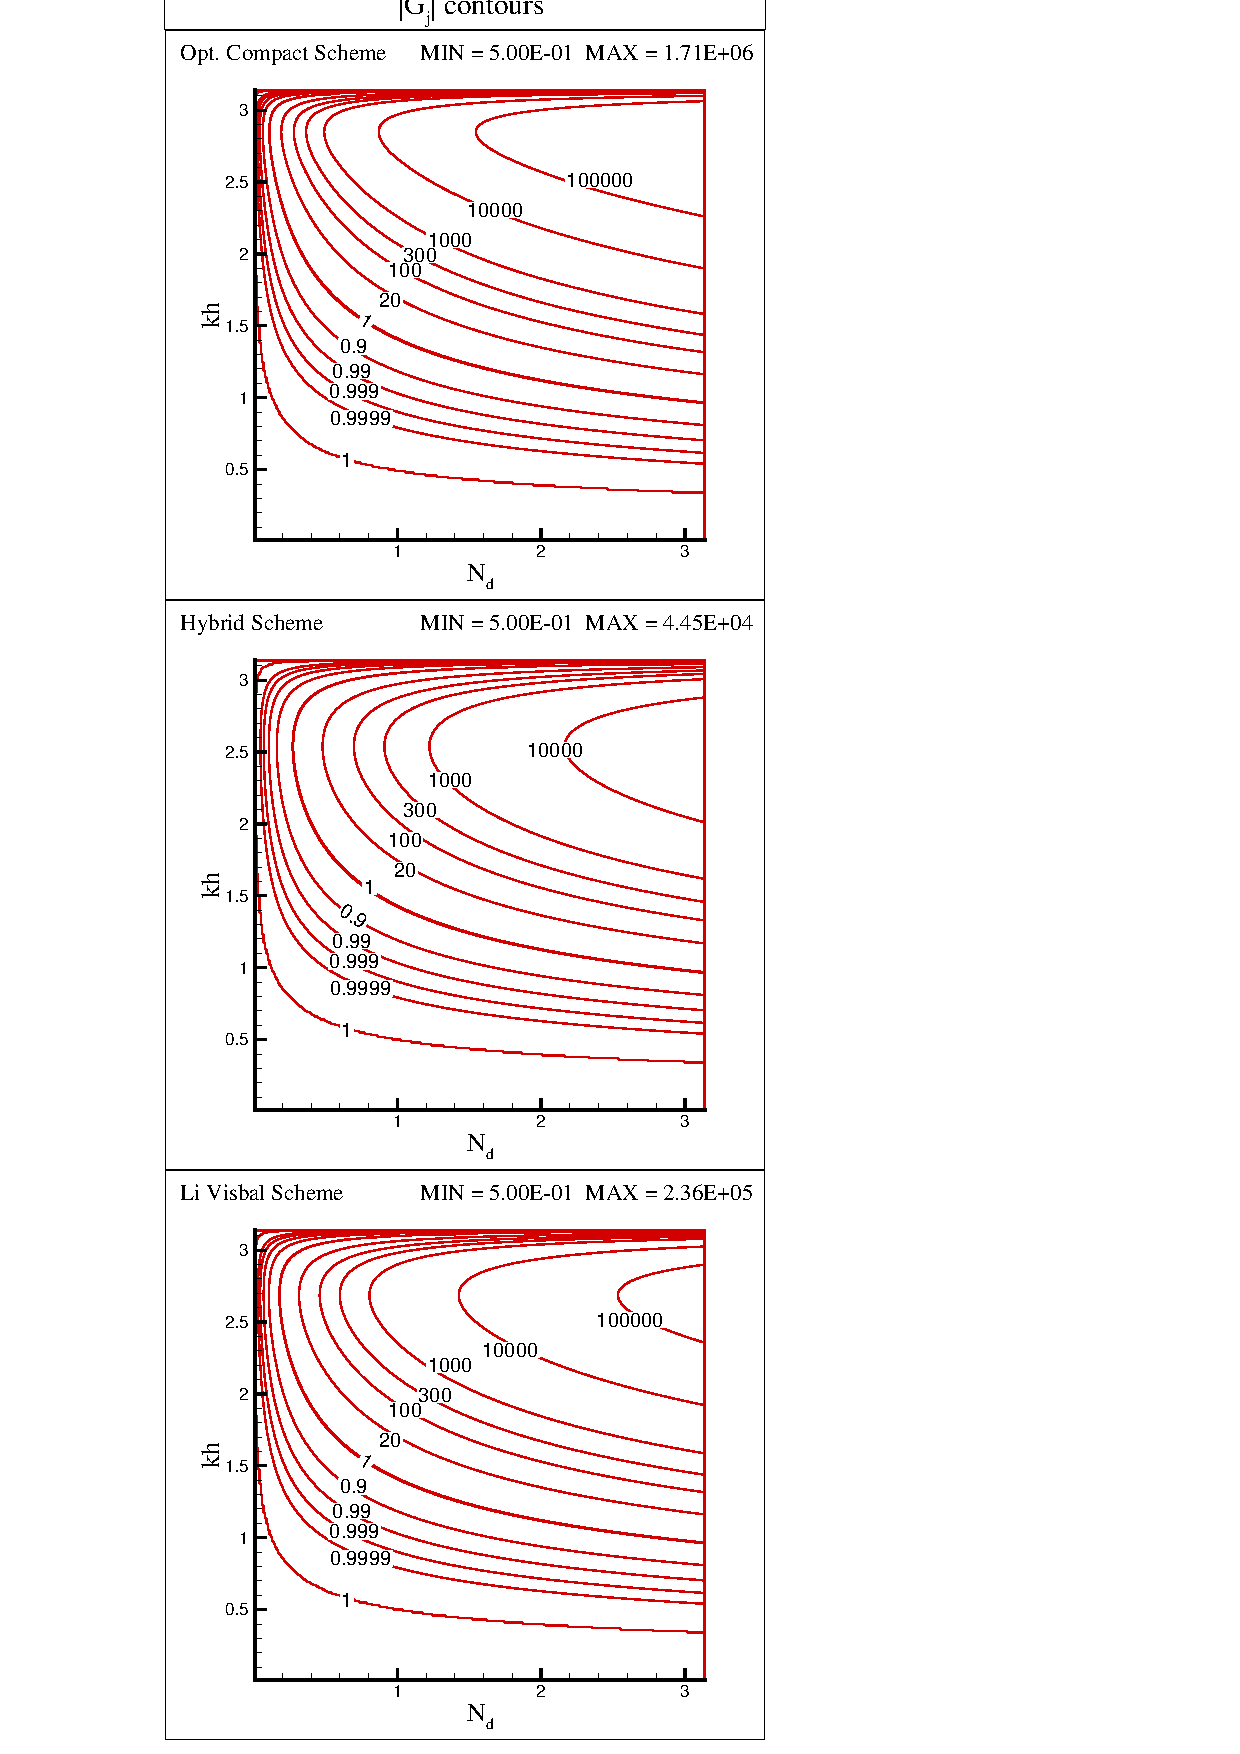
\includegraphics[scale=0.380]{Fig_7a}
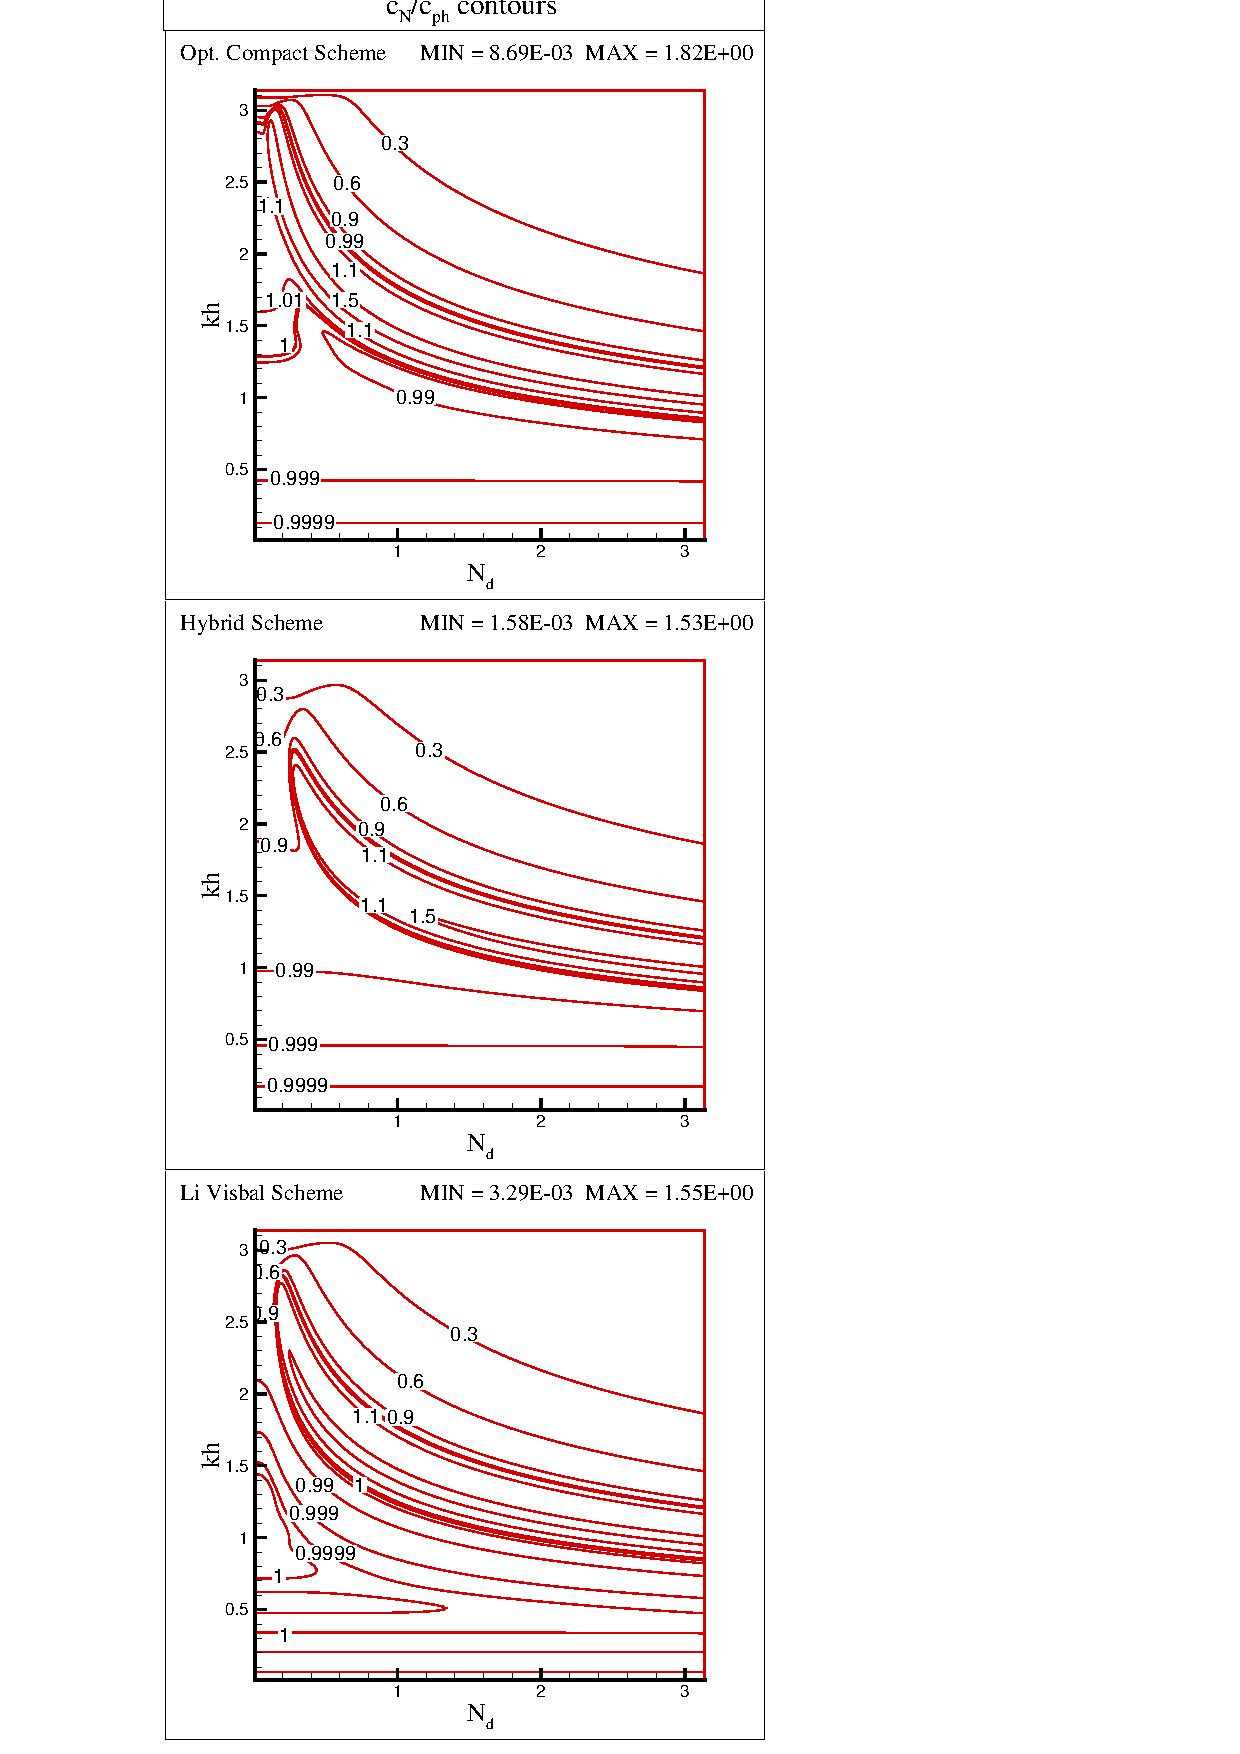
\includegraphics[scale=0.380]{Fig_7b}
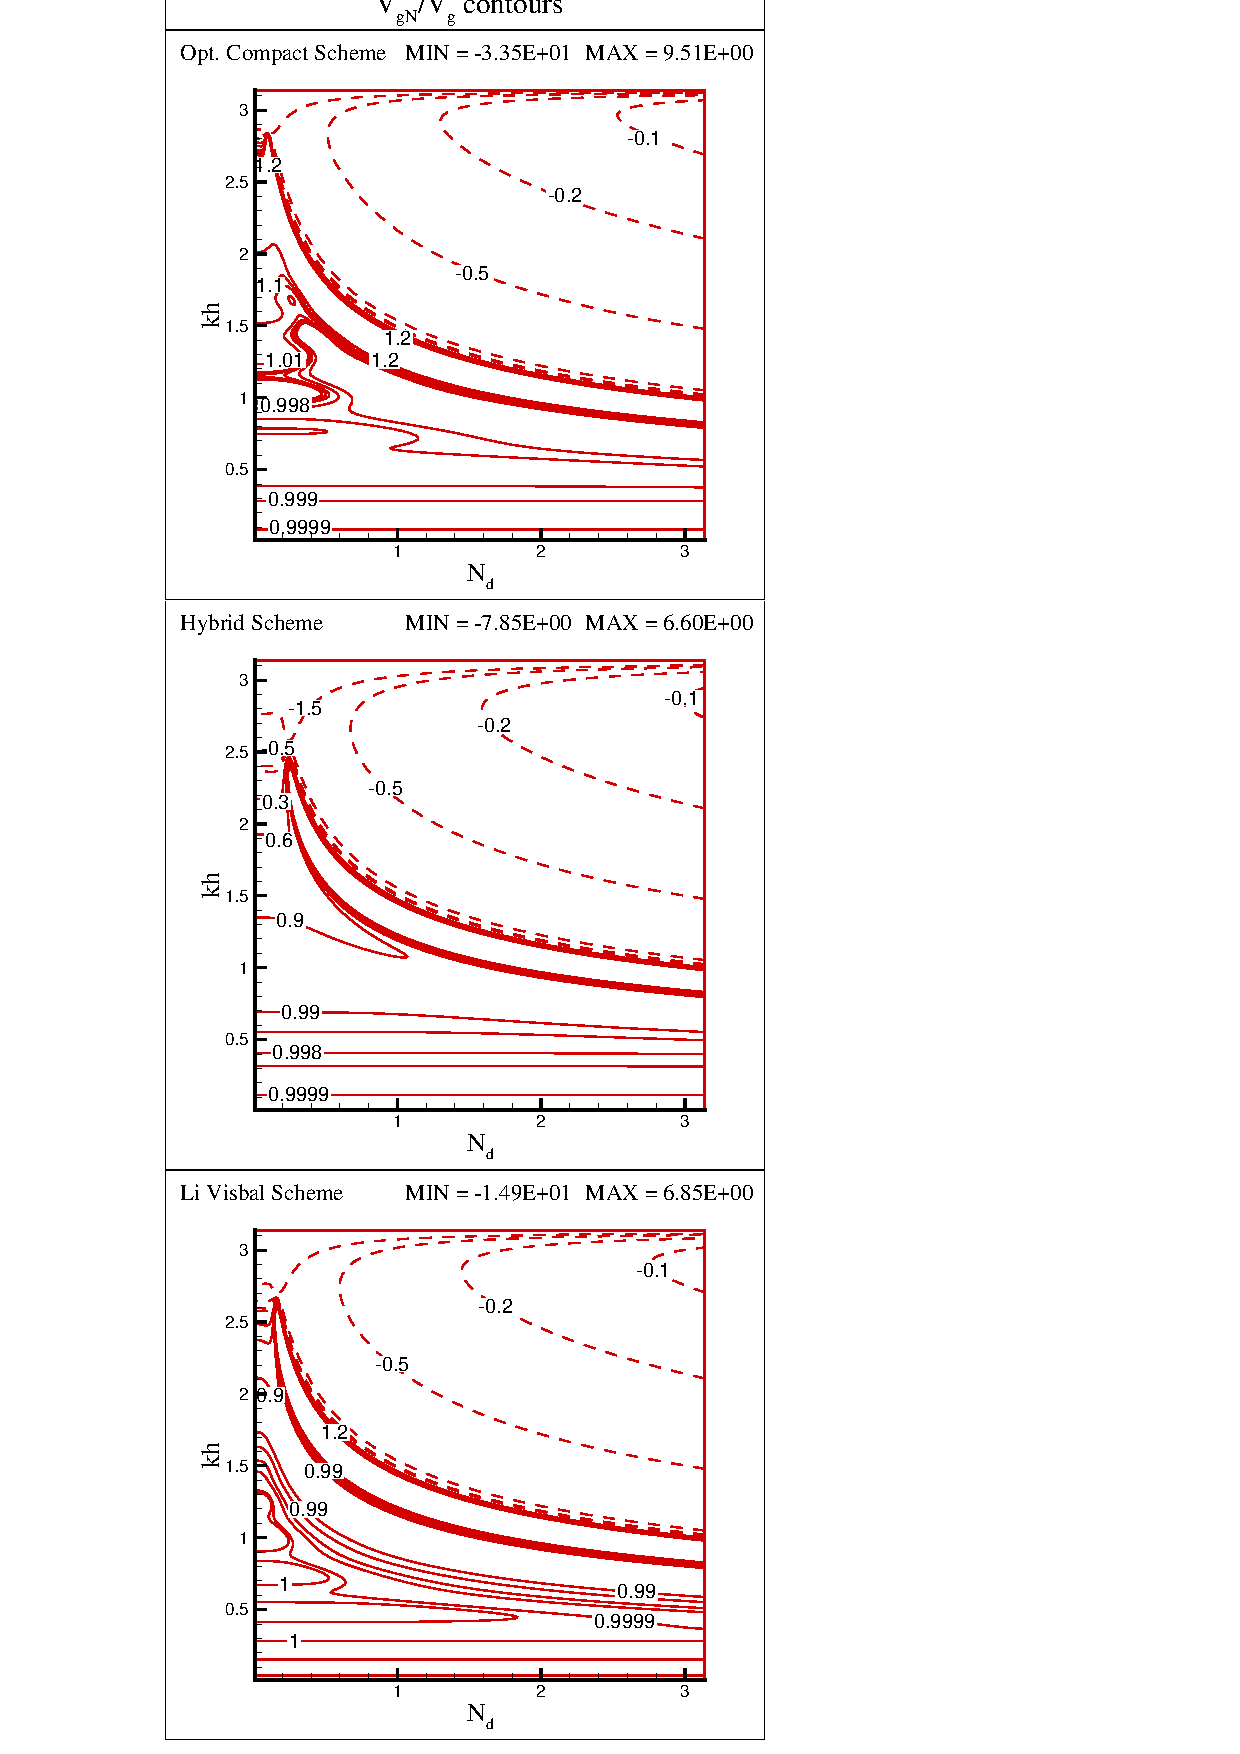
\includegraphics[scale=0.380]{Fig_7c}
\caption{Properties of various third derivative schemes plotted as a function of $N_d$ and $kh$. (i) $|G_j|$; (ii) $c_N/c_{ph}$; (iii) $V_{gN}/V_g$. }
\label{fig:props}
\end{figure}


\subsection{Simulation of One-Dimensional Dispersion Equation}
Equation \eqref{eq:disp_eqn} has been computed, using the three schemes described in section \ref{sec:num_sch}, for the following initial conditions with 
a time-step of $\Delta t =1 \times 10^{-5}$ and number of spatial nodes is $N=128$, for $-2\pi \leq x \leq 2\pi$.

Case (a): $u_0 = \sin x$; $N_d=1.056 \times 10^{-2}$; $kh=0.0981$\;\; and 

Case (b): $u_0 = \sin 8x$; $N_d=3.078 \times 10^{-4}$; $kh=0.638$



It may be noted that Case (a) involves only low wavenumber, while Case (b) involves relatively a larger wavenumber. The domain is periodic 
and the length of the domain is such that integral multiple of wavelengths are taken as the $x$-range ($-2\pi \leq x \leq 2\pi$). The exact solution 
is given by $u(x,t)=\sin[c(x+t)]$, which suggests that the wave will propagate in the negative $x$-direction with the phase speed, $-c$. 

In Figs. \ref{fig:low1} and \ref{fig:mid1}, the numerical solution and error for these two cases using optimized compact scheme have been shown. The solutions show that the major contribution to error comes from the phase and dispersion error components and the maximum occurs, where the numerical solution is given by $u_N \to 0$. This is the location where third derivative achieves its maximum value. This is in agreement with the error 
propagation equation, Eq. \eqref{eq:epe2}, which predicts the phase and dispersion errors to be maximum where the third derivatives are large.

The evolution of phase error can be represented by plotting maximum error as a function of time in Fig. \ref{fig:phase_err} for both the Cases (a) and
(b). In both the cases, Li-Visbal scheme is seen to be the most accurate of the three in simulating this model equation. However as noted before, the initial conditions for these cases involve low wavenumbers. From Fig. \ref{fig:props}, it is evident that Li-Visbal scheme has a DRP region which is 
very good up to $kh \leq 0.7$, for small values of $N_d$. Interestingly, for Case (a) with initial condition given by $u_0 = \sin x$, the hybrid scheme performs slightly better than optimized compact scheme, which can be noted if one zooms in Fig. \ref{fig:keq} for very low values of $kh$. The converse 
is true for Case (b) with the initial condition $u_0 = \sin 8x$, which involves relatively larger value of $kh$, for which the optimized compact scheme 
is superior over the hybrid scheme. For the chosen grid spacing for Case (b), one can note the properties for the relevant value of $kh=0.638$. From 
Fig. \ref{fig:props}, the optimized compact scheme has lesser phase error given by $c_N/c_{ph} \approx 0.999$, as compared to the hybrid scheme which 
has $c_N/c_{ph} \approx 0.99$.

The error analysis of linear dispersion equation suggests that all the three schemes give reasonably accurate solutions only with $N_d \leq 0.1$ and $kh \leq 0.5$. While this exercise may seemingly show superiority of solving linear dispersion equation \eqref{eq:disp_eqn} by Li-Visbal scheme over the other two schemes, we again emphasize that solving a nonlinear equation, the outcome will be determined once again, from the properties in Fig. \ref{fig:props} and the conclusions would be distinctly different. This is shown next. 

%-----------------------------------------------------------------------------------------------------
\begin{figure}[!h]
\center
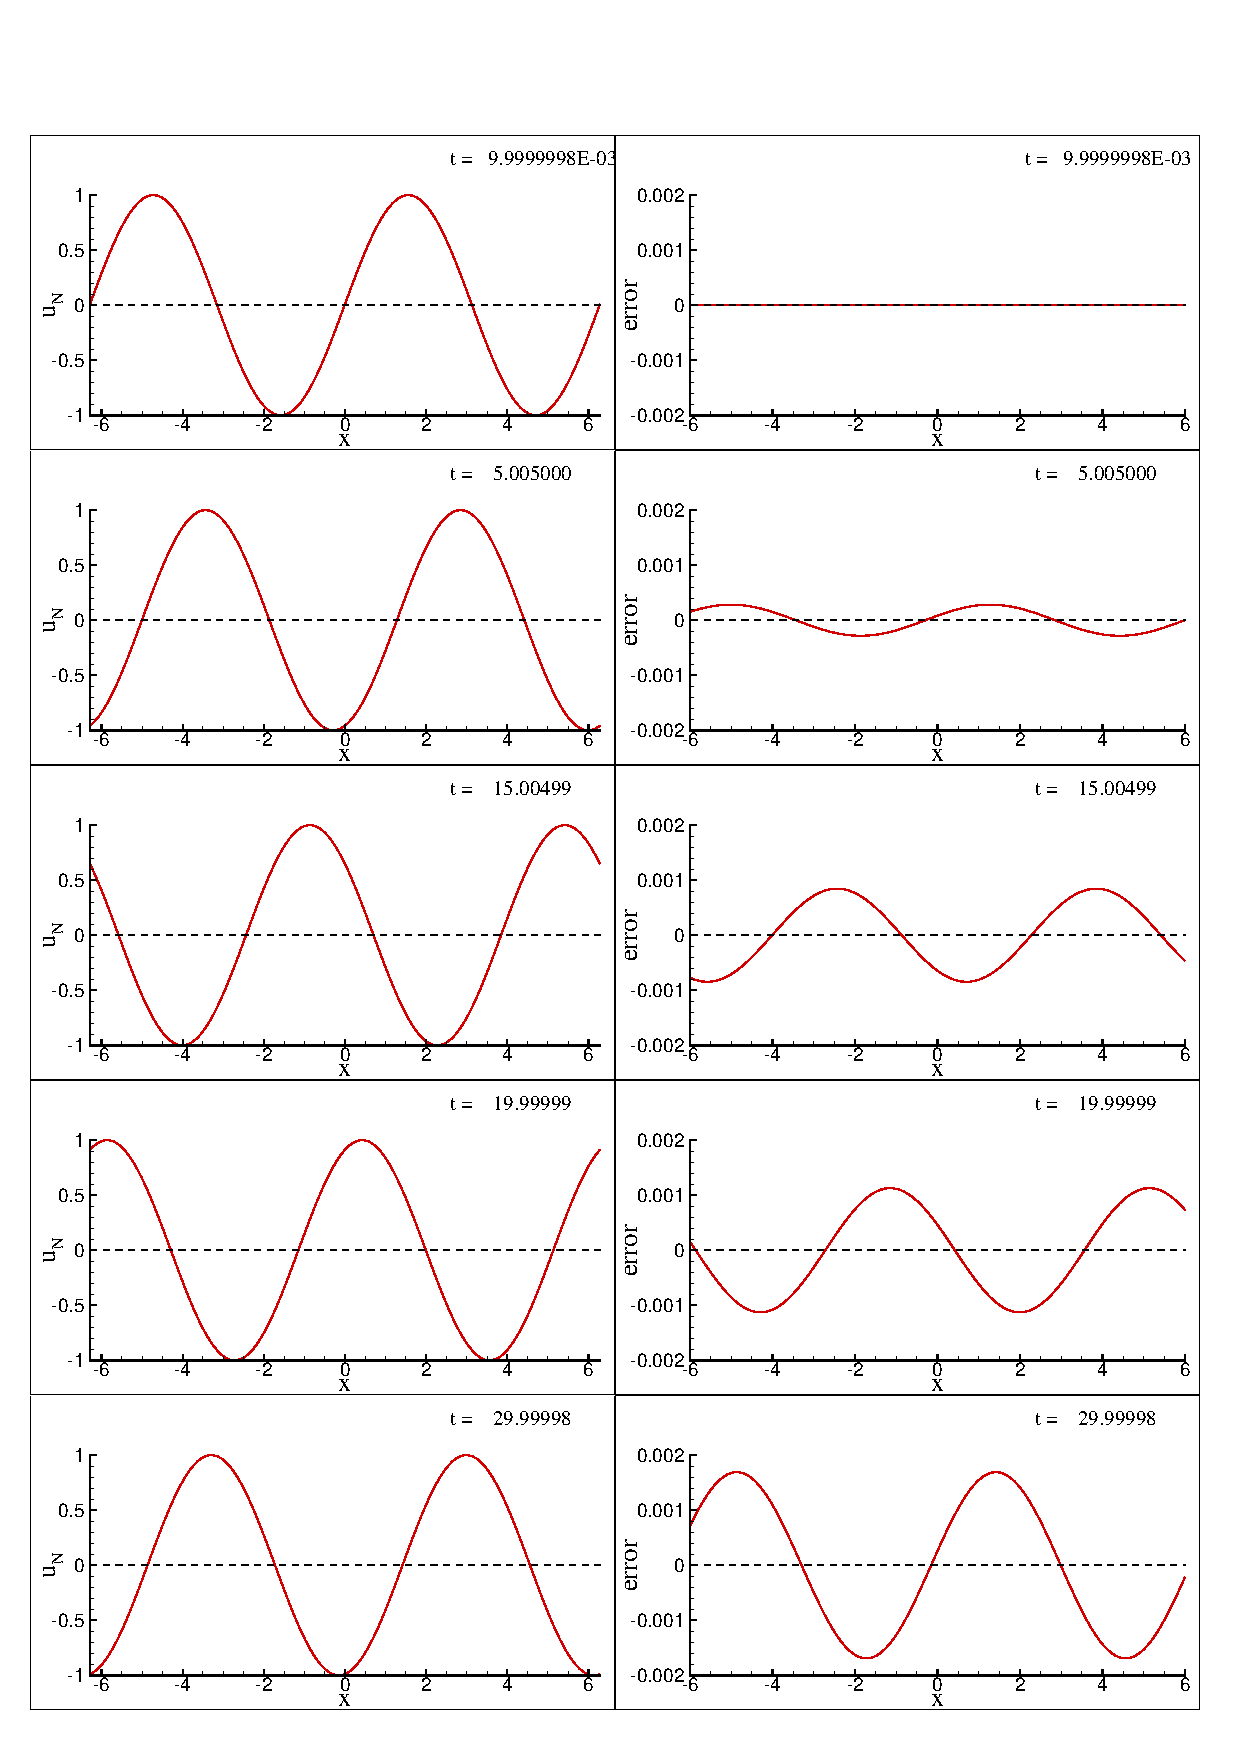
\includegraphics[width=0.8\linewidth]{Fig_8}
\caption{Evolution of numerical solution and error for $u_0=\sin x$ solved using optimized compact scheme.}
\label{fig:low1}
\end{figure}

\begin{figure}[!h]
\center
\includegraphics[width=0.8\linewidth]{Fig_9}
\caption{Evolution of numerical solution and error for $u_0=\sin 8x$ solved using optimized compact scheme.}
\label{fig:mid1}
\end{figure}

%-----------------------------------------------------------------------------------------------------
\begin{figure}
\center
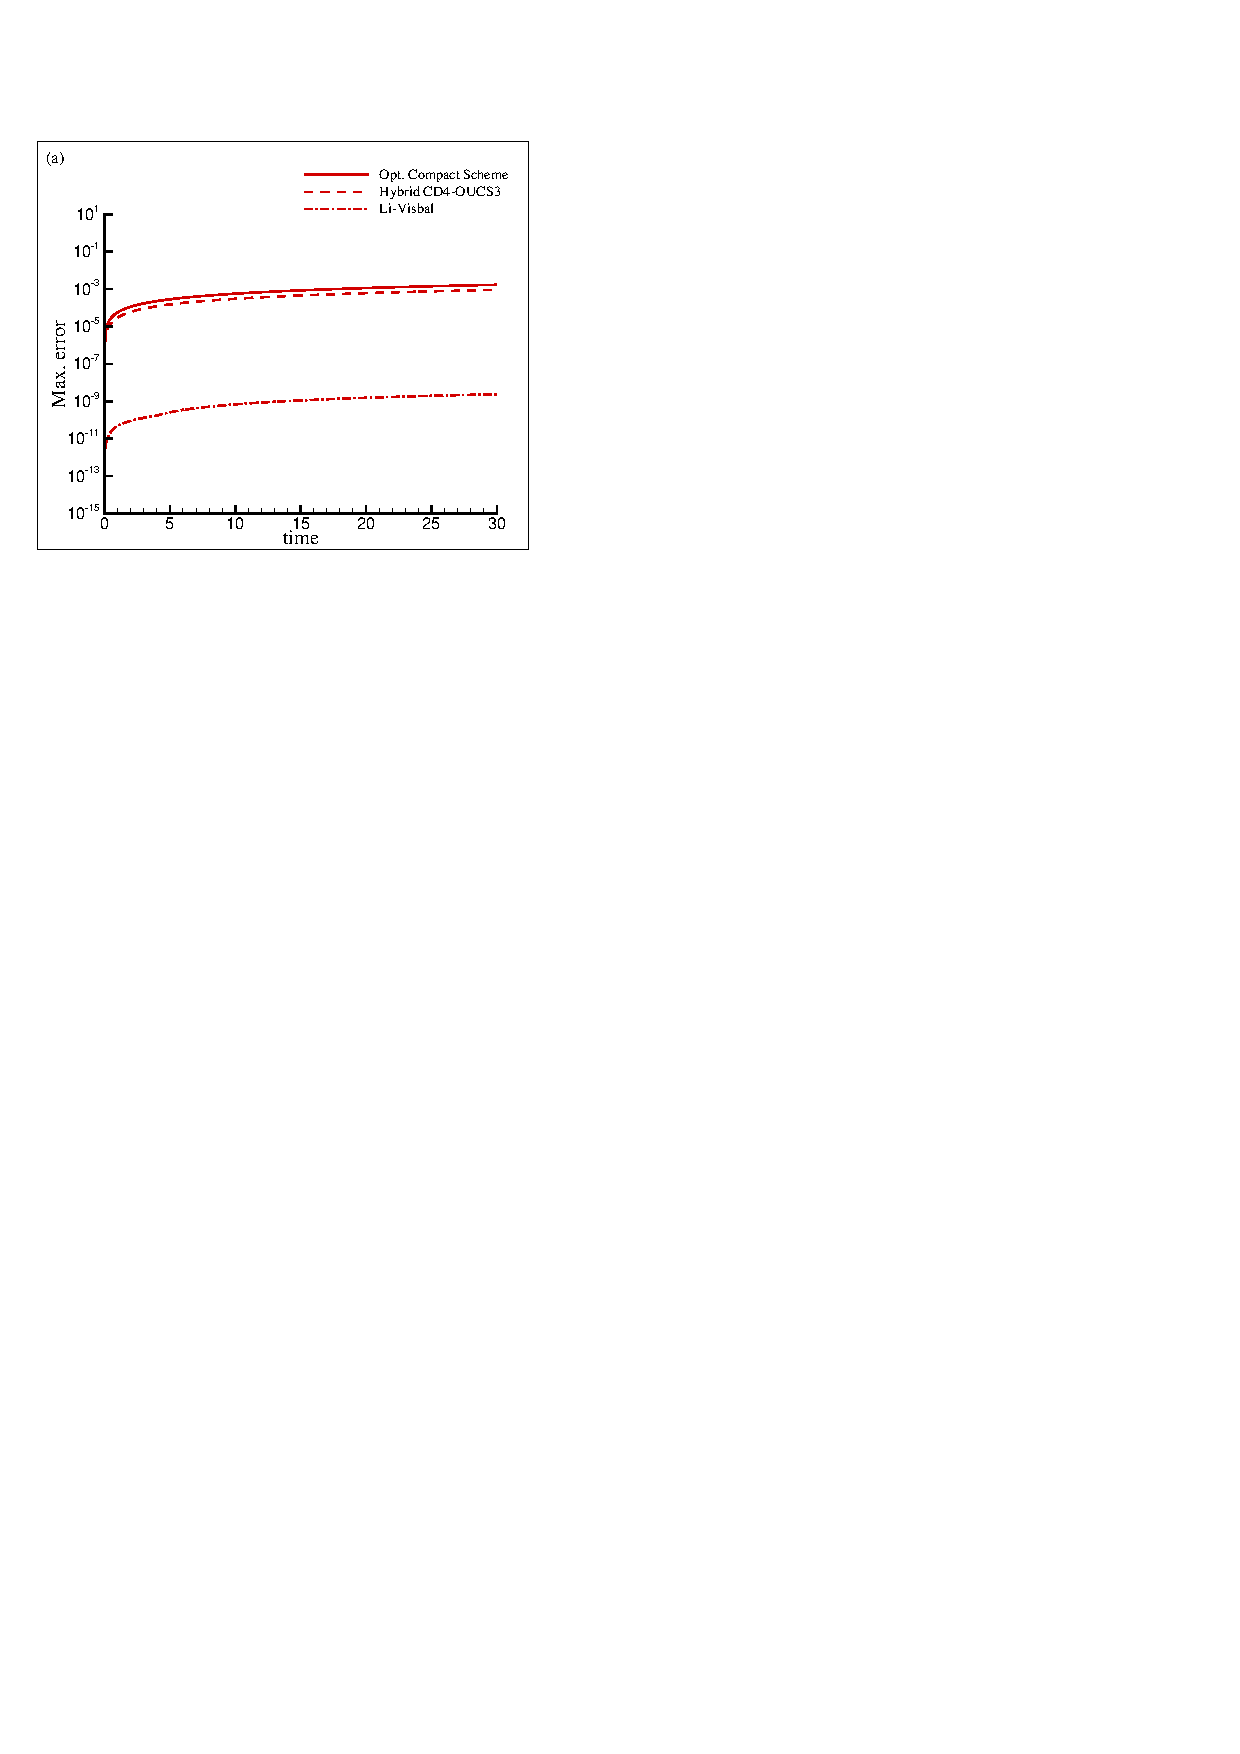
\includegraphics[width=0.48\linewidth]{Fig_10a}
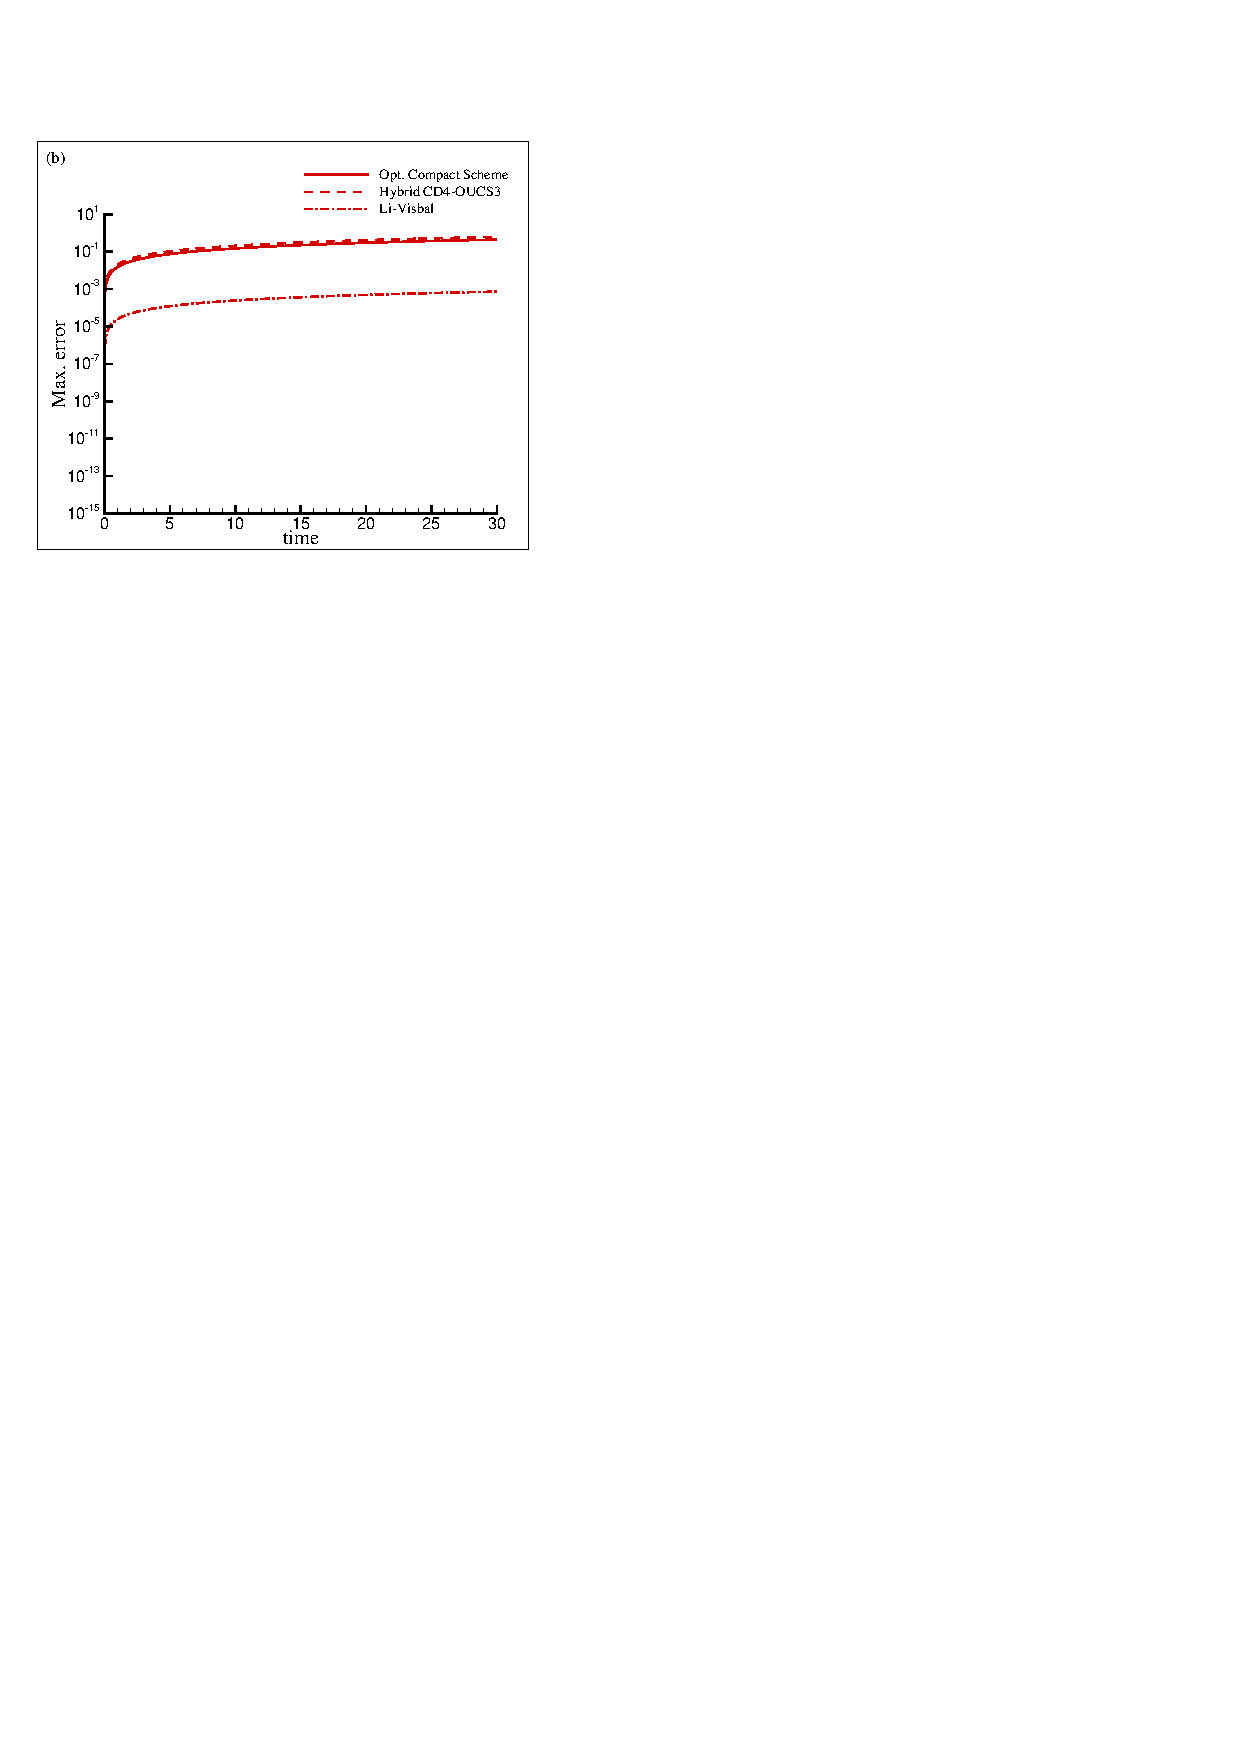
\includegraphics[width=0.48\linewidth]{Fig_10b}
\caption{Evolution of maximum error with time while solving one-dimensional dispersion equation with initial condition (a) $u_0=\sin x$ ; (b) $u_0=\sin 8x$, for various schemes.}
\label{fig:phase_err}
\end{figure}

%---------------------------------------------------------------------------------------------------
\section{Results and Discussion}
\label{sec:res}
The utility of the two schemes developed here is demonstrated by solving the KdV equation. A periodic computational domain, $-50\leq x \leq 50$ is 
considered for both one- and two-soliton cases. To examine the dependence of the numerical solution on grid spacing and time-step, simulations are performed with the following number of nodes ($N$) and time-steps ($\Delta t$)
\begin{itemize}
  \item $N=1024$ and $\Delta t = 1 \times 10^{-5}$
  \item $N=2048$ and $\Delta t = 1 \times 10^{-5}$
  \item $N=2048$ and $\Delta t = 1 \times 10^{-6}$
\end{itemize}
The error incurred is defined as before by $|u - u_N|$, with $u_N$ as the computed solution. For this study, the results of simulation using the optimized compact scheme described in subsection \ref{subsec:OCS}, have been presented here.
For the one-soliton case the absolute error is studied, at three different time instants in Fig. \ref{fig:one1} with reference to soliton locations shown in Fig. \ref{fig:one0}.
Using more number of nodes to discretize the domain, i.e., with $N=2048$, resulted in considerable reduction of error, as noted by comparing the 
solutions in frames (a) and (b) of Fig. \ref{fig:one1}.  Doubling the number of points in Fig. 
\ref{fig:one1}(b) as compared to Fig. \ref{fig:one1}(a), the average error comes down by almost an order of magnitude. The maximum error occurs
near the vicinity of the soliton due to the phase error, with the computed solution moving slower compared to the exact solution, i.e., $c_N < c$. 

%-----------------------------------------------------------------------------------------------------
\begin{figure}
\centerline{
\includegraphics[width=0.5\linewidth]{Fig_11}
}
\caption{Representative numerical solution for one-soliton case, showing the location of the soliton at three time instants}
\label{fig:one0}
\end{figure}

\begin{figure}[h!]
\centerline{
\subfloat[]{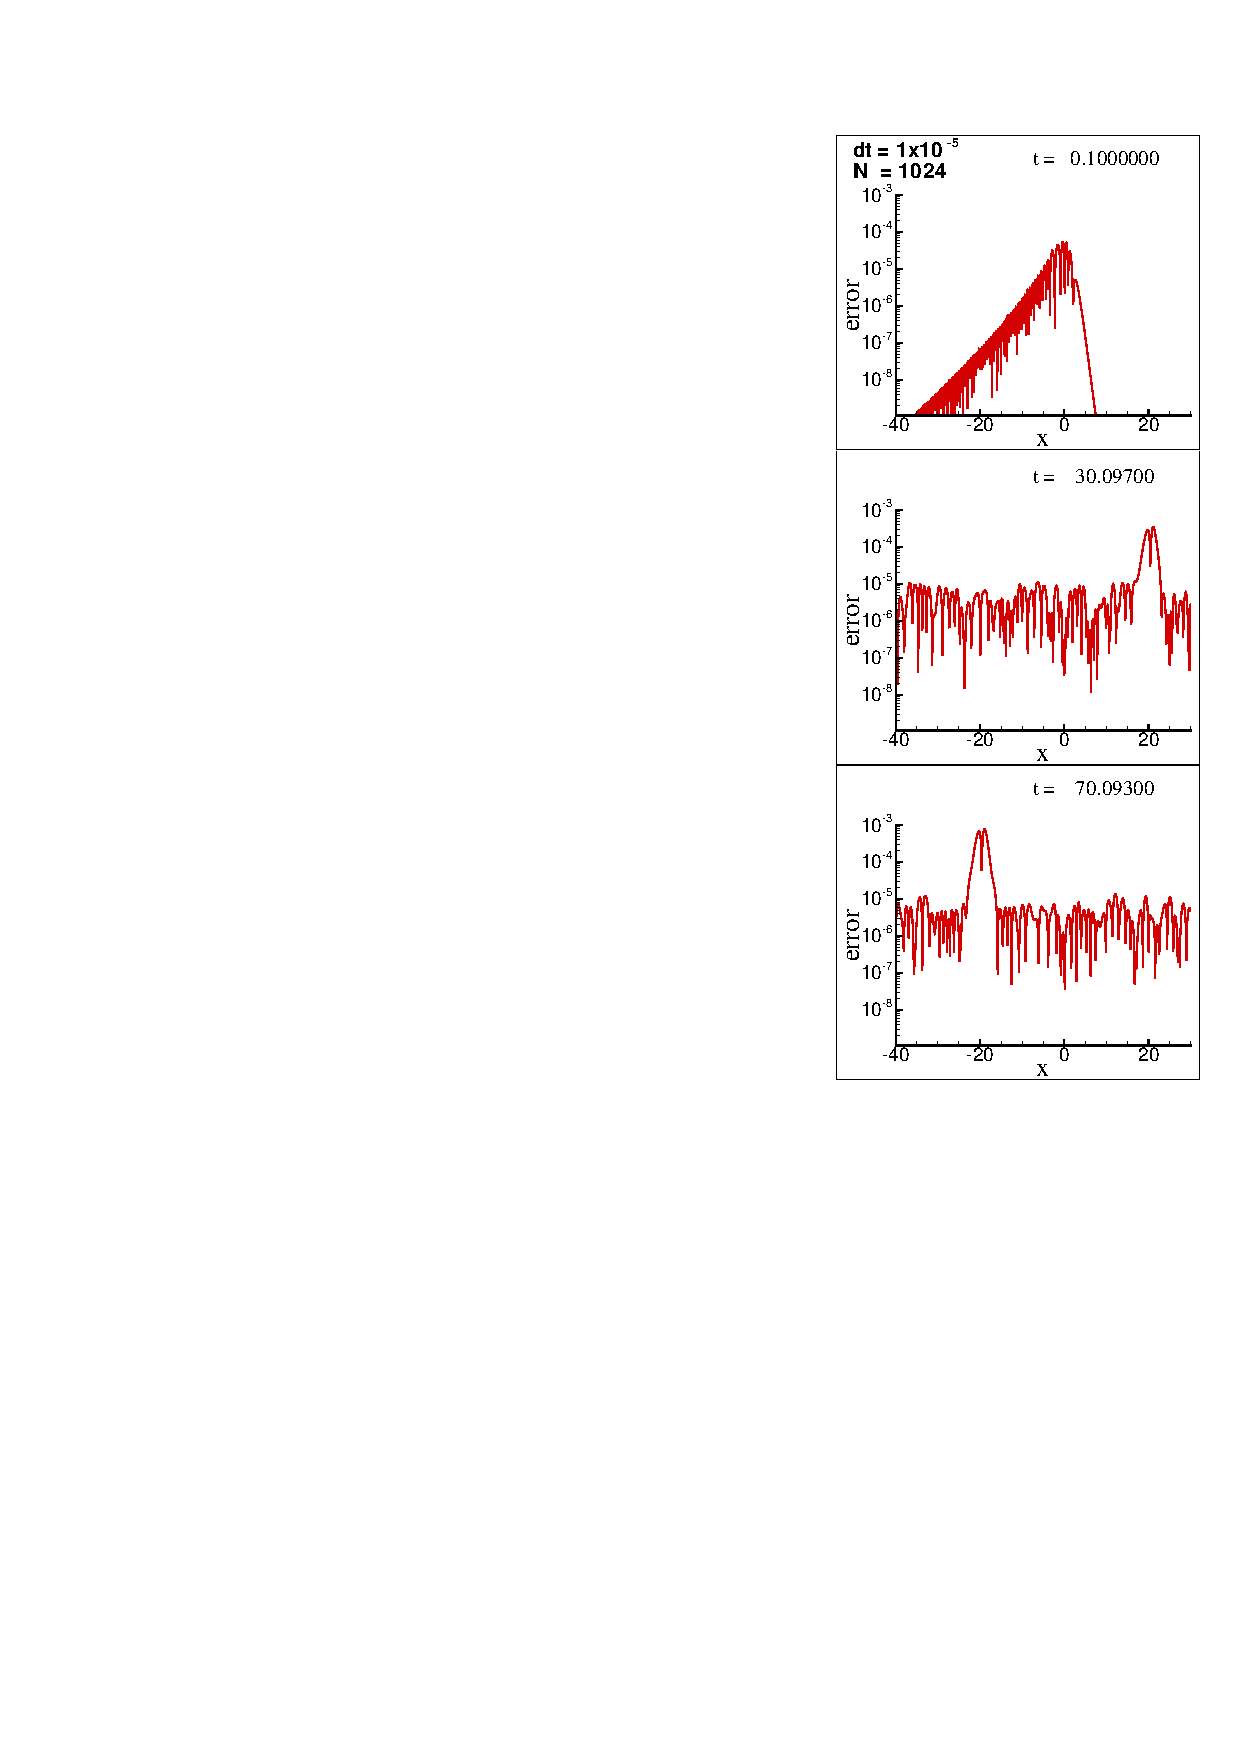
\includegraphics[width=0.33\linewidth]{Fig_12a}}
\subfloat[]{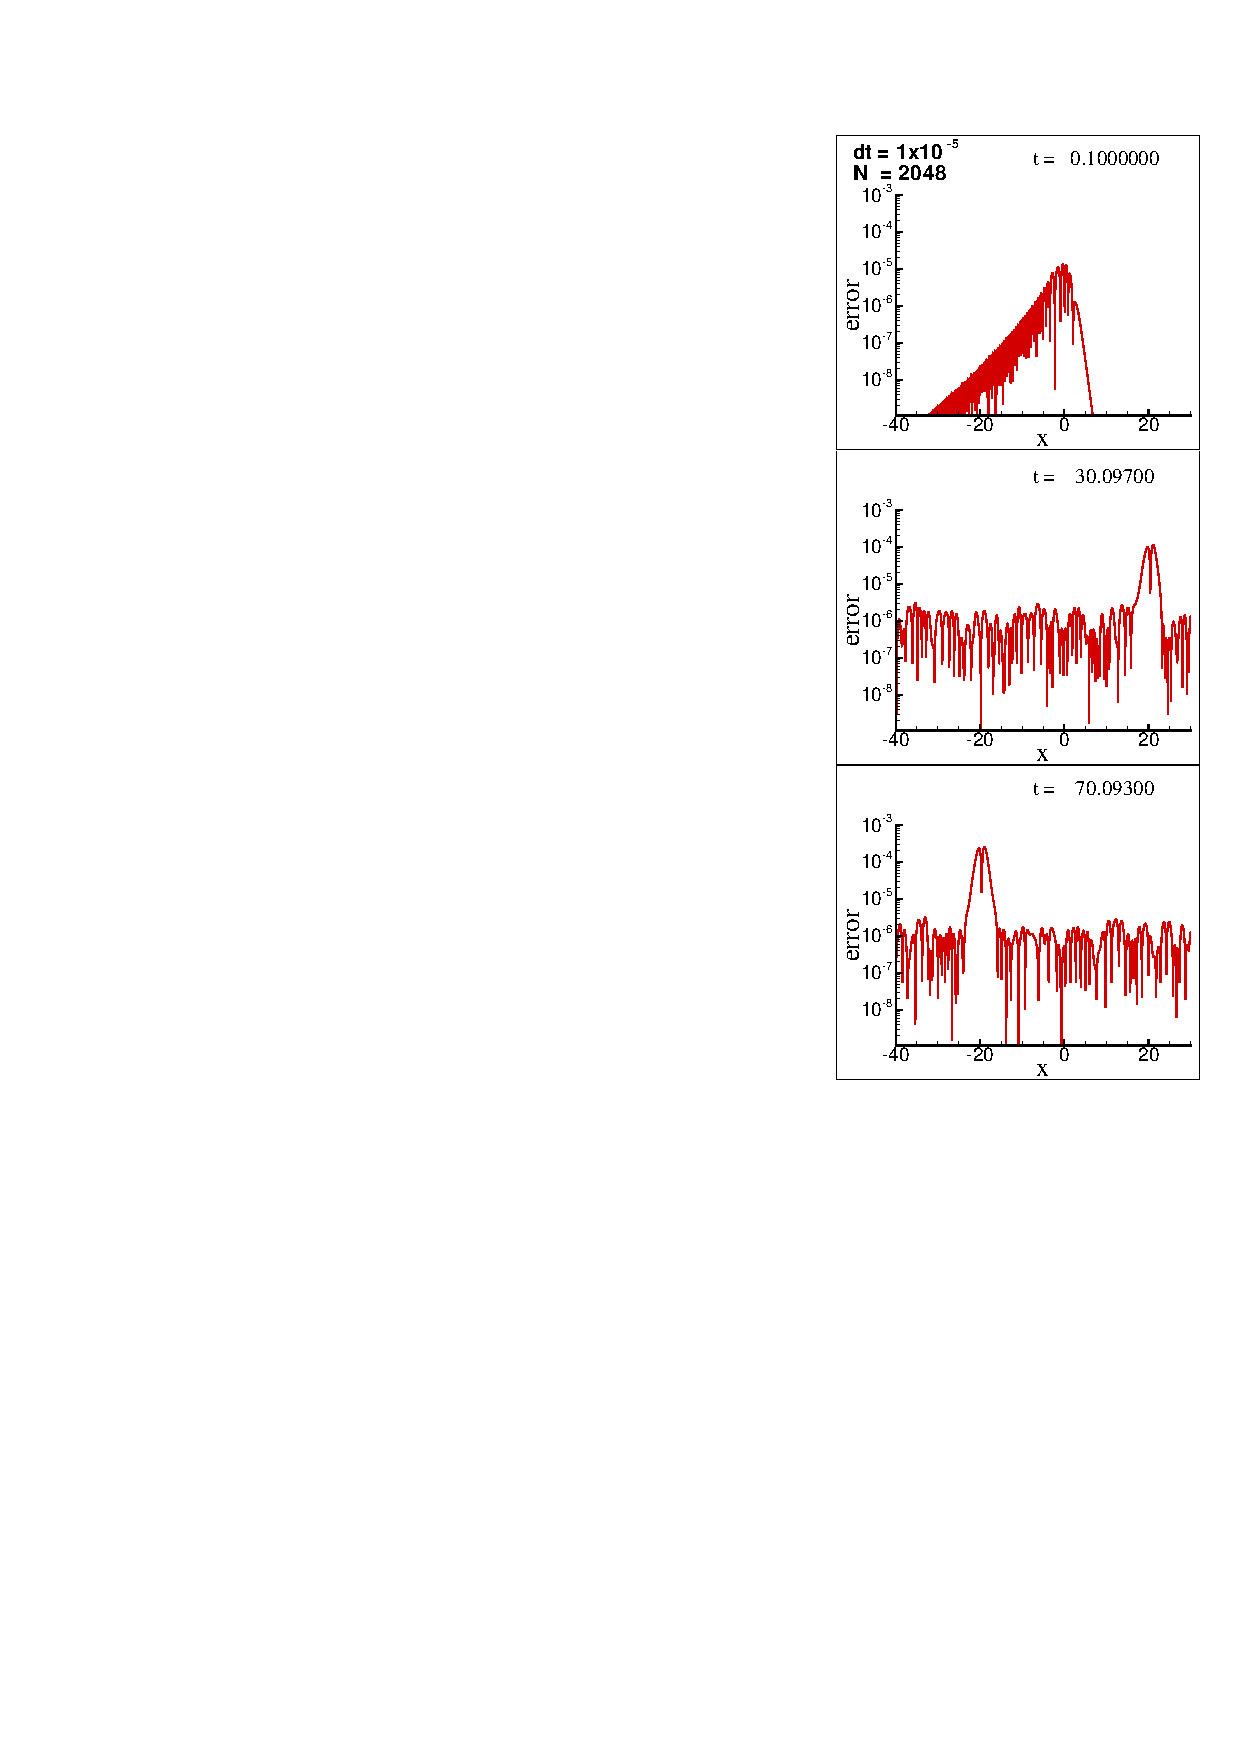
\includegraphics[width=0.33\linewidth]{Fig_12b}}
\subfloat[]{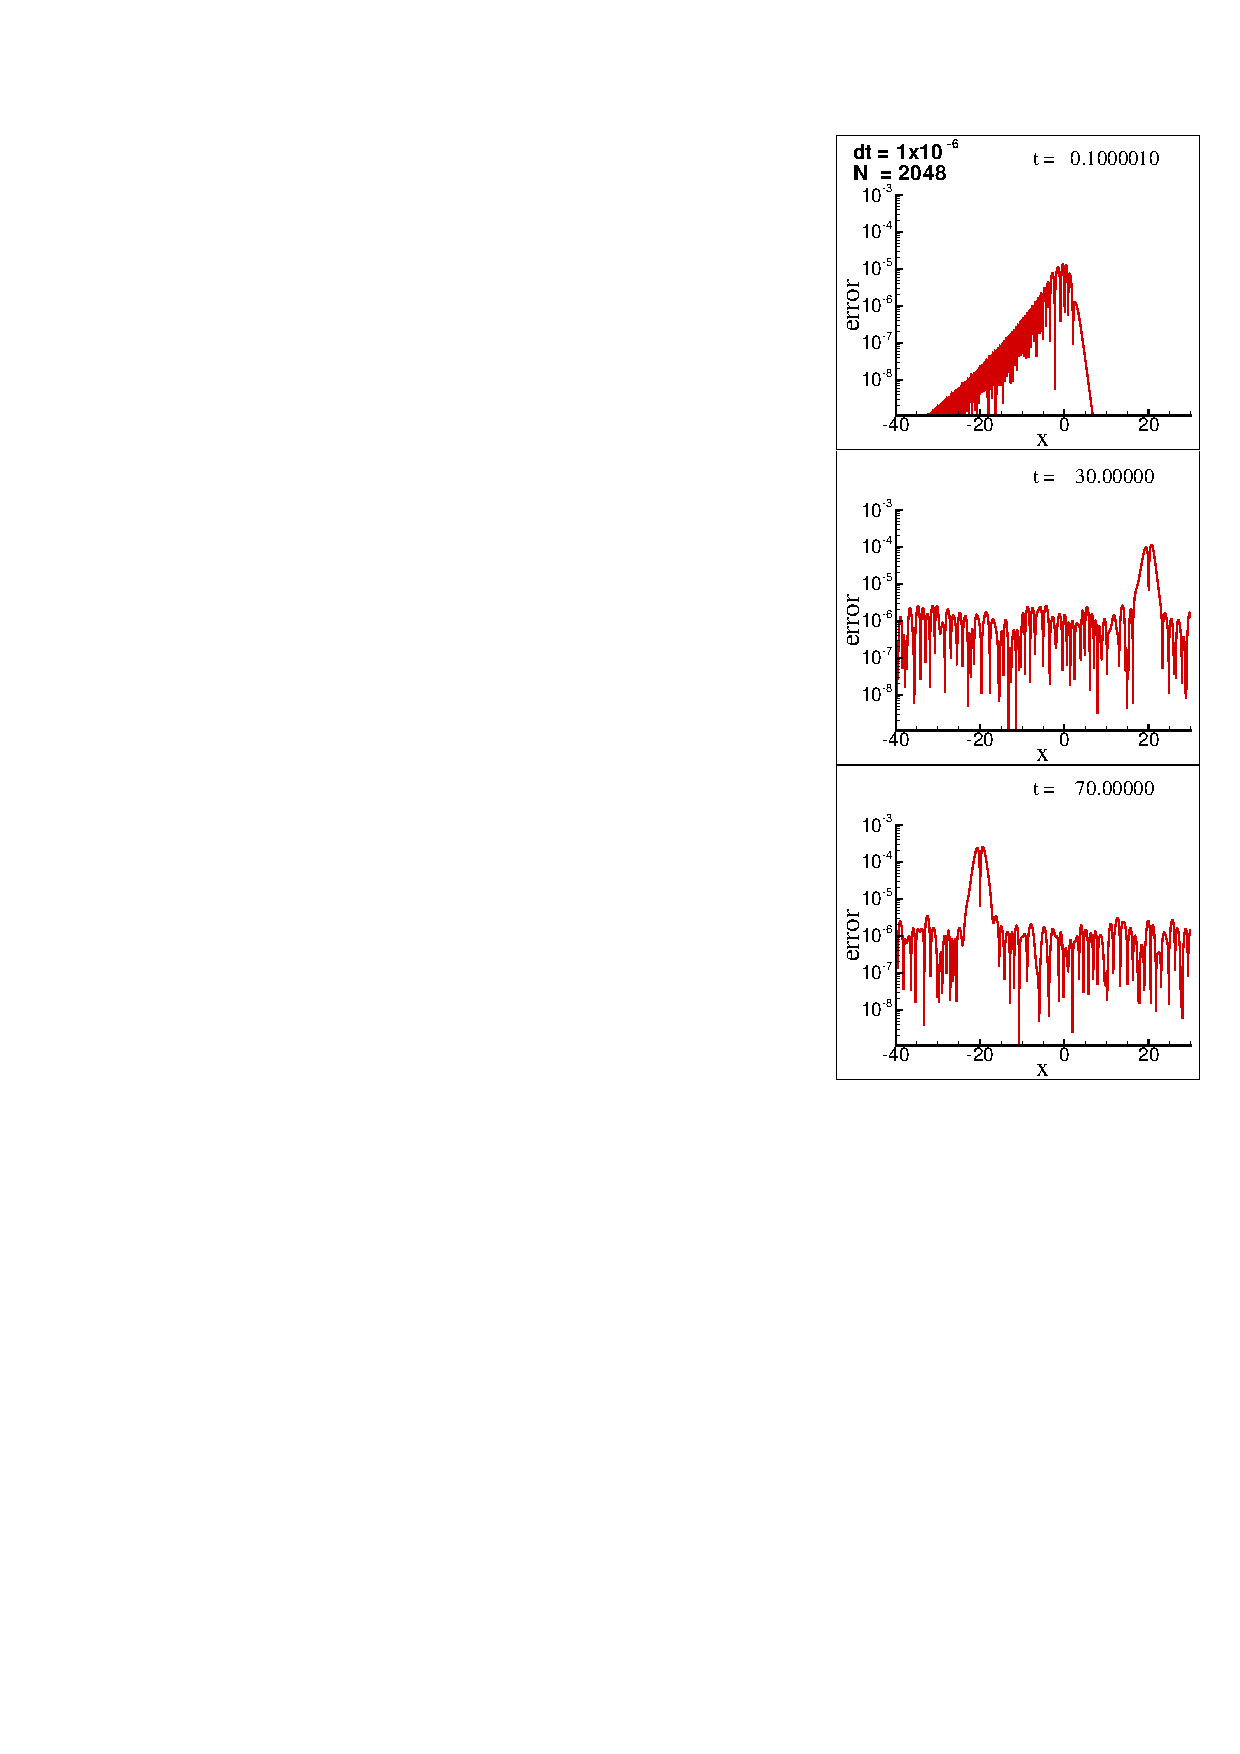
\includegraphics[width=0.33\linewidth]{Fig_12c}}
}
\caption{Evolution of error for one-soliton case showing the effect of grid spacing and time-step with respect to optimized compact scheme}
\label{fig:one1}
\end{figure}


\begin{figure}[h!]
\centerline{
\subfloat[]{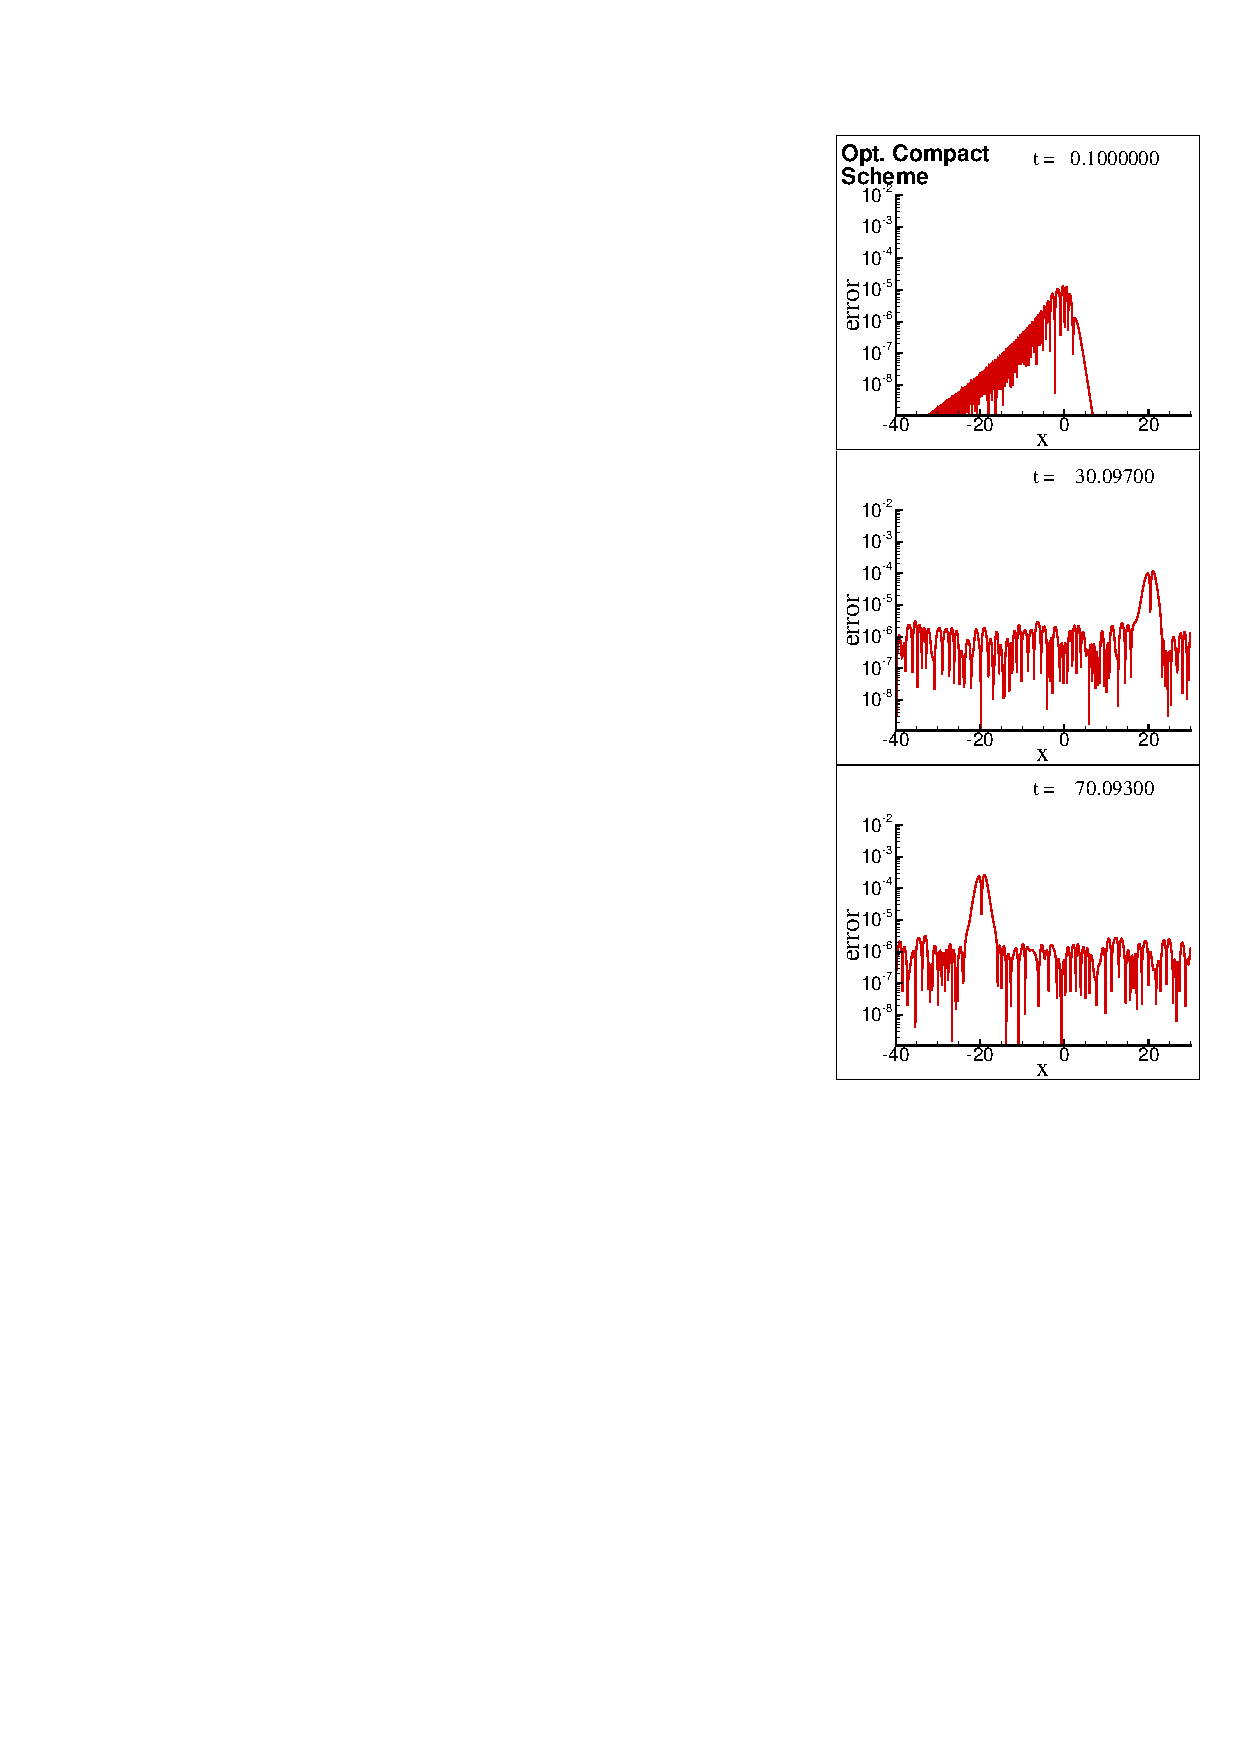
\includegraphics[width=0.33\linewidth]{Fig_13a}}
\subfloat[]{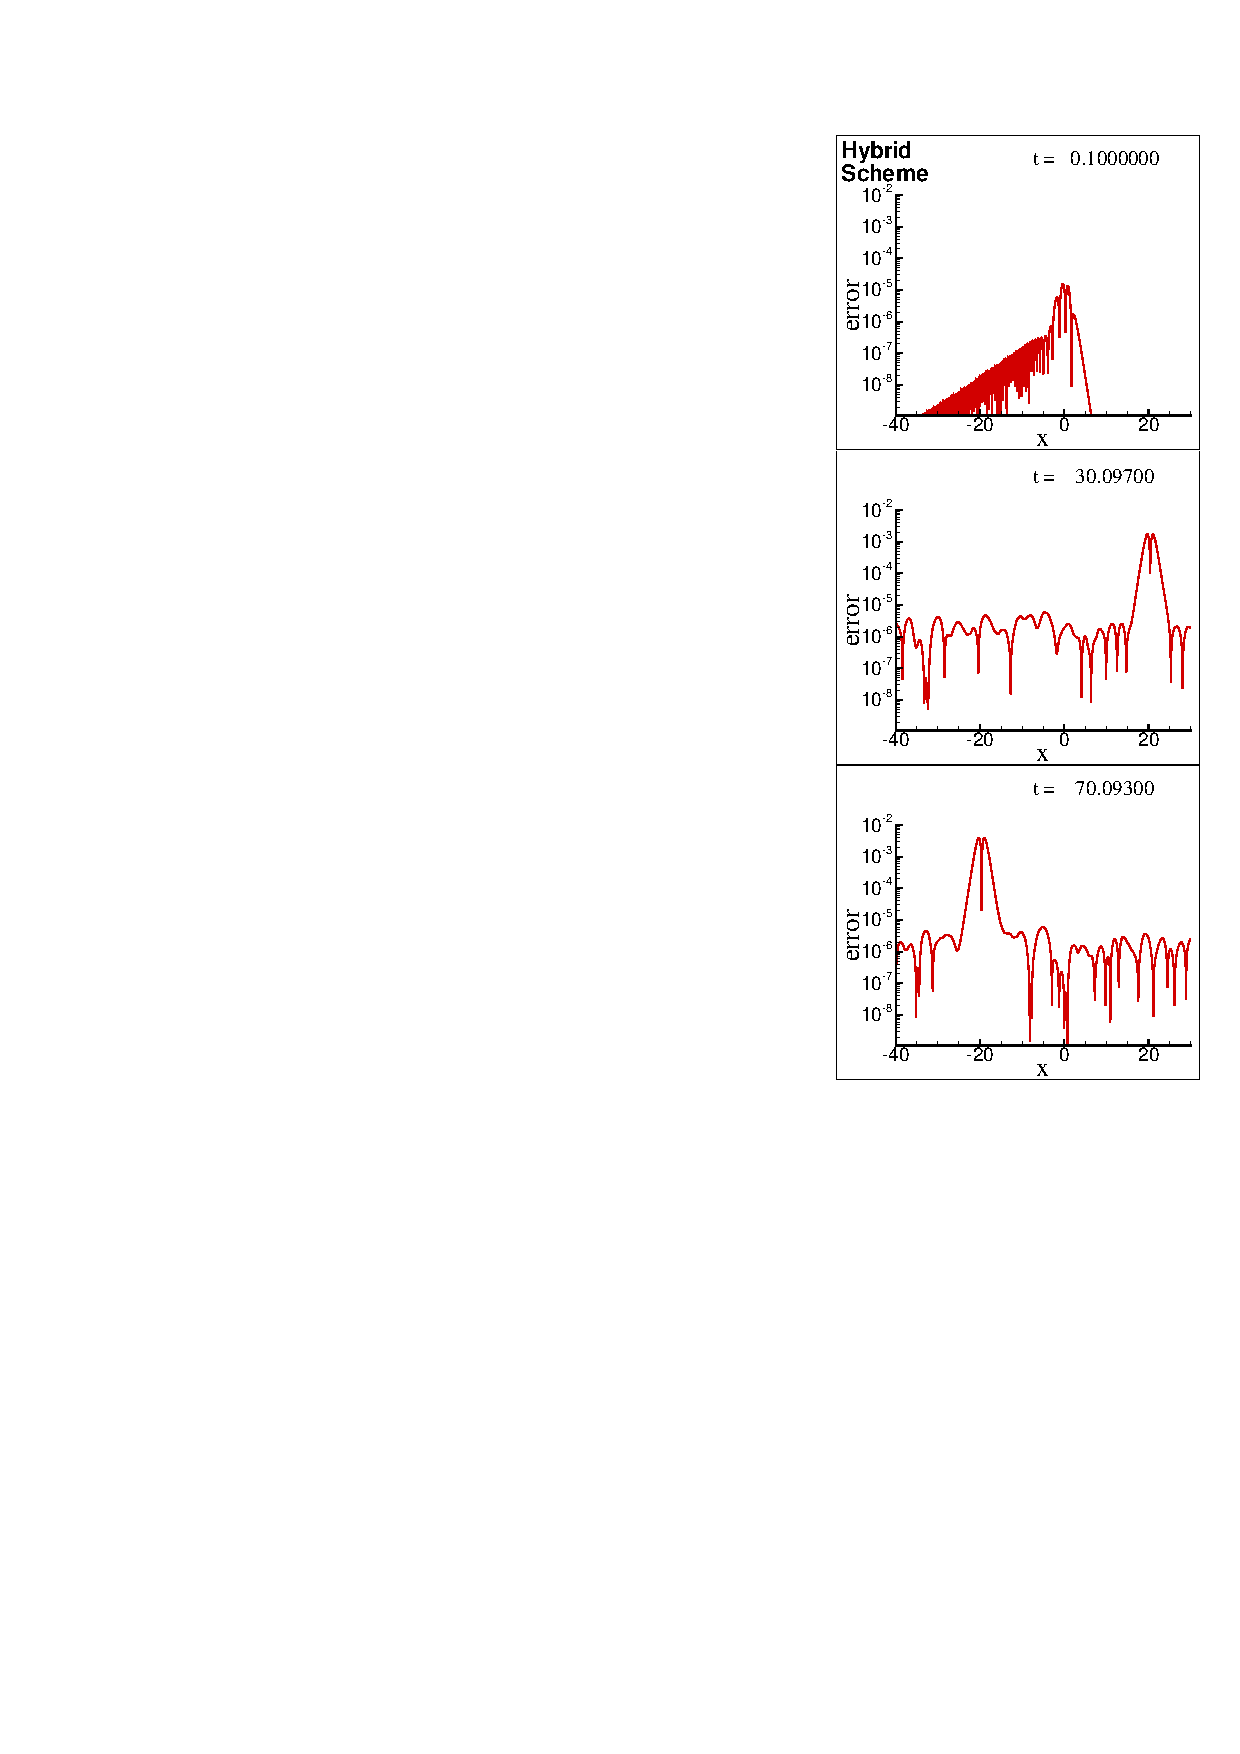
\includegraphics[width=0.33\linewidth]{Fig_13b}}
\subfloat[]{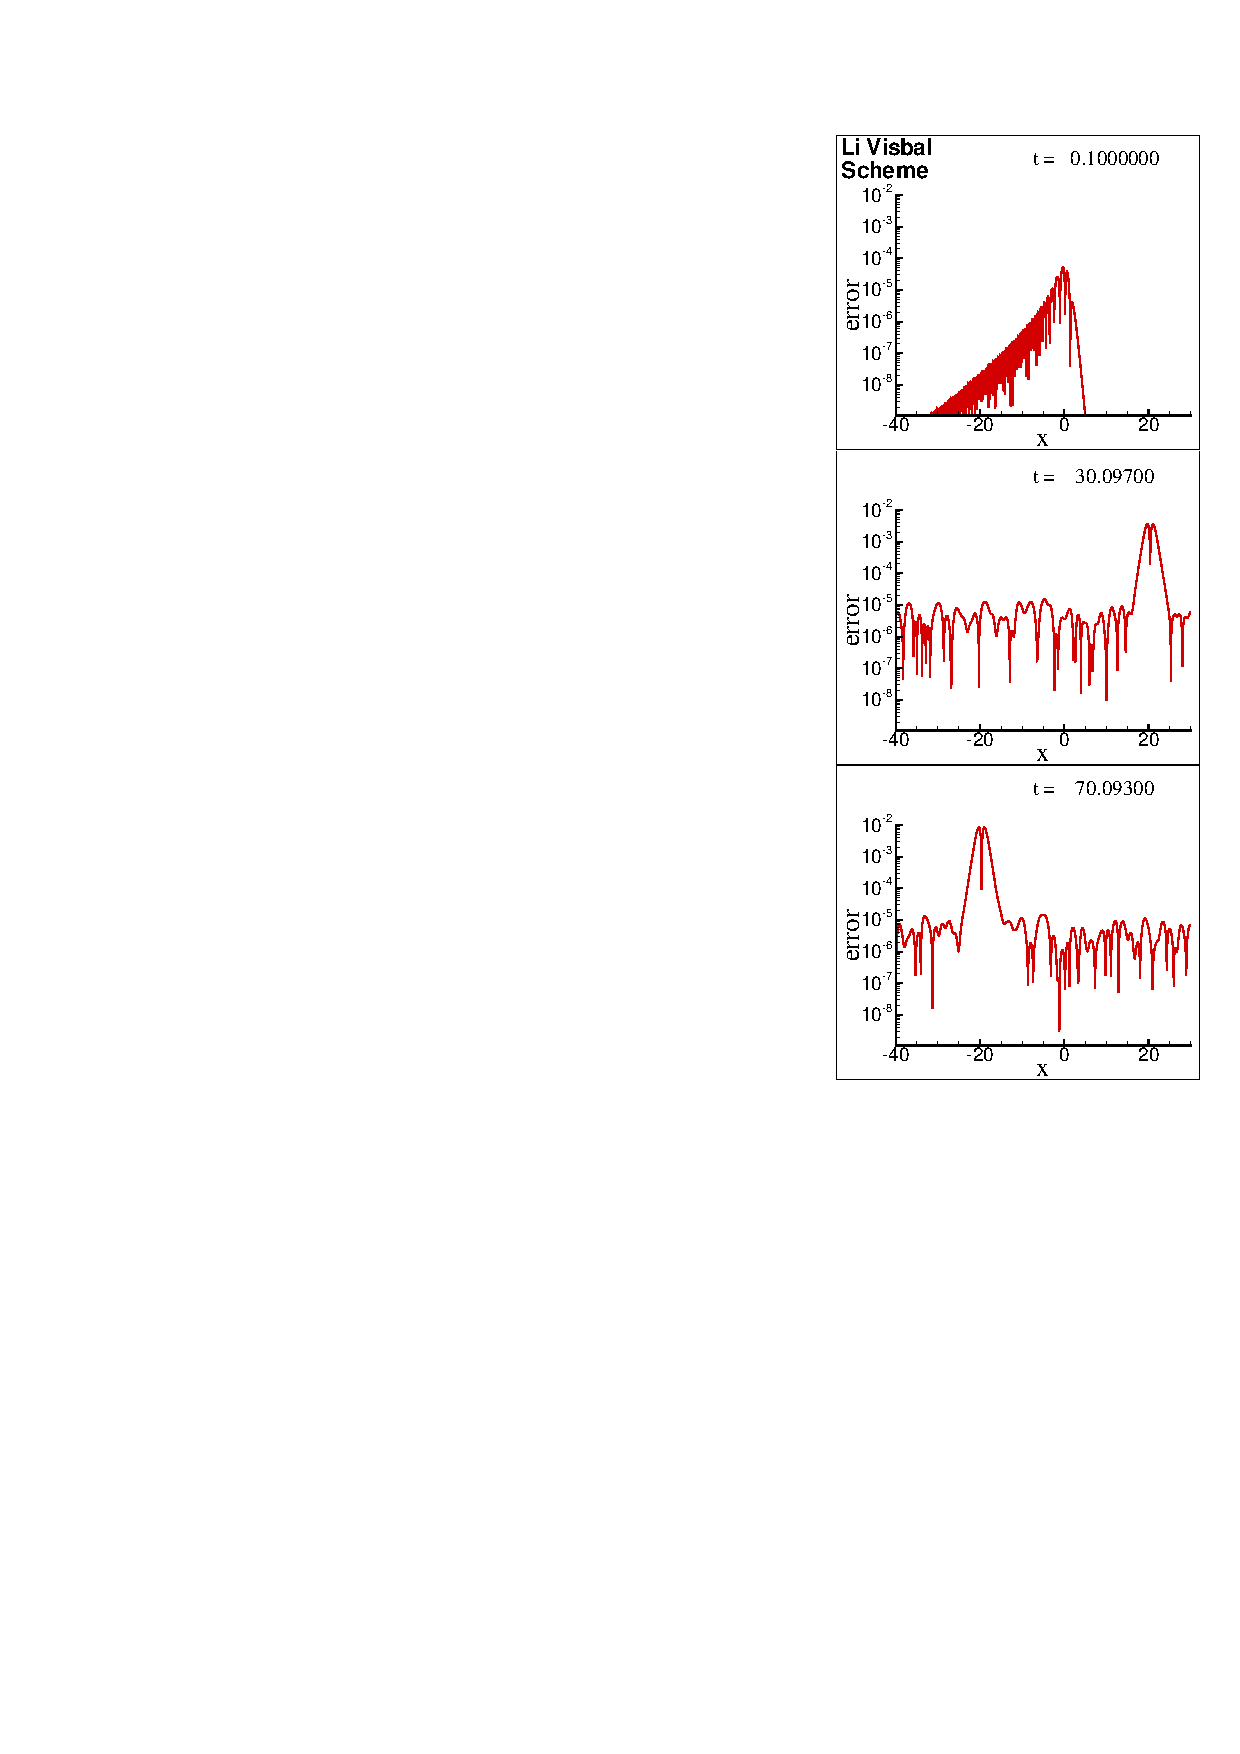
\includegraphics[width=0.33\linewidth]{Fig_13c}}
}
\caption{Evolution of error for one-soliton case comparing different methods}
\label{fig:one2}
\end{figure}

%-----------------------------------------------------------------------------------------------------
\begin{figure}[h!]
\center
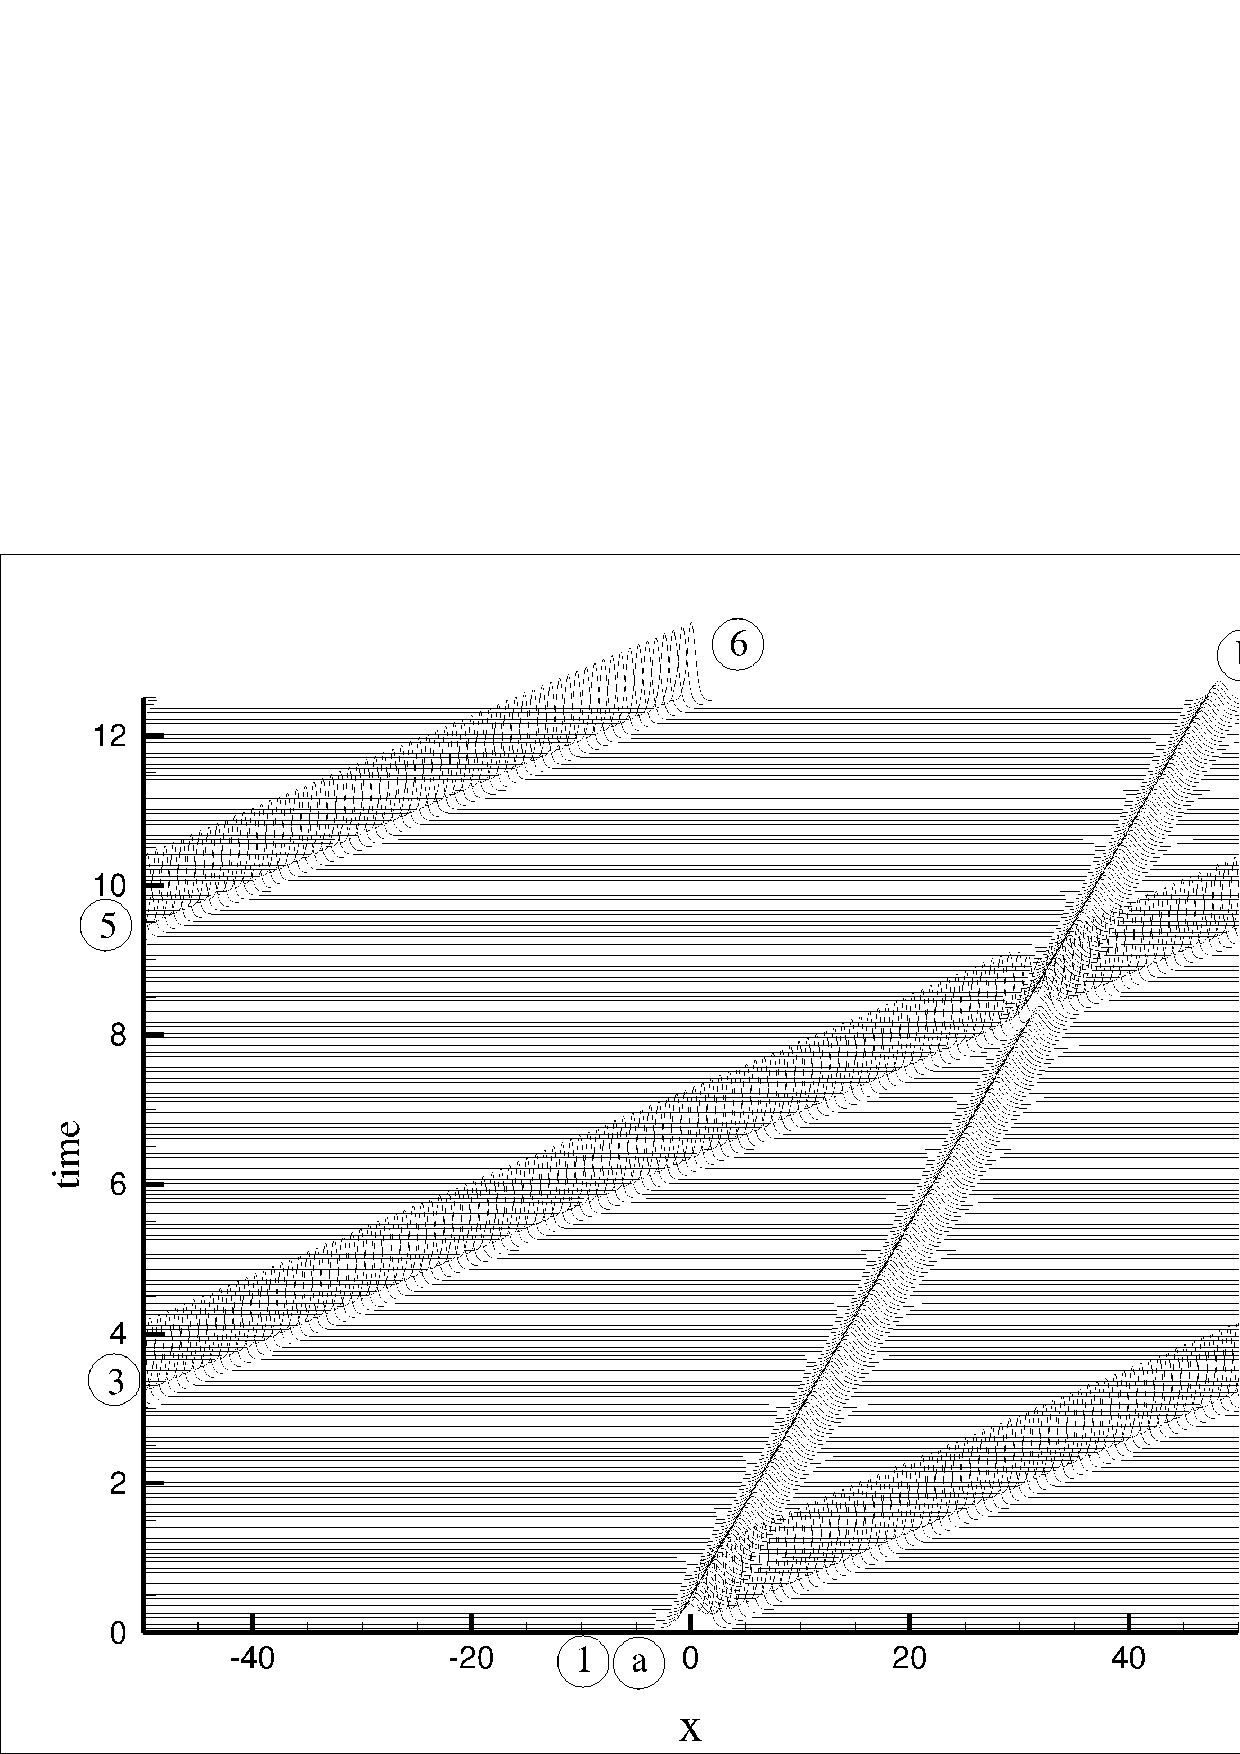
\includegraphics[width=0.65\linewidth]{Fig_14}
\caption{Nonlinear interaction of the two solitons demonstrating the phase shift.}
\label{fig:twointeract}
\end{figure}

\begin{figure}
\centerline{
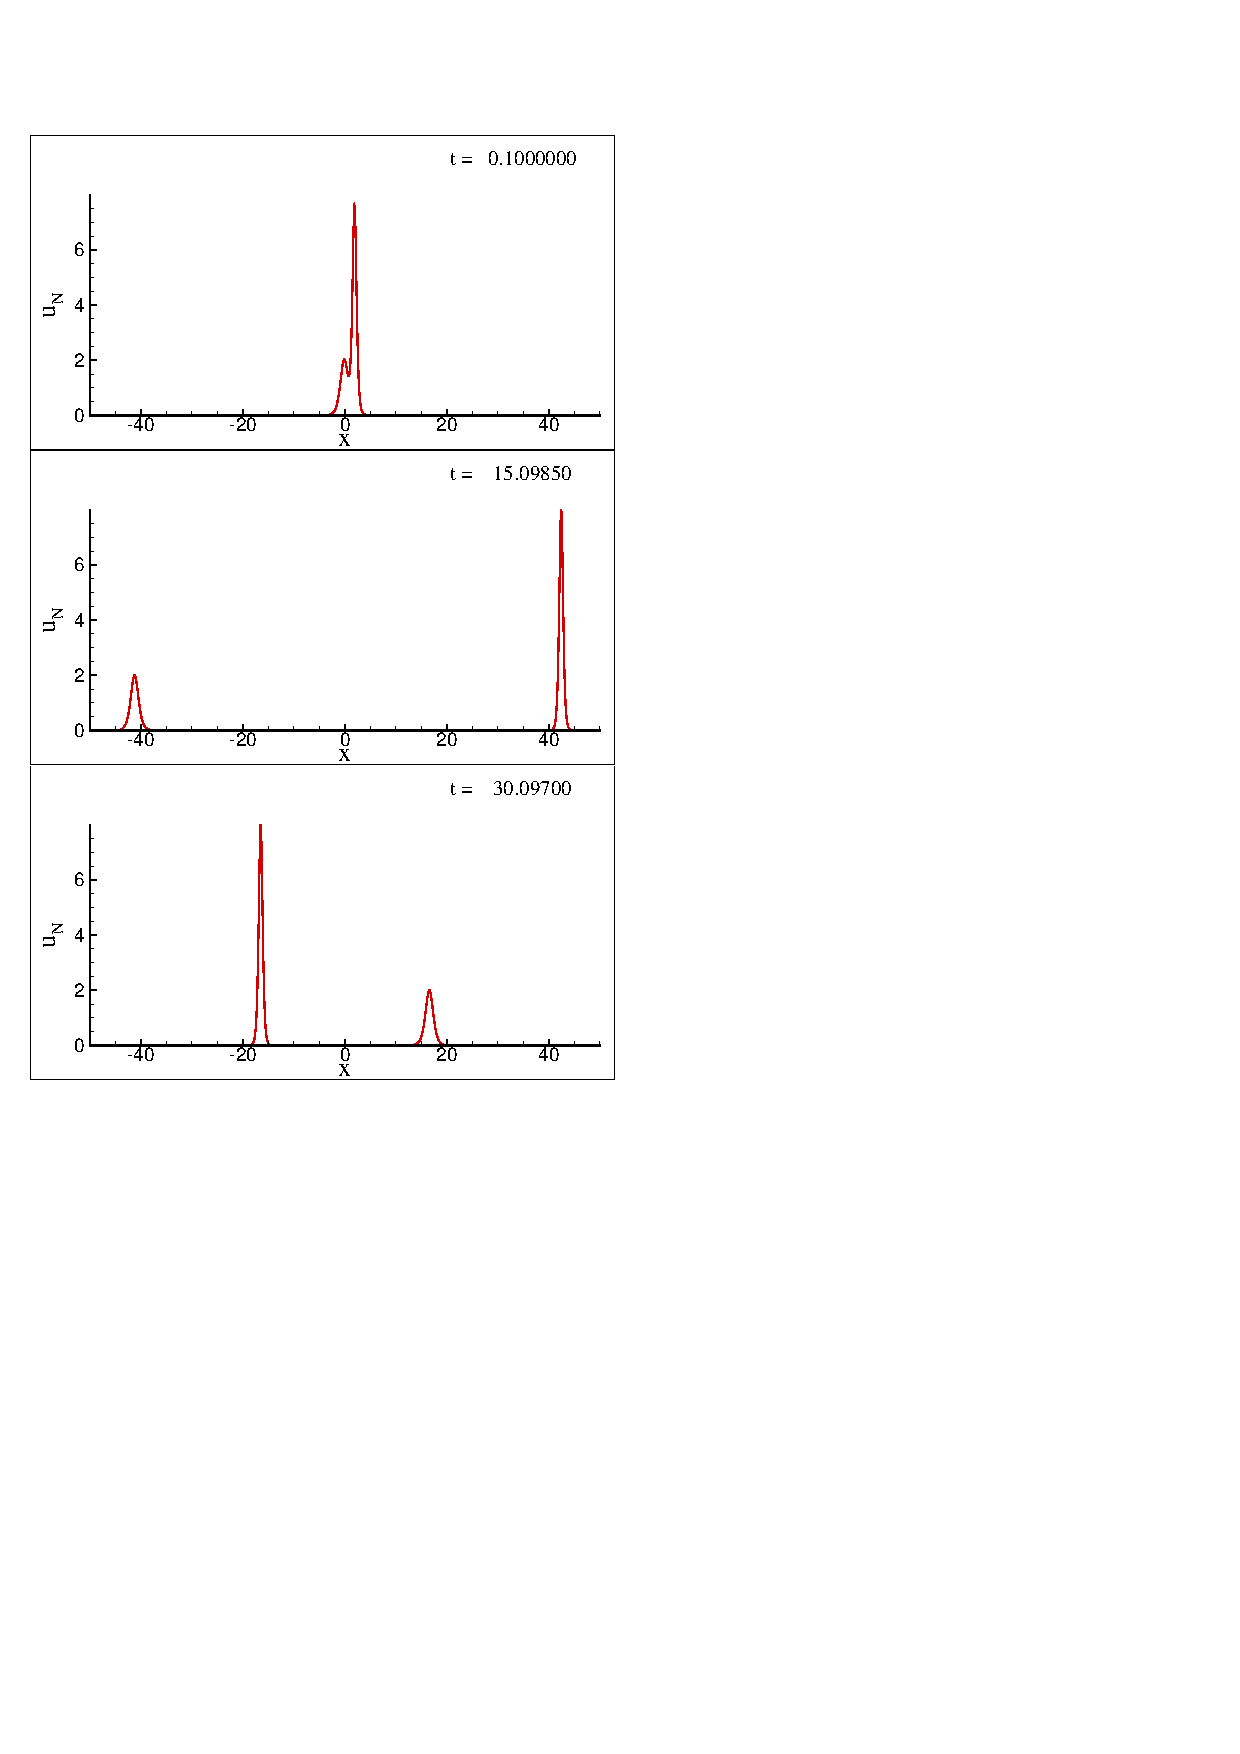
\includegraphics[width=0.5\linewidth]{Fig_15}
}
\caption{Representative numerical solution for two-soliton case, showing the location of the soliton at three time instants}
\label{fig:two1}
\end{figure}

\begin{figure}[h!]
\centerline{
\subfloat[]{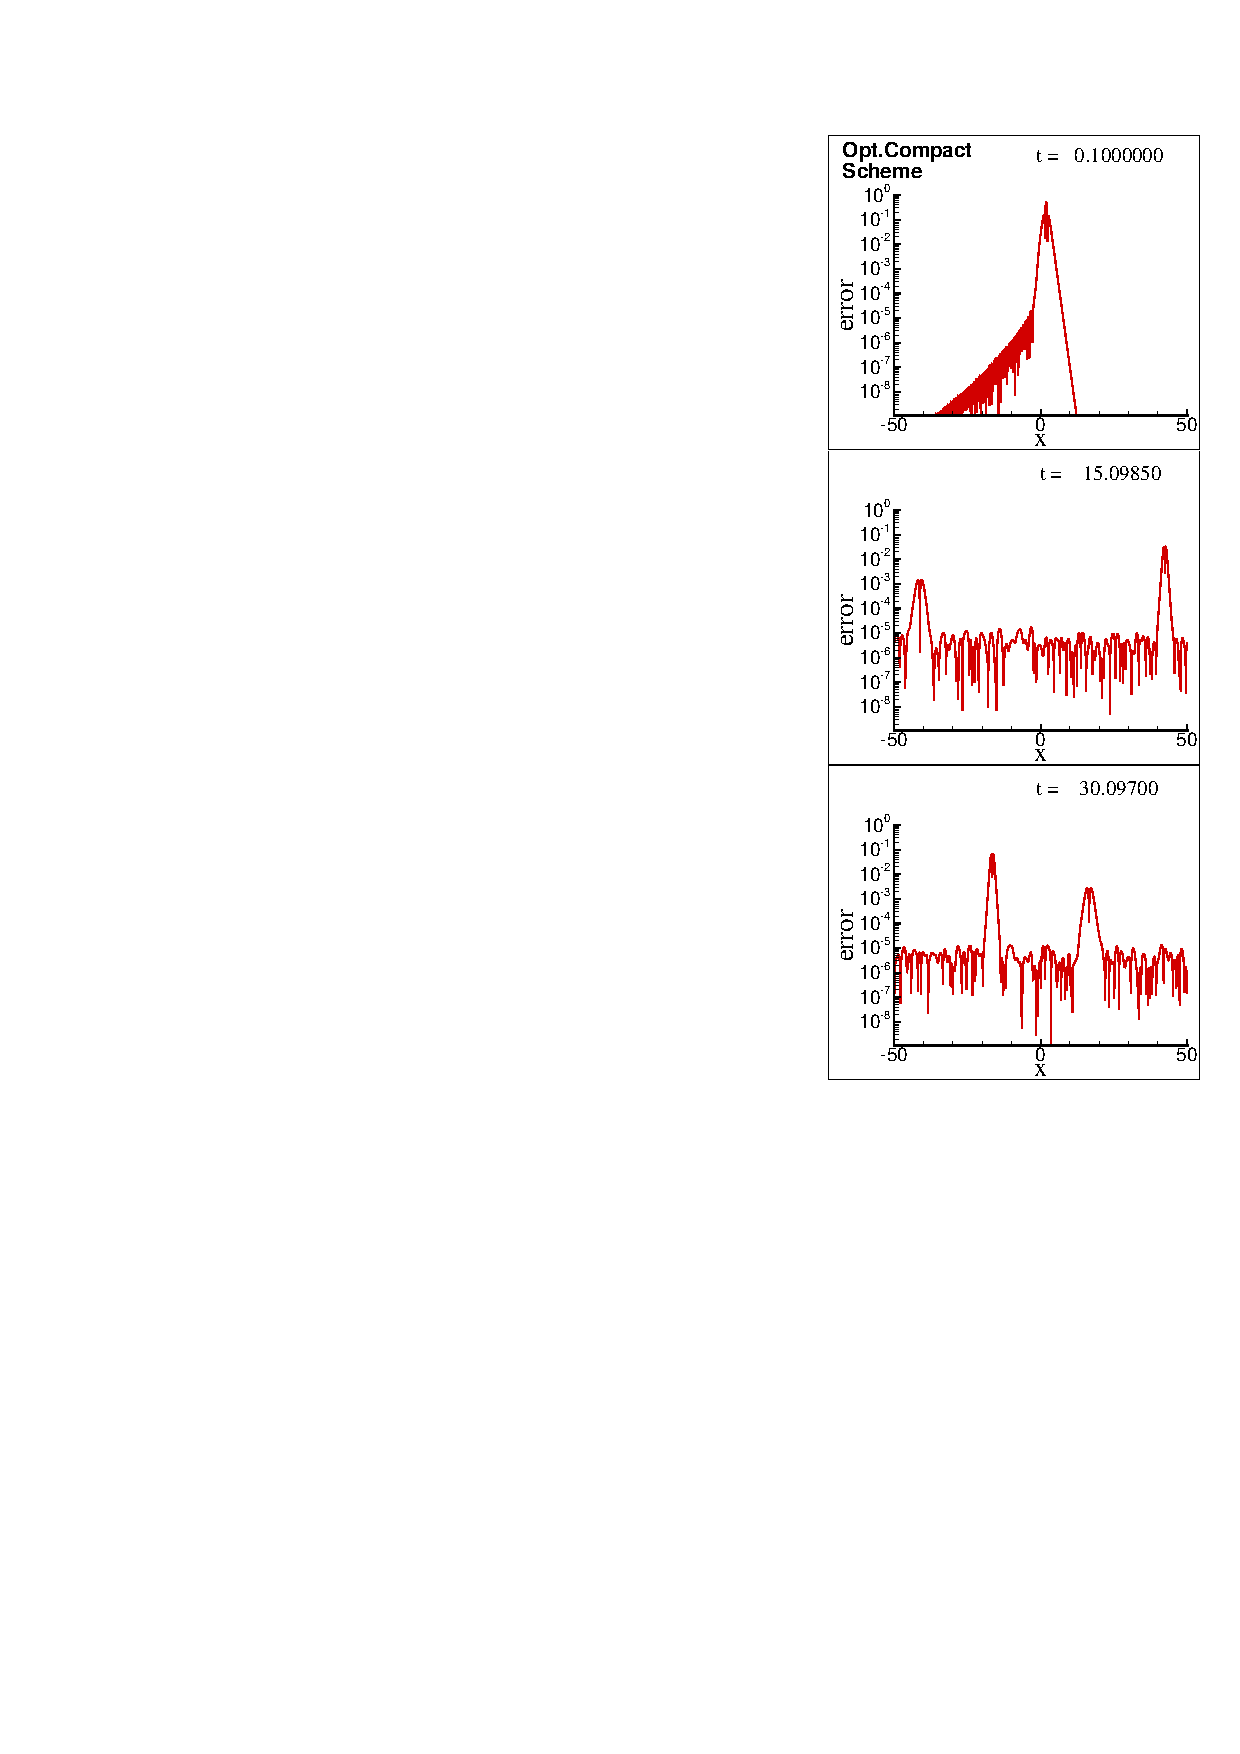
\includegraphics[width=0.33\linewidth]{Fig_16a}}
\subfloat[]{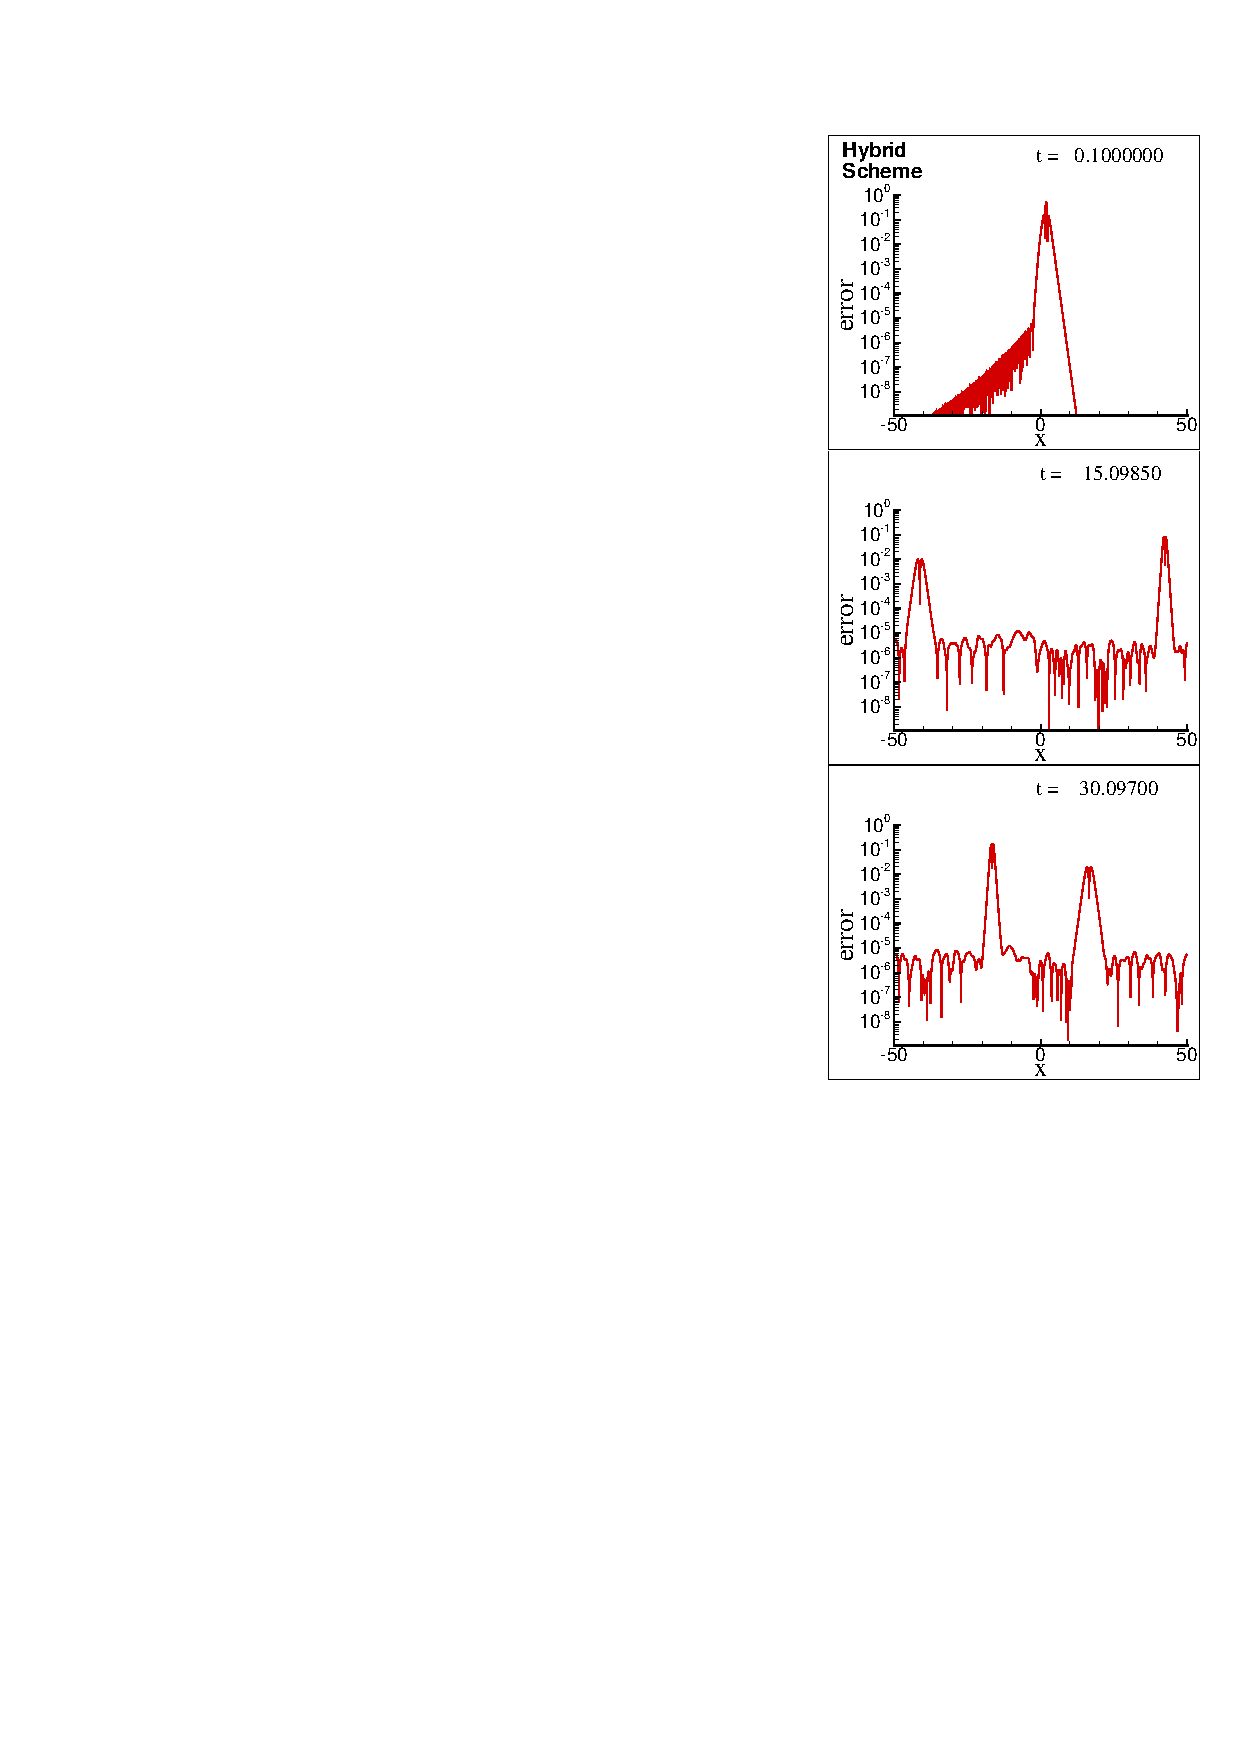
\includegraphics[width=0.33\linewidth]{Fig_16b}}
\subfloat[]{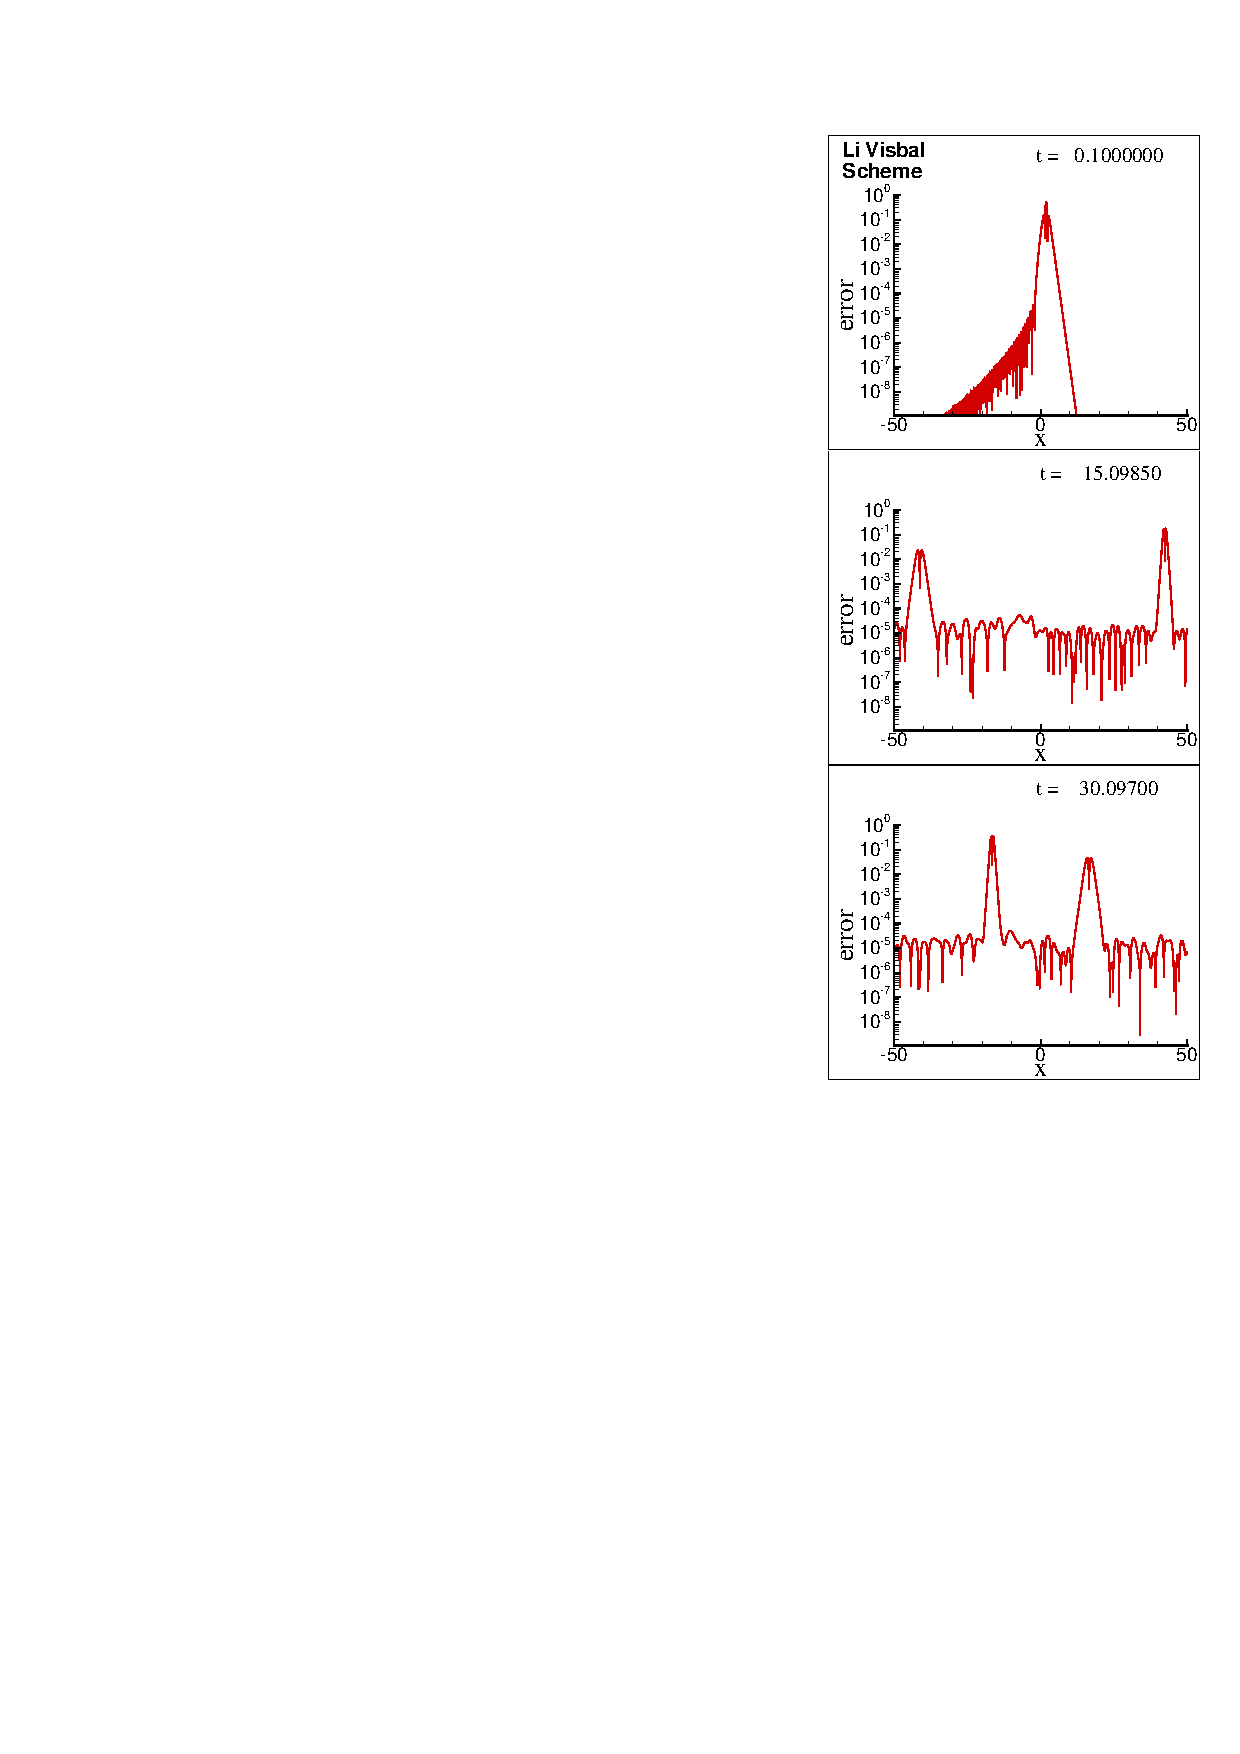
\includegraphics[width=0.33\linewidth]{Fig_16c}}
}
\caption{Evolution of error for two-soliton case comparing different methods}
\label{fig:two2}
\end{figure}
%-----------------------------------------------------------------------------------------------------

However, it is observed that a reduction in time-step from $1 \times 10^{-5}$ to $1 \times 10^{-6}$, only added to the computational cost and has hardly 
any perceptible difference in accuracy of the solution, as shown in frames (b) and (c) of Fig. \ref{fig:one1}. This is due to higher round-off error accumulation with finer time-step. In subsection \ref{subsec:ref}, we noted that the correct solution of KdV equation is maintained if the amplitude of the 
solitons are maintained as close to $A_0 = N(N+1)$ as possible, so that one can avoid Gibbs' phenomenon. Any deviation from this amplitude would trigger upstream propagating dispersive waves, as explained by $A_N = A_0 \pm \epsilon$, where $\epsilon$ is the deviation and in IST this is studied for imprecision in initial amplitude, as shown in Figs. \ref{fig:reflect} and \ref{fig:akbk}. 

We further note that due to truncation and other sources of error, the deviation from reflection potential can occur in the computed soliton in the form of transmitted and reflected waves, due to shift from the ideal values of the scattering coefficients for a reflectionless potential, $a(k)=1,b(k)=0$. 
This is investigated next for different numerical schemes studied here by simulating one-soliton case by the optimized compact scheme, the hybrid scheme and the Li-Visbal scheme with 
$N=2048$ and $\Delta t = 1 \times 10^{-5}$. The comparison of the three methods are shown in Fig. \ref{fig:one2}.
The one-soliton case is computed till $t=80$ in which it traverses the periodic domain for five cycles.  Error magnitudes vary considerably with the method chosen; especially low while using optimized compact scheme. Once again in the near-field of the soliton, absolute error shows the double peak structure, due to the presence of phase error relative to the exact solution, which has been observed to grow in amplitude with time.

For the two-soliton case, as mentioned in subsection \ref{subsec:init}, the two solitary waves in a periodic domain keep interacting as illustrated in Fig. 
\ref{fig:twointeract} computed by the hybrid scheme, with $N = 2048$ and $\Delta t =10^{-5}$. Starting from the initial location, the taller wave of amplitude eight moves along the path marked (1)-(6), which is noted in three segments due to periodicity of the domain, otherwise it is the same 
soliton with identical properties. The shorter soliton of amplitude two moves along (a)-(b) and it is moving to the right at a slower speed. 
One can clearly note the phase shift created during the nonlinear interaction of the two solitons, with the smaller amplitude soliton showing it distinctly. This establishes the correct error-free computations of the interactions, as given in the definition of multiple-solitons and their
interactions.

As in the case of one-soliton case, the error levels are investigated for the two-soliton case corresponding to three time instants as given in Fig. \ref{fig:two1}.
The evolution of error for the two-soliton case with numerical parameters of $N=2048$ and $\Delta t = 1 \times 10^{-5}$, using 
all three schemes are shown in the various frames of Fig. \ref{fig:two2}, till $t=30$. The results suggest that both the solitary waves, 
the taller and the shorter one, suffer from phase error. The amplitude of the maximum error depends on the phase shift of the solitons and is directly related to the amplitude of the soliton itself. Thus, the error variation at other locations with time is a better quantity to test the efficacy of a scheme. Again, the magnitude of error is dependent on the choice of scheme.

As the numerical solution evolves, dispersive waves due to Gibbs' phenomenon keep emerging from the left shoulder of the soliton, as indicated by the 
error in Figs. \ref{fig:one2} and \ref{fig:two2} at \emph{t=0.1}. The maximum error is in the neighborhood 
of the solitons and is very high at early times, as shown in the top frames. At other locations, initially 
the error keeps growing in amplitude and after a short time, its amplitude saturates in the domain with levels unchanged, although the spectrum changes 
due to filtering of the high wavenumber components during discretizations. Since the KdV equation is a nonlinear equation, such errors interact with the 
original soliton itself, suffering further scattering which is noted as the Gibbs' phenomenon. Smaller amplitude soliton has smaller phase error, but 
more diffused as compared to the larger soliton, which appears more localized in space. We also note that two-soliton cases suffer more error as compared to the one-soliton case.

Another interesting feature is that although the solitons move away from the initial location ($x=0$), in its immediate neighborhood there remains a distinct error structure with slightly higher magnitude in comparison to surrounding locations. This structure is stagnant, as clearly seen in the 
error plots of one-soliton case in Fig. \ref{fig:one2} at \emph{t=70} and two-soliton case in Fig. \ref{fig:two2} at \emph{t=15}. This is the trace of the initial condition left behind, 
after the solitary waves have moved from the initial location, and is also one of the sources of dispersive waves.


We have noted that the solution of KdV equation display nonlinear phenomenon and the solitons scatter error globally. The steepness of the solitons
indicate the presence of high wavenumbers in the solution. It is this presence of high wavenumbers which makes the optimized compact scheme as more 
accurate, as compared to the Li-Visbal scheme which utilizes a larger stencil. Use of larger stencil in Li-Visbal scheme also would require more boundary closure for the non-periodic cases. However, the present investigations have been performed with periodic boundary conditions and is devoid of this problem for any of the methods. The superiority of the optimized compact scheme over the other two methods is established in Fig. \ref{fig:cn_cph_comp}, displaying the $c_N/C_{ph}$ for the model dispersion equation, with $N_d =0.09$. Even for this linear equation, an area of high wavenumbers is shown hatched, where the optimized compact scheme is more accurate as compared to the other two methods. From the figure one can see that at $kh =2.62$ where the hatched region starts the $c_N/C_{ph}$ values for the optimized compact scheme, hybrid scheme and Li-Visbal scheme are $1.17011, 0.5594, 0.8430$ respectively. After $kh =2.62$ the phase error in optimized compact scheme is always smaller compared to the other two schemes. Thus, the dispersion error for nonlinear KdV equation will definitively be lower for the optimized compact scheme.  

%-----------------------------------------------------------------------------------------------------
\section{Summary and Conclusions}
\label{sec:sum}
The nonlinear KdV equation has been solved with respect to one and two soliton cases using three different numerical schemes. Unlike IST, where the errors due to imprecision in initial condition only are considered, here we have explained various sources of errors due to numerical schemes, initial condition and round-off. To compare the characteristics of the numerical schemes for third derivative, a model linear dispersive equation is considered. The correct error dynamics equation for this system is derived and different numerical properties are shown for all the three methods used.  

%-----------------------------------------------------------------------------------------------------
\begin{figure}[!h]
\center
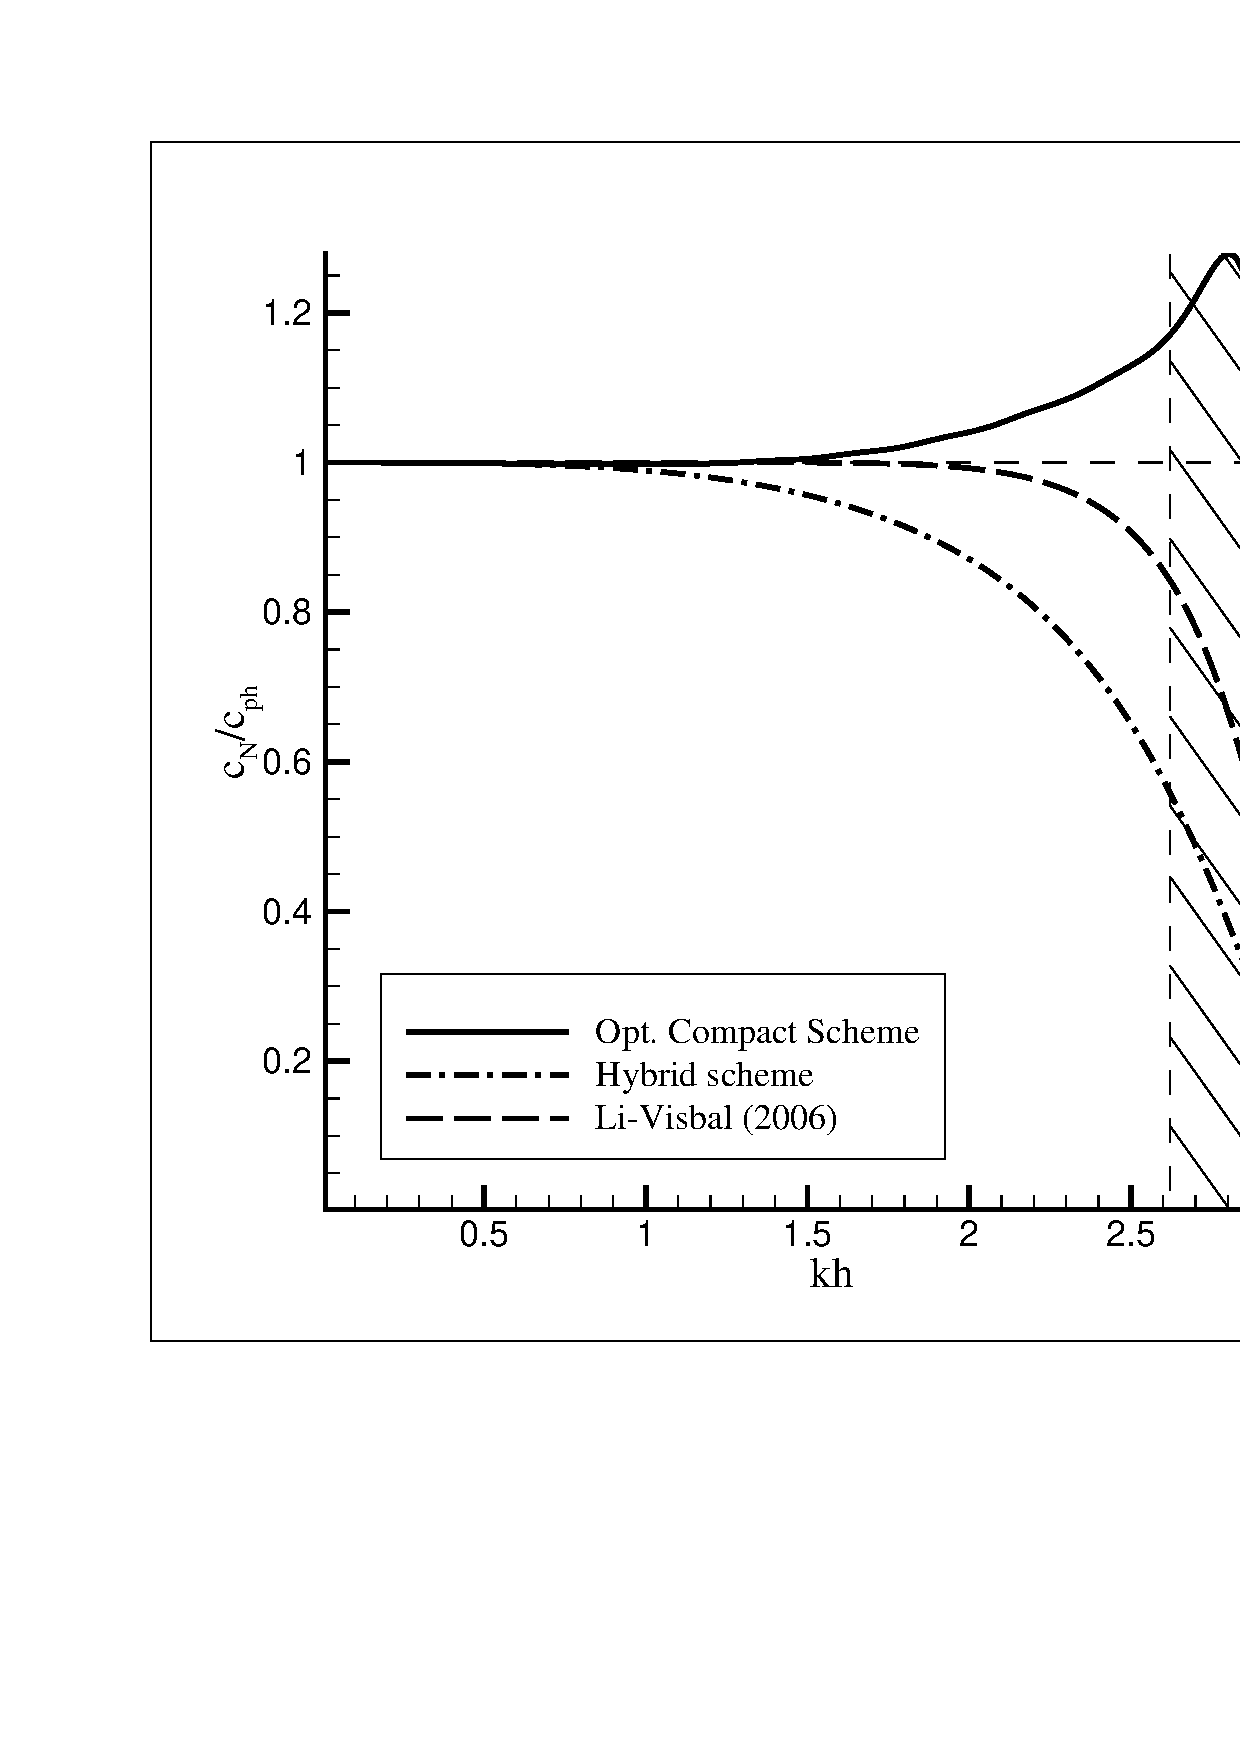
\includegraphics[width=0.5\linewidth]{Fig_17}
\caption{Comparison of $c_N/c_{ph}$ with $N_d = 0.09$ for different schemes. Hatched region indicates where the present optimized compact scheme
performs better as compared to the other two methods displayed.}
\label{fig:cn_cph_comp}
\end{figure}
%-----------------------------------------------------------------------------------------------------

The computed results of the KdV equation suggest that of the three numerical schemes compared, the optimized compact scheme offers better accuracy. The error levels of the optimized compact scheme differ by at least an order of magnitude with that of the other two. However, for the linear dispersion equation the same cannot be said.

 The hybrid CD4-OUCS3 scheme performs reasonably well, and is a remarkable improvement in terms of spectral resolution, compared to conventional explicit schemes. This scheme proves to be the fastest of the three, as it employs only one implicit compact scheme, to compute both convection and dispersion term.
 
 The Li-Visbal compact scheme shows remarkable accuracy for the simulation of one-dimensional dispersion equation, as is predicted by the error dynamics 
of the linear dispersion equation. However while simulating KdV equation, the error levels with Li-Visbal scheme are at par with the hybrid CD4-OUCS3 scheme, in spite of the scheme is of higher order.
 
  In the presence of nonlinearity, the optimized compact scheme performs better, as compared to the other two methods, in terms of accuracy. While simulation of KdV equation is a challenging problem, it can serve as a benchmark to test numerical schemes for first and third derivatives by looking 
at the response of the scheme in the presence of dominant nonlinearity.

%\section*{References}
%\newpage
\bibliographystyle{spmpsci}
%\bibliographystyle{spphys}
\bibliography{KdV-To-cite}



\end{document}
